%%%%%%%%%%%%%%%%%%%% PREAMBLE %%%%%%%%%%%%%%%%%%%%

% document
\documentclass[fleqn,usenatbib,useAMS]{mnras}

% fonts
\usepackage{newtxtext,newtxmath} % comment to switch to old Computer Modern fonts
%\usepackage{mathptmx}      % alternative Times font
%\usepackage{txfonts}       % alternative Times font
\usepackage[T1]{fontenc}    % vector fonts
\usepackage{ae,aecompl}     % vector fonts

% packages
\usepackage{graphicx}	% Including figure files
\usepackage{amsmath}	% Advanced maths commands
\usepackage{amssymb}	% Extra maths symbols
\usepackage{multicol}   % Multi-column entries in tables
\usepackage{bm}		    % Bold maths symbols, including upright Greek
\usepackage{pdflscape}	% Landscape pages
\usepackage{mathtools}  
\usepackage{silence}    
\usepackage{xspace}
\WarningFilter{latex}{Text page 1 contains only floats}

% commands
\DeclareMathOperator\arctanh{arctanh}
\DeclareMathOperator\arcsinh{arcsinh}
\DeclareMathOperator\arccosh{arccosh}
\newcommand*{\about}{\mathord\sim}
\newcommand*{\Sersic}{S\'{e}rsic\xspace}
\newcommand*{\SExtractor}{\textsc{SExtractor}\xspace}
\newcommand*{\Gnuastro}{\textsc{Gnuastro}\xspace}
\newcommand*{\NoiseChisel}{\textsc{NoiseChisel}\xspace}
\newcommand*{\Segment}{\textsc{Segment}\xspace}
\newcommand*{\MakeCatalog}{\textsc{MakeCatalog}\xspace}
\newcommand*{\PSFEx}{\textsc{PSFEx}\xspace}
\newcommand*{\GalSim}{\textsc{GalSim}\xspace}
\newcommand*{\LSSTSPs}{\textsc{LSST Science Pipelines}\xspace}
\newcommand*{\LSSTPs}{\textsc{LSST Pipelines}\xspace}
\newcommand*{\DMA}{\textsc{P6}\xspace}
\newcommand*{\DMB}{\textsc{S128}\xspace}
\newcommand*{\VRO}{Vera C. Rubin Observatory\xspace}
\newcommand*{\RO}{Rubin Observatory\xspace}
\newcommand*{\LSST}{Legacy Survey of Space and Time\xspace}

% what who where when
\title[LSB Sky Subtraction]{Sky Subtraction in an Era of Low Surface Brightness Astronomy}
\author[L.~S.~Kelvin et al.]{
\parbox{\textwidth}{
\raggedright
Lee~S.~Kelvin,$^{1,2,3}$
Imran~Hasan$^{2}$
and J.~Anthony~Tyson$^{2}$
}\vspace{0.5cm}\\
\parbox{\textwidth}{
$^{1}$Department of Astrophysical Sciences, Princeton University, 4 Ivy Lane, Princeton, NJ 08544, USA\\
$^{2}$Department of Physics, University of California, One Shields Ave., Davis, CA 95616, USA\\
$^{3}$Astrophysics Research Institute, Liverpool John Moores University, IC2, LSP, 146 Brownlow Hill, Liverpool, L3 5RF, UK\\
}
\vspace{-0.75cm}
}
\date{Accepted XXX. Received YYY; in original form ZZZ}
\pubyear{2021}

% finish up preamble
\begin{document}
\label{firstpage}
\pagerange{\pageref{firstpage}--\pageref{lastpage}}
\maketitle

%%%%%%%%%%%%%%%%%%%%%%%%%%%%%%%%%%%%%%%%%%%%%%%%%%

%%%%%%%%%%%%%%%%%%%% ABSTRACT %%%%%%%%%%%%%%%%%%%%

\begin{abstract}
The \VRO wide-deep LSST sky survey will reach unprecedented surface brightness depth over tens of thousands of square degrees. Surface brightness photometry has traditionally been a challenge. Current algorithms which combine object detection with sky estimation systematically over-subtract the sky, biasing surface brightness measurements at the faint end and destroying or severely compromising low surface brightness light. While it has recently been shown that properly accounting for undetected faint galaxies and wings of brighter objects can in principle recover a more accurate sky estimate, this has not yet been demonstrated in practice. Obtaining a consistent spatially smooth underlying sky estimate is particularly challenging in the presence of representative distributions of bright and faint objects. In this paper we report on realistic forward \GalSim simulations based on deep Subaru HSC data which have the twin advantages of a natural object distribution and known underlying simulated sky. Simulations of both crowded and uncrowded fields are run, as well as tests for dependence on galaxy type and limiting flux for detection. We test several photometry packages on these simulated data, in addition to several configuration modes, and compare their performance at extreme low surface brightness. We find that the \Gnuastro software package outperforms other detection packages in most cases, typically recovering an estimated sky value which is closest to the injected sky background. We additionally find that the application of the modelled masking procedure presented in this paper to the \SExtractor source detection package has several unique advantages, producing extremely faint output sky estimates, providing high fidelity output science catalogues, and performing optimally in deep crowded fields.
\end{abstract}

\begin{keywords}
techniques: image processing -- methods: observational -- surveys -- galaxies: structure -- galaxies: general -- galaxies: fundamental parameters
\end{keywords}

%%%%%%%%%%%%%%%%%%%%%%%%%%%%%%%%%%%%%%%%%%%%%%%%%%

%%%%%%%%%%%%%%%%% BODY OF PAPER %%%%%%%%%%%%%%%%%%

\section{Introduction}
\label{sec:introduction}

The human eye and brain is unique in its capacity to look up at the night sky and easily separate a wide variety of astronomical objects from the all encompassing celestial sphere upon which they lay. A computer, however, finds such a task decidedly non-trivial, often requiring extensive training, testing, and the use of a bespoke data processing pipeline. Tasks such as object detection, segmentation, point source estimation, and, crucially, sky estimation are all important components of many professional image processing pipelines. Deriving algorithms to accurately and rapidly perform such tasks has been an active area of research over the last several decades, with the issue becoming more pressing in recent years as we rapidly enter an era of big data astronomy which combines wide surveyed areas with unprecedented depth. 

Contemporary astronomical observatories are located at sites with optimal seeing, photometric stability, and dark skies. Extremely dark ground-based sites with little to no light pollution are able to achieve sky brightness levels down to $\mu_V\sim22\;\mathrm{mag\;arcsec}^{-2}$ \citep{Garstang1989}. Without the impediment of an atmosphere, space-based facilities such as the Hubble Space Telescope (HST) are able to probe $\sim1-2\;\mathrm{mag\;arcsec}^{-2}$ deeper still \citep[see, e.g.,][and references therein]{Knapen2017}. Taking full advantage of such sites in combination with a careful observing strategy and a minimally aggressive sky subtraction technique now allows us to probe beyond the $\mu=30\;\mathrm{mag\;arcsec}^{-2}$ threshold on an increasingly regular basis \citep{Iodice2016,Trujillo2016}. Such methodologies allow for formerly hidden galaxy structures to be seen and catalogued for the first time \citep[e.g.,][]{Kelvin2018}. The previously hidden Universe in the low surface brightness (LSB) regime continues to unveil a wealth of information across multiple scales, from LSB-type dwarfs \citep{vanDokkum2015,Williams2016} to circumgalactic stellar haloes \citep{D'Souza2014,Wang2019} and the mass-merging remnant intracluster light \citep{Montes2014,Montes2018,Montes2019}. 

Optimal observing conditions notwithstanding, features of the background sky must still be characterised and removed prior to scientific analyses. A typical sky component consists of scattered light from astronomical sources (e.g., stars, cirrus, airglow) and scattered light from optics within the telescope \citep{Karabal2017}. Additional contaminant flux such as satellite trails \citep{Cheselka1999,Vandame2001,Storkey2004}, cosmic rays \citep{Fixsen2000}, CCD edge effects \citep{Goldstein2015} and saturation features \citep{Desai2016} all impact any estimation of the sky, and typically must also be accounted for and removed as part of the background estimation process. 

The process begins with automated photometry and the detection of individual objects. This is a multi-step process which becomes more challenging at faint surface brightnesses. One of the first such software packages to address this task across a wide dynamic range and for faint galaxies was the Faint Object Classification and Analysis System (\textsc{FOCAS})~\cite{Jarvis1981}. Using non-parametric statistical pattern recognition, it was initially driven by the need for surface photometry on faint co-added photographic plates, and later was extensively used on even fainter CCD data. The output of a Bayesian detection algorithm with optimal filter and adjustable detection threshold is fed to an area assembly stage, followed by spatial segmentation, iterative sky level estimation, object photometry, a hypersurface classifier, and output catalogue containing the segmentation history of each object. Recursive \textsc{FOCAS} runs on deep CCD data asymptotically reach completeness at the noise level. The program has many adjustable parameters: detection threshold, sky histogram, detection filter, segmentation sensitivity, intensity moments weighting kernel, and objects classification parameters. 

A subsequent streamlined software package based upon similar operating principles, \SExtractor \citep{Bertin1996}, was developed for faster automated photometry. While based partly on similar precepts to that of \textsc{FOCAS}, it was designed to have a more global and computationally efficient segmentation algorithm, necessarily trading some control over optimal filters in each phase that was present in \textsc{FOCAS}. The \SExtractor package however is capable of covering a wider range of object sizes and also outputs a sky estimation map and a detected source catalogue. For sky estimation, the local background around objects is clipped iteratively at $\pm3\sigma$ around the sky median. Like a single-pass FOCAS, it produces a sky that is biased high. The \SExtractor software package has been instrumental in the development of several image processing pipelines in recent years, notably the \textsc{Galaxy Analysis over Large Areas: Parameter Assessment by GALFITting Objects from SEXTRACTOR} \citep[\textsc{GALAPAGOS};][]{Barden2012,Hiemer2014} package and the \textsc{Structural Investigation of Galaxies via Model Analysis} \citep[\textsc{SIGMA};][]{Kelvin2010,Kelvin2012} package, both of which have been used to rapidly process and analyse millions of galaxies across multiple wavelengths using data from a wide variety of surveys.

More recently, the \textsc{Gnu Astronomy Utilities} \citep[\Gnuastro;][]{Akhlaghi2015} software package has been released, providing a suite of programs and functions for use in the manipulation of astronomical data. One such constituent program is \NoiseChisel, a program for the detection of faint, extended, nebulous astrophysical objects. \NoiseChisel relies on a non-parametric algorithm rather than any particular function or fitting technique to identify contiguous regions whose noise properties are altered by the underlying faint astrophysical objects buried beneath. Other signal processing algorithms, like those mentioned above, are biased towards detecting objects that are sufficiently similar to the detection kernel being used. As \NoiseChisel does not depend on knowing the shapes or profiles of sources beforehand, and does not require any a priori knowledge of the spatial properties of astrophysical objects, it is therefore unbiased in this regard. Counter to the top-down operating principles of many prior source detection software packages, \NoiseChisel operates on a bottom-up philosophy, attempting first to characterise the background noise in an image before classifying the residual signal flux. This approach has potential advantages in the detection and characterisation of LSB light, as further discussed later in this study. 

A modern detection algorithm is being developed for use with the \VRO (hereafter, \RO), formerly known as the Large Synoptic Survey Telescope, which will undertake a 10-year deep-wide-fast survey of the southern sky called the \LSST \citep[LSST,][]{Ivezic2019}. A version of this software is currently used in the data reduction pipeline for the Hyper Suprime Cam Subaru Strategic Program \citep[HSC-SSP;][]{Aihara2018a,Aihara2018b,Bosch2018,Bosch2019}. This algorithm first identifies high signal-to-noise stars on the stellar locus, using these to model the spatially varying PSF over the entire image and subsequently facilitating characterisation of simply connected regions above a given detection threshold as detections (see Section \ref{sec:dmstack2018} for further details). Detected sources are then masked, so a polynomial model can be fit to the remaining pixels to evaluate a sky background model. This process is repeated iteratively at the CCD level until a final PSF model, detection catalogue, and sky background model are achieved. 

Many contemporary astronomy image reduction pipelines do not accurately preserve LSB flux, destroying this information at the sky subtraction phase. Furthermore, information on the undetected extragalactic background light (EBL), primarily due to fainter galaxies, is often not taken into account. These programs operate top-down: first detecting objects above a running biased initial sky estimate, then iteratively estimating object and sky fluxes. This tends to produce good photometry at higher surface brightness, but is subject to sky bias due to undetected very faint galaxies. As discussed above, a complementary approach is to work bottom-up: first estimating sky, building a sky model, and only then detecting and measuring individual objects in a final step. The key towards facilitating science at ultra low surface brightnesses is in producing accurate and robust sky estimations. 

When reducing and analysing astronomical imaging data, it is often best to separate the two tasks of sky estimation and catalogue generation (e.g., object photometry). A Bayesian statistical approach to sky estimation which uses the known faint galaxy counts has recently been pursued by \cite{Ji2018}. It was shown in simulations that robust sky precision of $\about4\,\mathrm{ppm}$ is in principle possible. In this study, we explore a number of alternative background estimator configurations which are shown to be more accurate and less affected by the extended surface brightness profiles of galaxies and the density of the local image environment as compared to traditional techniques. One challenge to be addressed is the performance over realistic large deep fields with a broad range of object densities and sizes, in addition to navigating the potentially treacherous additional components of sky background such as dust. Building upon prior efforts in this field, we present a range of sky estimation configurations which are designed to accurately preserve sky flux over large fields in realistic deep imaging, paving the way for future LSB science cases. For a fully realistic approach, we apply these configurations to full image simulations based upon recent deep survey imaging, testing the robustness of sky estimation outputs and source photometry for each.

The remainder of this paper is structured as follows. Section \ref{sec:hsc} presents our input observed dataset, imaging taken from the Hyper Suprime-Cam Subaru Strategic Program, and details the generation of our input data sample. Section \ref{sec:galsim} fully describes the generation of our simulated dataset using the \GalSim software package. Section \ref{sec:sextraction} discusses all sky estimation software packages and distinct software configurations explored within this study. Finally, our results and discussion are presented in Section \ref{sec:results}, and our conclusions are summarised in Section \ref{sec:conclusions}. For file storage purposes, FITS imaging has been compressed/uncompressed using both the NASA HEASARC \textsc{fpack}/\textsc{funpack} compression format \citep{Pence2009,Pence2010} and the GNU Gzip\footnote{\url{https://www.gnu.org/software/gzip}} compression format\footnote{With the former preferred for noisy float-type imaging and the latter for integer-type or truncated floating point data.}. All data and associated code produced for use within this study has been archived on the \textsc{GitHub} hosting platform\footnote{\url{https://github.com/leeskelvin/sci2020-lsbskysub}}.

\newpage

\section{The Hyper Suprime-Cam Subaru Strategic Program}
\label{sec:hsc}

To ascertain the veracity of any given sky subtraction methodology, a real-world observed dataset is required upon which to base a subsequent series of complex simulations. To fill this role, we opt for data taken from the Hyper Suprime-Cam \citep[HSC,][]{Miyazaki2012,Miyazaki2018} Subaru Strategic Program \citep[SSP,][]{Aihara2018a}. The HSC is an $870$ megapixel prime focus camera consisting of $116$ 2k $\times$ 4k $0.168\;\mathrm{arcsec}/\mathrm{pixel}$ CCDs mounted on the $8.2\mathrm{m}$ Subaru telescope at Mauna Kea in Hawaii. HSC-SSP survey data is segregated into three distinct layers: Wide ($1400\;\deg^2$), Deep ($27\;\deg^2$) and UltraDeep ($3.5\;\deg^2$), the former of which is utilised here. Wide-layer optical imaging is provided in the $g$, $r$, $i$, $z$ and $y$ broad-band filters, with a typical $5\sigma$ point source depth of $r\about26\;\mathrm{mag}$. Unless otherwise stated, primary analyses throughout the remainder of this study are based upon HSC-SSP $r$-band data. 

The HSC-SSP Public Data Release 1 \citep[PDR1\footnote{\url{https://hsc-release.mtk.nao.ac.jp}},][]{Aihara2018b} dataset used in this study spans $\about100\;\deg^2$ from the initial 12 month observing period, providing full-depth, reduced, calibrated imaging and relevant associated catalogue data. PDR1 full-depth co-added imaging is stored in a hierarchical format. Top level $2.82\;\deg^2$ `tracts' are organised to efficiently tile across the entire survey region, with each tract further subdivided into $9\times9$ slightly overlapping `patches' of $0.038\;\deg^2$. HSC-SSP PDR1 imaging data is processed using the \textsc{hscPipe~4} pipeline \citep{Bosch2018,Huang2018}; an HSC-specific customisation of the \RO \citep[formerly Large Synoptic Survey Telescope,][]{Ivezic2008} Data Management (DM) software stack \citep{Juric2017}, which itself is based upon concepts initially developed for use within the Sloan Digital Sky Survey (SDSS) Photo pipeline \citep{Lupton2001}. The \textsc{hscPipe~4} pipeline is tasked with a number of processing steps, summarised briefly here: initial raw data acquisition; single-visit CCD image calibration (e.g., bad pixel mask, bias correction, flat-fielding); sky estimation; PSF generation; source extraction, segmentation and deblending; pixel resampling; and image co-addition. Full details of this processing pipeline, notably the sky estimation methodology, can be found in \citet{Bosch2018} and references therein. The significant depth, multi-wavelength aspect, wide area coverage, and data-processing synergies with prior and future imaging surveys make the HSC-SSP an ideal candidate for further exploration of contemporary sky-subtraction algorithms. We note that a subsequent data release has occurred since the primary analyses within this paper were conducted. A summary of the updates provided within this data release, and their potential impact on our analyses, is discussed in Section \ref{sec:results}. 

\subsection{High/Low Density Sample Regions}
\label{sec:sample}

It is fair to assume that sky estimation routines perform differently in regions of differing source density. To that end, we require two sample regions upon which to base our subsequent simulations: one of relatively low source density and one of relatively high source density. A pseudo-random list of $57$ unique tract-patch pairs\footnote{All $57$ tract-patch pairs: 8279-07, 8280-18, 8281-28, 8282-37, 8283-38, 8284-47, 8285-27, 8520-03, 8521-46, 8522-50, 8523-51, 8524-52, 8525-53, 8526-21, 8762-00, 8763-14, 8764-15, 8765-22, 8766-23, 8767-24, 8768-61, 9314-08, 9315-48, 9316-57, 9317-58, 9318-17, 9346-16, 9347-41, 9348-42, 9349-26, 9370-02, 9371-36, 9372-43, 9373-44, 9374-45, 9375-31, 9557-06, 9558-55, 9559-56, 9560-62, 9561-40, 9562-54, 9589-05, 9590-32, 9591-33, 9592-20, 9613-01, 9614-30, 9615-34, 9616-35, 9617-25, 9618-60, 9800-04, 9801-11, 9802-12, 9803-13, 9804-10.} is generated from the HSC-SSP PDR1 dataset, providing an unbiased sample of HSC imaging data across a wide area. The $r$-band coadded calibrated exposure (\texttt{deepCoadd\_calexp}) data products containing the \textsc{hscPipe~4} background-subtracted science images, pixel masks and variance maps are downloaded for each of these tract-patch pairs. 

In order to provide an initial estimate of field density for each tract-patch region, the \SExtractor \citep{Bertin1996} source detection software package (version 2.19.5) is applied to each science image. \SExtractor is operated using mostly the default configuration setup\footnote{Default \SExtractor configuration file and parameter list generated on the command line using \texttt{sextractor -dd} and \texttt{sextractor -dp}, respectively. Default \SExtractor neural network and convolution file taken from \url{https://astromatic.net/redmine/projects/sextractor/repository/revisions/332/show}.}, with the exception of detection threshold which is fixed to an absolute value of $0.07$ counts. The default operation of \SExtractor defines sources as those with significant flux above a $1.5\sigma$ background threshold. Maintaining such a relative threshold across each tract-patch pair would introduce a sky estimation dependency on source density, and unfairly bias against regions where the initial estimation of the background is inaccurate. Preliminary testing of our dataset found that an absolute threshold of $0.07$ counts is sufficient to provide an unbiased estimate of source density for each tract-patch pair in these data. See Section \ref{sec:thresholds} for more information on the derivation of this absolute detection threshold level. Using this absolute detection threshold, \SExtractor is once again ran on all $57$ tract-patch regions, generating an estimate of field density in addition to a host of per-object parameters particular to each detected object\footnote{Our output \SExtractor catalogue parameters are: \texttt{NUMBER}, \texttt{FLUX\_AUTO}, \texttt{MAG\_AUTO}, \texttt{KRON\_RADIUS}, \texttt{PETRO\_RADIUS}, \texttt{BACKGROUND}, \texttt{THRESHOLD}, \texttt{X\_IMAGE}, \texttt{Y\_IMAGE}, \texttt{A\_IMAGE}, \texttt{B\_IMAGE}, \texttt{THETA\_IMAGE}, \texttt{ELLIPTICITY}, \texttt{CLASS\_STAR} and \texttt{FLUX\_RADIUS}. A full description of each parameter may be found in \citet{Bertin1996}}.

Recovered field densities for all tract-patch regions are shown in Figure \ref{fig:patchden}. Values range from $\about40$ to $\about100$ objects per square arcminute ($\about150000$ to $\about350000$ objects per square degree). To select two sample fields, we exclude outliers at both the extreme low density and high density terminus of this range, and select the tract-patch regions located at the 5th and 95th percentiles of recovered field density. The fields found at these percentiles are used as the bases for our low and high density regions, respectively. Tract-patch 8283-38 represents our low density region, containing $6813$ detected objects ($\about45\,\mathrm{N_{obj}\,/\,arcsec^2}$ or $\about181991\,\mathrm{N_{obj}\,/\,sq.\,deg}$), whilst tract-patch 9592-20 represents our high density region, containing $12183$ detected objects ($\about90\,\mathrm{N_{obj}\,/\,arcsec^2}$ or $\about325435\,\mathrm{N_{obj}\,/\,sq.\,deg}$). 

\begin{figure}
    \centering
    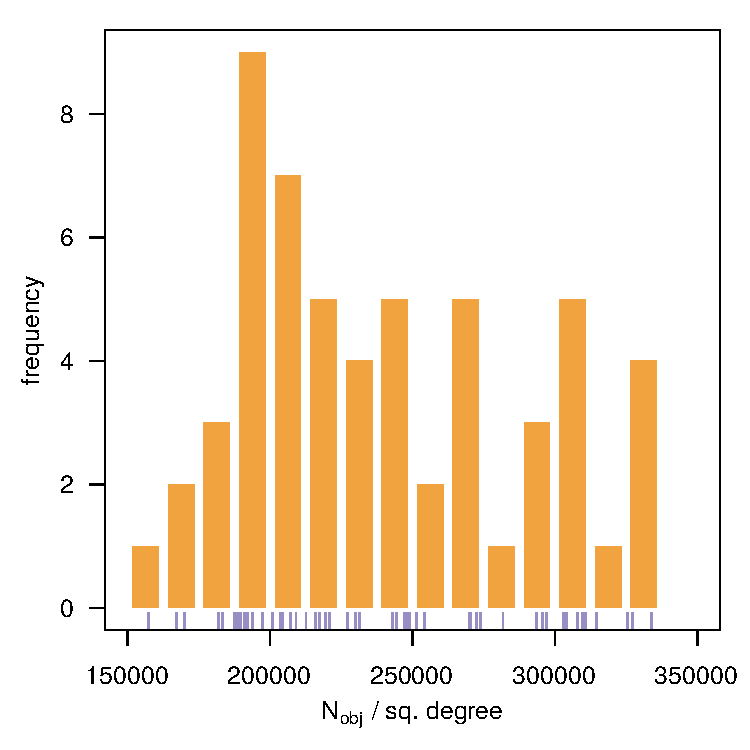
\includegraphics[width=\columnwidth]{{{fig/patchden}}}
    \caption{Initial estimate of field density for all $57$ tract-patch regions using a constant absolute detection threshold of $0.07$ counts. Each patch is approximately $0.196\;\deg$ on a side. Using these data, we select the tract-patch fields located at the 5th and 95th percentiles of recovered field density to respectively represent our low-density and high-density input observed datasets.}
    \label{fig:patchden}
\end{figure}

Postage stamps and associated segmentation maps for the low density (tract-patch 8283-38) and high density (tract-patch 9592-20) regions can be found in Figures \ref{fig:stamplo} and \ref{fig:stamphi}, respectively. These figures are arranged, clockwise from top left, thus: RGB postage stamp of the entire $706\times689\;\mathrm{arcsec}$ region; $r$-band postage stamp; $r$-band segmentation map; and RGB postage stamp for a $90\times88\;\mathrm{arcsec}$ zoomed cutout. All postage stamps are arctan scaled and smoothed with a Gaussian kernel of $\Gamma=3\;\mathrm{pix}$. RGB images are generated using HSC-SSP PDR1 $z$, $i$ and $r$ passbands. Shades of grey within the segmentation map are randomly assigned to aid in the visual separability of neighbouring objects. As can be seen, the relatively high resolution and depth of the HSC dataset make these data an ideal candidate for further exploration of sky-subtraction methodologies. Several imaging artefacts remain in these data, notably, central saturation and diffraction spikes associated with bright point sources, optical ghosts, and shredding of bright objects. Whilst these artefacts do not severely impact our subsequent analyses, we highlight them here for reference. 

\begin{figure*}
\begin{tabular}{rl}
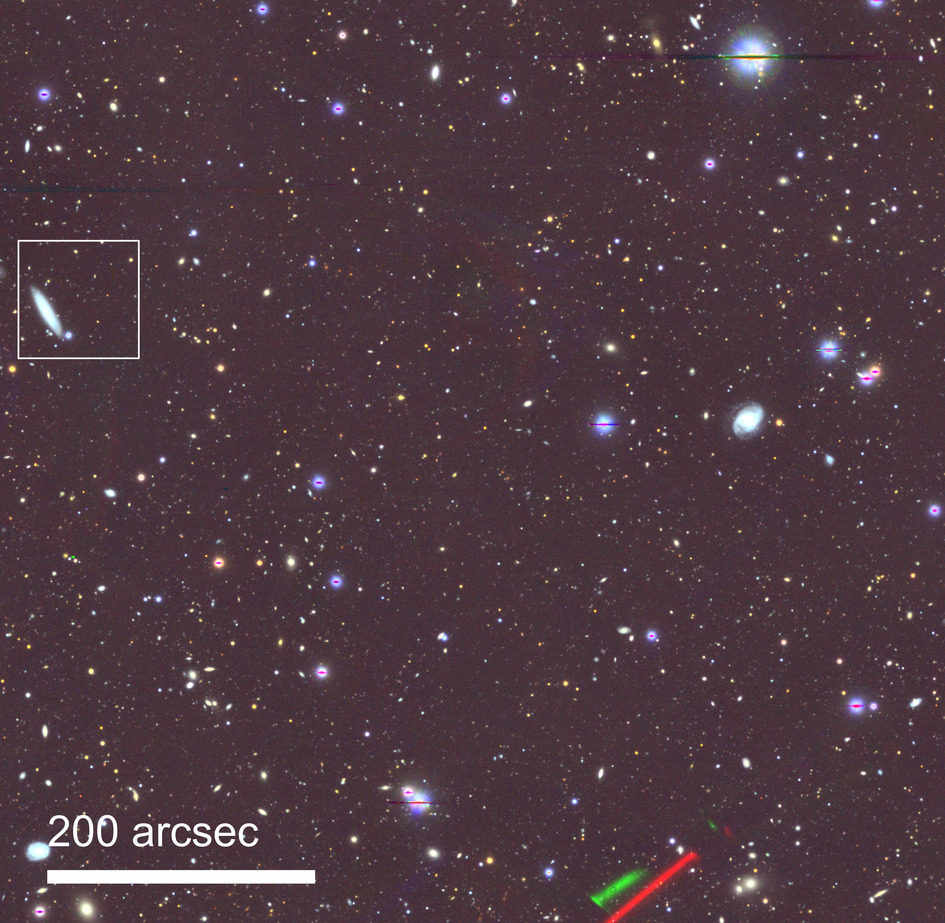
\includegraphics[width=\columnwidth]{{{fig/calexp-HSC-ZIR-8283-38.fullrgb}}}
&
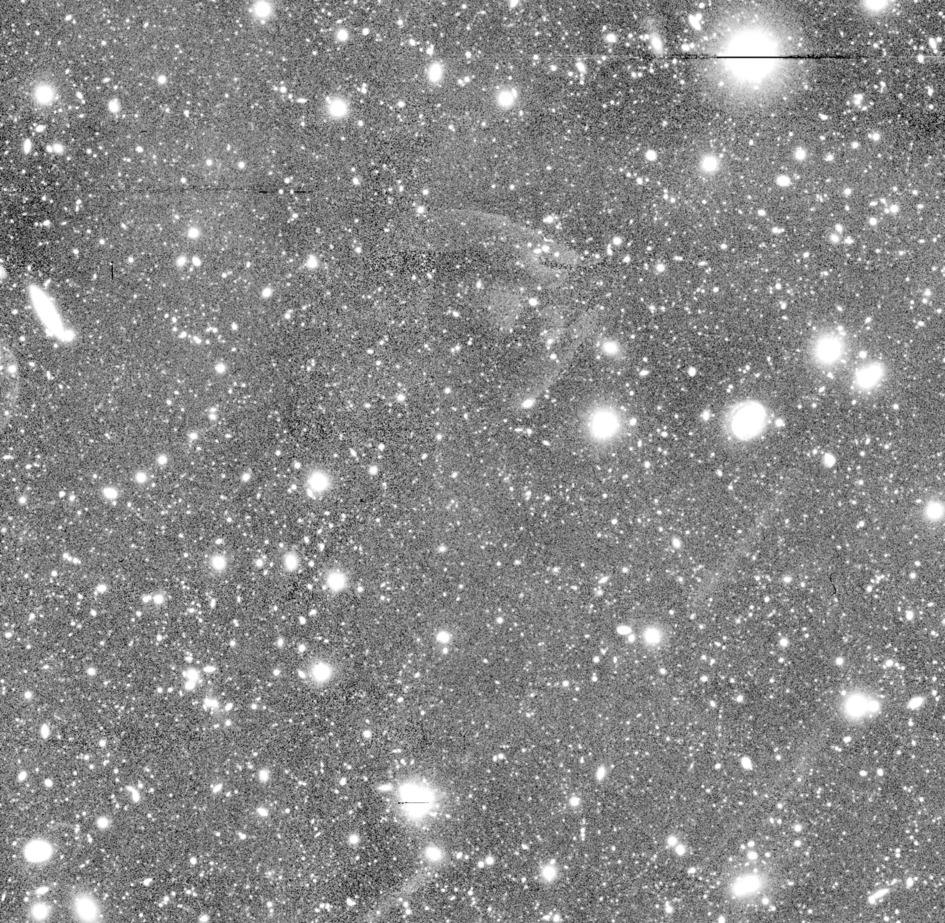
\includegraphics[width=\columnwidth]{{{fig/calexp-HSC-R-8283-38.fullmon}}}
\\\\
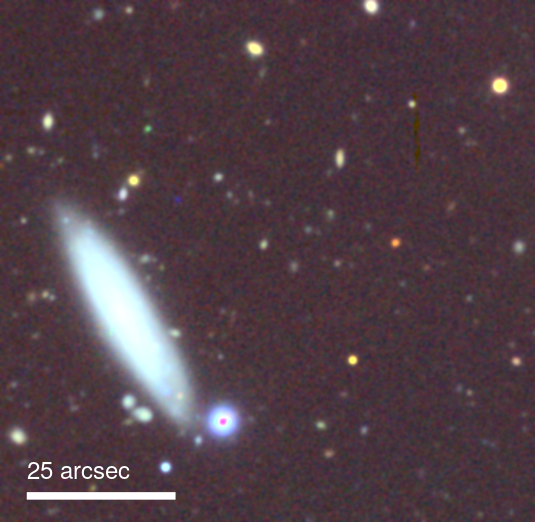
\includegraphics[width=\columnwidth]{{{fig/calexp-HSC-ZIR-8283-38.zoomrgb}}}
&
\frame{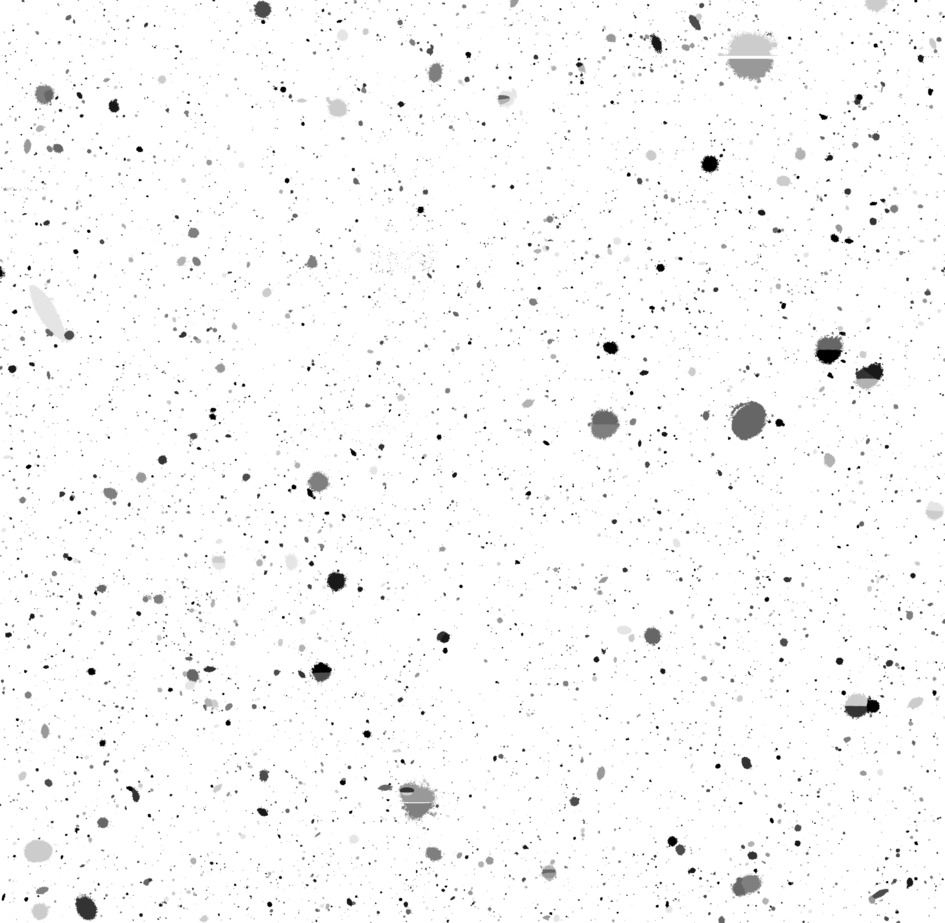
\includegraphics[width=\columnwidth]{{{fig/calexp-HSC-R-8283-38.segmap}}}}
\end{tabular}
\caption{HSC-SSP PDR1 low density region, tract-patch 8283-38. Clockwise from top left: RGB postage stamp of the entire $706\times689\;\mathrm{arcsec}$ region; $r$-band postage stamp; segmentation map; and RGB postage stamp for a $90\times88\;\mathrm{arcsec}$ zoomed cutout. All postage stamps are arctan scaled and smoothed with a Gaussian kernel of $\Gamma=3\;\mathrm{pix}$. RGB images are generated using HSC-SSP $z$, $i$ and $r$ passbands. Shades of grey within the segmentation map are randomly assigned. This low-density region will be used as a basis for the generation of a low-density simulated field.}
\label{fig:stamplo}
\end{figure*}

\begin{figure*}
\begin{tabular}{rl}
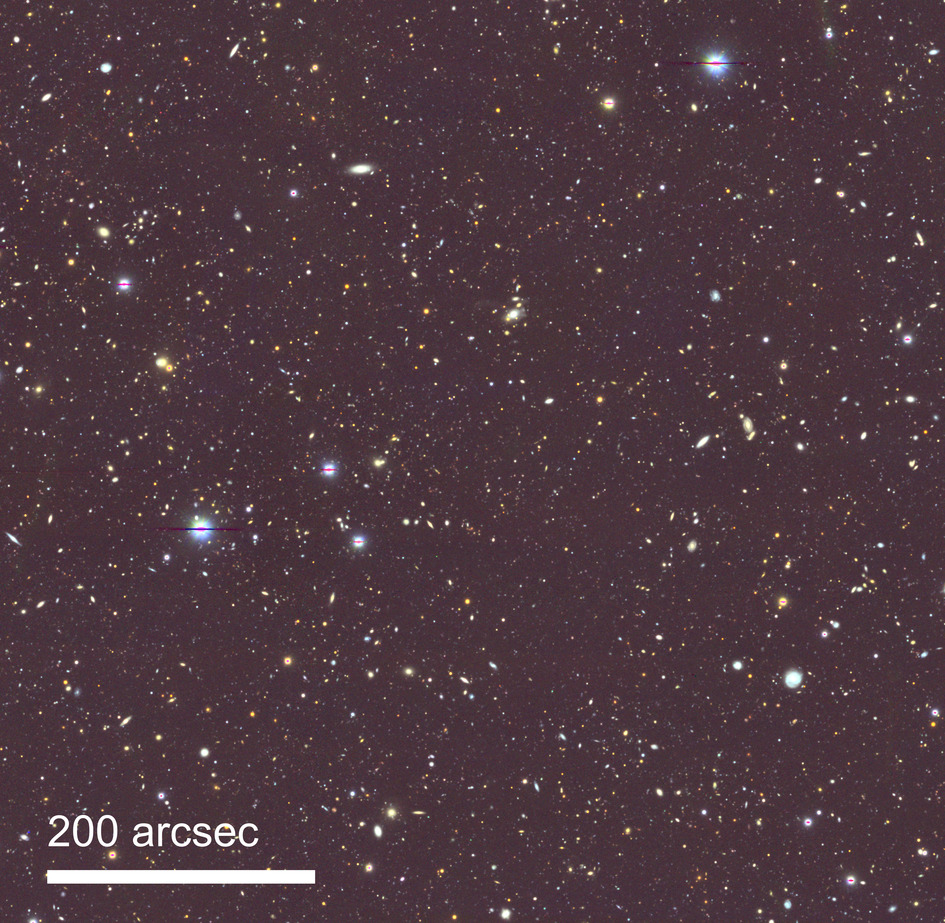
\includegraphics[width=\columnwidth]{{{fig/calexp-HSC-ZIR-9592-20.fullrgb}}}
&
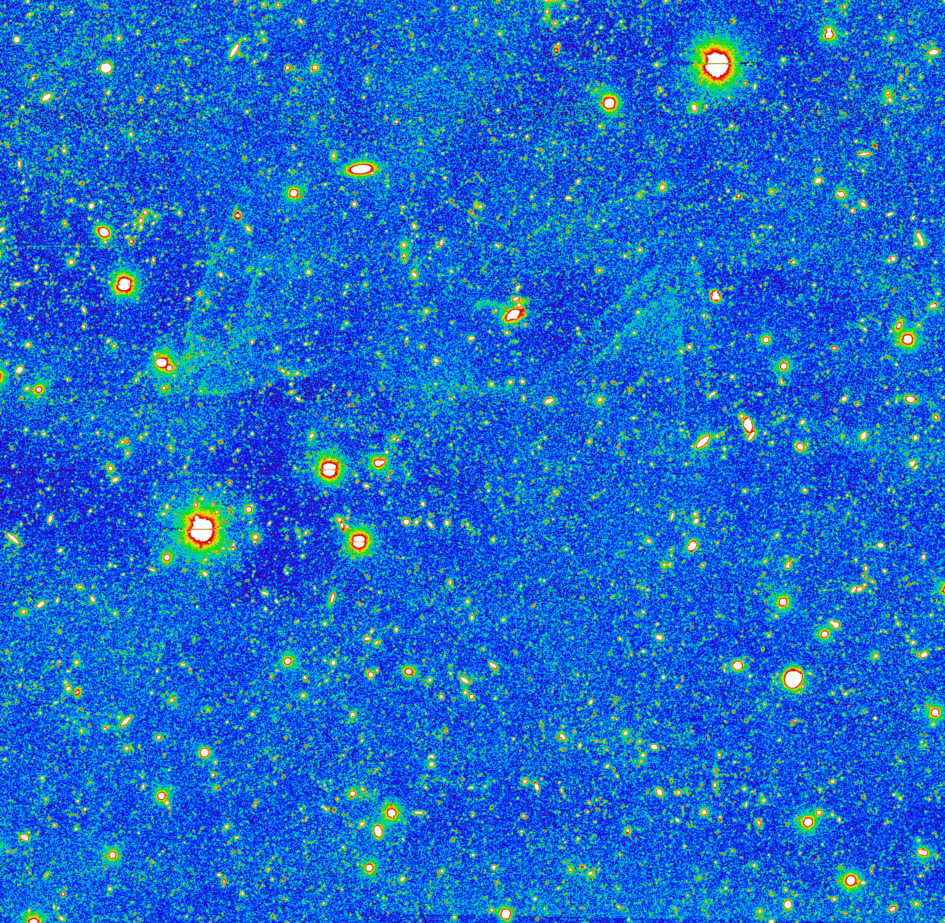
\includegraphics[width=\columnwidth]{{{fig/calexp-HSC-R-9592-20.fullmon}}}
\\\\
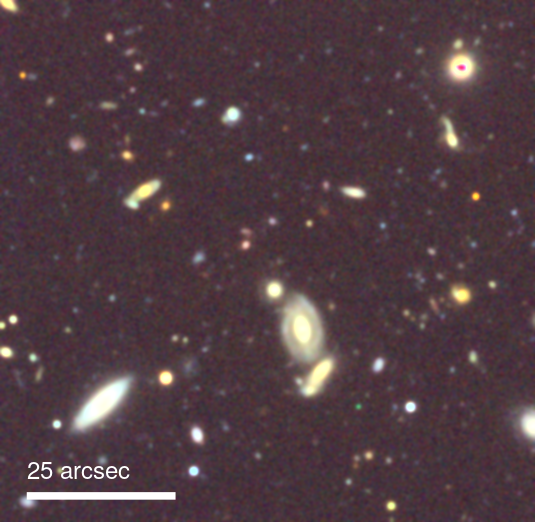
\includegraphics[width=\columnwidth]{{{fig/calexp-HSC-ZIR-9592-20.zoomrgb}}}
&
\frame{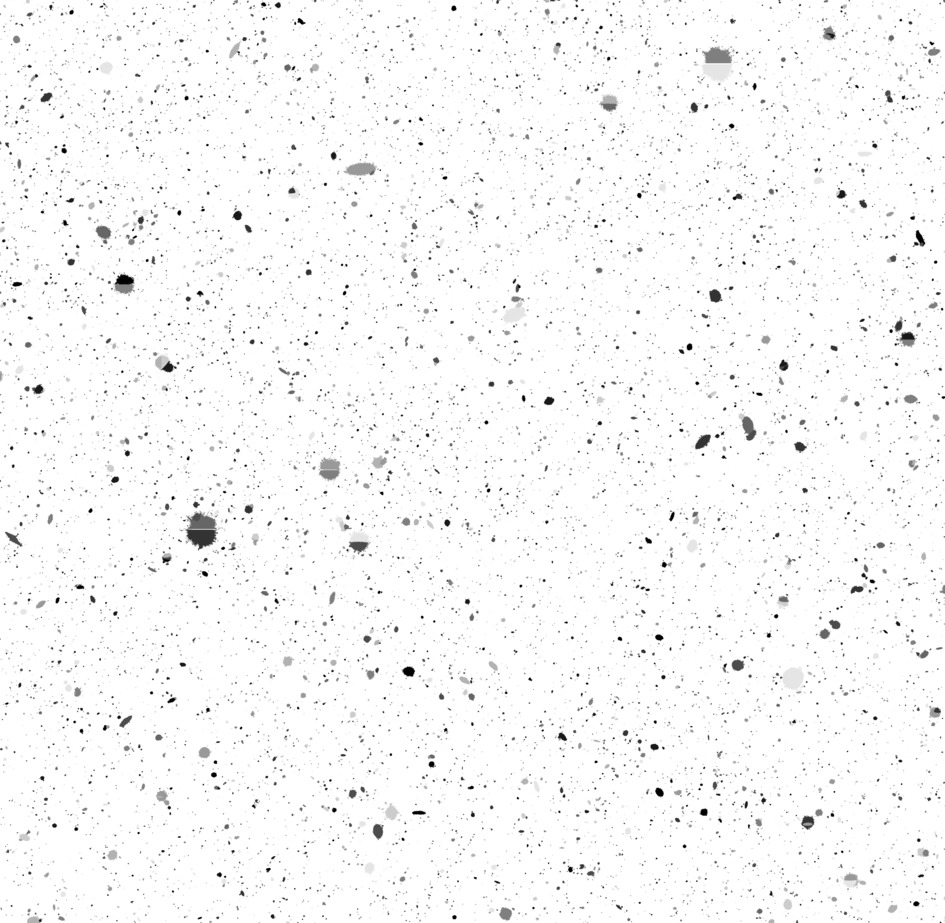
\includegraphics[width=\columnwidth]{{{fig/calexp-HSC-R-9592-20.segmap}}}}
\end{tabular}
\caption{HSC-SSP PDR1 high density region, tract-patch 9592-20. Clockwise from top left: RGB postage stamp of the entire $706\times689\;\mathrm{arcsec}$ region; $r$-band postage stamp; segmentation map; and RGB postage stamp for a $90\times88\;\mathrm{arcsec}$ zoomed cutout. All postage stamps are arctan scaled and smoothed with a Gaussian kernel of $\Gamma=3\;\mathrm{pix}$. RGB images are generated using HSC-SSP $z$, $i$ and $r$ passbands. Shades of grey within the segmentation map are randomly assigned. This high-density region will be used as a basis for the generation of a high-density simulated field.}
\label{fig:stamphi}
\end{figure*}

\subsection{Point Spread Function}
\label{sec:psf}

It is necessary to convolve our simulated images with a realistic point spread function (PSF) in order to fully account for the impact of the imaging system upon the data. We opt to generate a model of the PSF in the low density region (tract-patch 8283-38) and utilise the resultant PSF model for all subsequent simulated imaging. We use the \PSFEx \citep[][]{Bertin2011} PSF extraction software package (version 3.17.1) to generate an empirical PSF from an input \SExtractor catalogue. The \SExtractor software is operated in a similar manner to that outlined in Section \ref{sec:sample}, with the exception that the output catalogue type must be in the FITS Leiden Data Analysis Center (LDAC) file format. This file format allows for more complex data and imaging to be stored in a single entity, facilitating later PSF extraction. The columns output in this catalogue must contain: VIGNET(101,101); X\_IMAGE; Y\_IMAGE; FLUX\_RADIUS; SNR\_WIN; FLUX\_APER(1); FLUXERR\_APER(1); ELONGATION; and FLAGS. The numbers inside parenthesis following VIGNET specify the postage stamp pixel cutout size around each input point source which will ultimately be used to help define the PSF. A full description of the remaining parameters can be found in \citet{Bertin2011}, and references therein. The resultant catalogue is used as an input to \PSFEx. As with \SExtractor, \PSFEx is largely operated using its in-built defaults. Sources identified as point source like are added to a library. From our $101\times101$ pixel vignettes, we request a single output snapshot PSF of size $55\times55$ pixels in dimension. 

The \PSFEx outputs are shown in Figure \ref{fig:psf}. The top panel shows a random selection of $27$ out of a total of $424$ point sources used to construct this PSF. Nearby neighbours which may act as a flux contaminant have been automatically masked prior to use. The shape and position of these point sources on the original frame are used to construct an $\mathrm{2}^{nd}$-order polynomial model of the PSF, which is shown in the middle-left panel. This model exhibits good circular symmetry, with a measured ellipticity of $e=1-b/a\approx0.04$. Contaminant noise does become increasingly evident in the wings, however, the goodness of fit $\chi^2/\nu=0.99$ indicates a good match between the model and the input data. The empirical full-width at half-maximum is found to be $\Gamma=0.72\;\mathrm{arcsec}$. As shown in the middle-right panel, the PSF closely approximates a Moffat function down to very faint magnitudes, with fitted parameters and confidence intervals as indicated in the inset legend. The result of subtracting a scaled version of the PSF to each of the input point source samples is shown in the lower panel. The majority of point source flux is removed in the residual frame, again evidencing the high-fidelity nature of our output PSF. This PSF is used for all subsequent relevant data analysis. 

\begin{figure*}
    \centering
    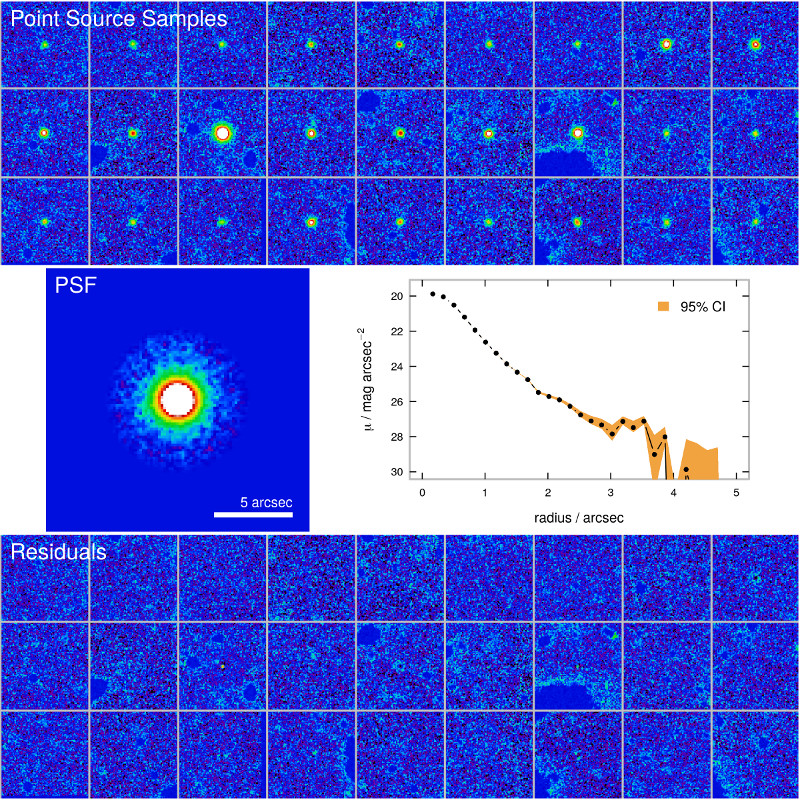
\includegraphics[width=0.9\textwidth]{{{fig/psfcheck}}}
    \caption{Visualisation of key outputs from the \PSFEx PSF modelling software, as applied to our HSC-SSP PDR1 low-density dataset (tract-patch 8283-38). Top: $27$ sample point sources, $\arcsinh$ scaled, from a total of $424$ used as an input to the PSF generation software. Middle-left: empirical PSF, log scaled, generated as the output of an $\mathrm{n}^{th}$-order polynomial fit to the shape and position of all sample point sources. Middle-right: 1D surface brightness profile of the PSF, showing the PSF data (black points), $95\%$ confidence interval (shaded orange region), and a Moffat profile fit to the observed data (purple line). Fitted Moffat parameters are shown in the inset legend. Bottom: PSF residual images, $\arcsinh$ scaled, representing the results of a flux-scaled PSF subtraction from each point source in the top panel. Much of the point source flux has been successfully removed in the residual frames, evidencing the high-fidelity nature of the output PSF model.}
    \label{fig:psf}
\end{figure*}

\section{\GalSim Simulations}
\label{sec:galsim}

\GalSim \citep{Rowe2015} is an open source software package designed to produce highly accurate simulated astronomical imaging. It has a number of powerful capabilities, including the ability to generate a broad range of galaxy and stellar profile types, perform rapid and accurate PSF convolution, and apply a physically motivated noise model. For these reasons, in addition to the speed and accuracy of the underlying base code, we opt to use the \GalSim package (version 2.2.3) to generate our simulated imaging. 

Prior to running the \GalSim software, input catalogues and associated \texttt{YAML} configuration files must be generated to specify all necessary simulation parameters. We aim to generate realistic simulated regions with noise approximating that found in HSC-SSP PDR1 data and populated with a range of objects exhibiting features similar to those found in our chosen low-density and high-density HSC-SSP PDR1 regions. Each region is exactly $4200\times4100$ pixels in dimension (approximately $706''\times689''$). For the sake of simplicity, we opt to populate these regions with extended-type \citet{Sersic1963,Sersic1968} profiles alone, avoiding the additional complication of point sources which typically contribute less to sky estimation errors (excepting the extreme bright-end population of stars) than extended profiles. Each \Sersic profile requires a total of eight input parameters: pixel position in both $x$ and $y$; total luminosity in counts; half-light radii in pixels; an axis ratio (i.e., $q = 1-e = b/a$); a position angle in degrees; a \Sersic index $n$, and; a postage stamp size in pixels. The latter of these parameters provides the edge size of a square stamp on which to draw the objects within \GalSim\footnote{Postage stamp size is not strictly required in order to generate a \Sersic profile when using \GalSim, with a default configuration available. However, for reasons which will be elucidated upon further later in this paper, we require that this parameter be specified.}. 

Input catalogues must mimic the distribution of features in the sample regions as closely as possible. A number of objects will however be missing from any detection catalogue, owing to either bright-end confusion or faint-end incompleteness. Some such parameters for these extrapolated objects require a meaningful estimation, whilst others require explicit definition. In the following sections, we provide an overview of the derivation of each required simulation parameter, concluding with a summary of our simulated field data generation. 

\subsection{Number Counts \& Magnitudes}
\label{sec:numcounts}

Perhaps the most fundamental parameter required to populate any simulated input catalogue is how many objects overall one wishes to simulate as a function of magnitude. As an initial guide, we have input catalogues for both sample regions from our initial \SExtractor runs. The solid emboldened lines in Figure \ref{fig:numcounts} show the detected number of sources per square degree and per magnitude as a function of apparent $r$-band magnitude, using a histogram bin width of $\Delta m_r=0.5$ mag. The low density region shown in the left panel, tract-patch 8283-38, contains a total of $6813$ detected sources. The high density region shown in the right panel, tract-patch 9592-20, contains a total of $12183$ detected sources. The dotted horizontal line in both panels represents the number density corresponding to one object per the area of a sample field ($\about0.038\;\deg^2$) per magnitude. 

\begin{figure*}
    \centering
    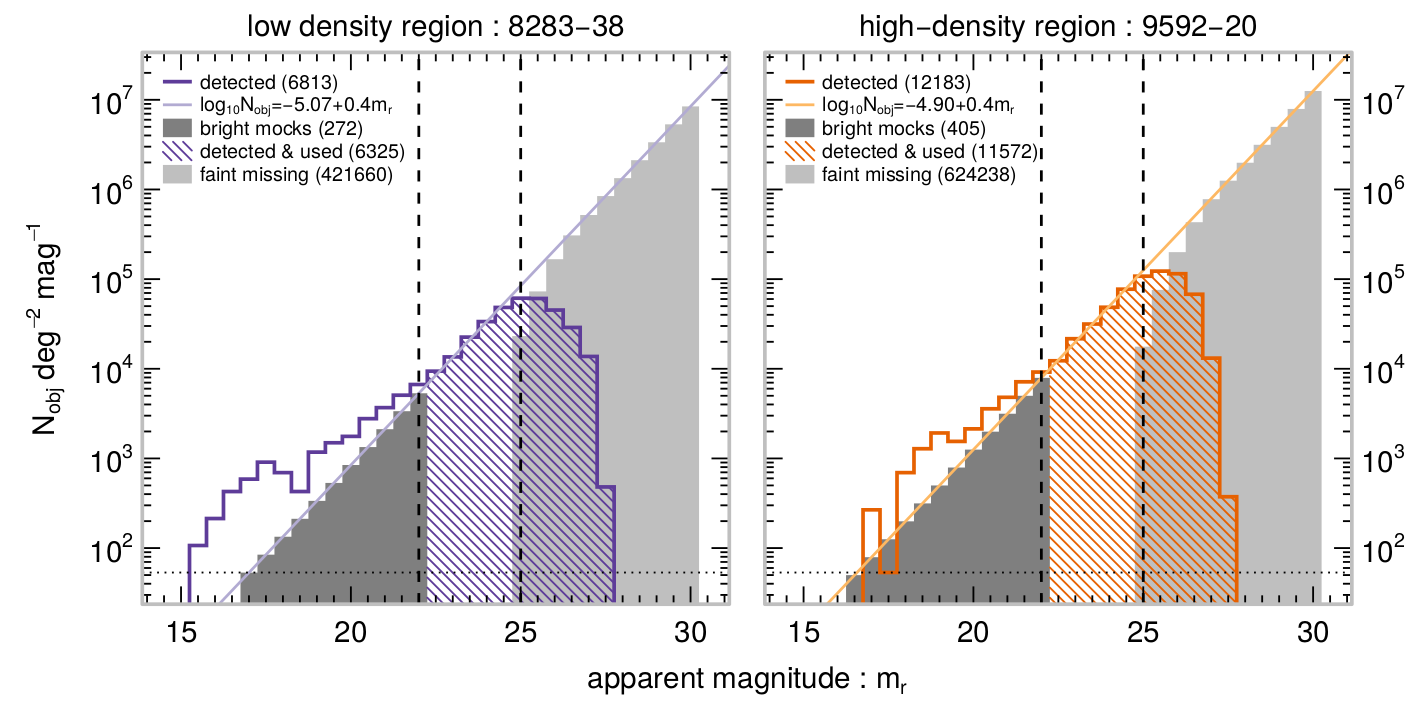
\includegraphics[width=0.9\textwidth]{{{fig/numcounts}}}
    \caption{The number of sources per square degree per magnitude as a function of apparent $r$-band magnitude. The low density region (tract-patch 8283-38) is shown in the left panel, whilst the high density region (tract-patch 9592-20) is shown in the right panel, as indicated. Within each panel, the detected source number density profile is represented as a solid emboldened line. A log-linear best fit line to the detected source profile in the range $22<m_r<25$ mag (boundaries represented by vertical dashed lines) is shown using a solid thin line. The dotted horizontal line is equivalent to one object per the area of our sample region per magnitude. Detected sources which are directly used in the simulated input catalogue (detected \& used) are found within the hatched area. Simulated sources at the bright end ($m_r<22$ mag; bright mocks) and faint end ($m_r>25$ mag; faint missing) are shown using dark grey and light grey shaded regions, respectively. These sources are defined such that their summation in addition to any relevant detected and used sources is equivalent to the fitted log-linear best fit line. Total object numbers for each regime in addition to best fit line parameters are shown in the inset legends. The three flux-associated populations defined here are used to define our input simulated number densities as a function of magnitude.}
    \label{fig:numcounts}
\end{figure*}

The brightest detected sources are found at $m_r\sim15.5$ mag in the low density region and $m_r\sim17$ mag in the high-density region. Number densities then rise in a somewhat stochastic nature down to $m_r\sim22$ mag in both fields. The fluctuations in source number density as a function of magnitude are as expected, owing to the aforementioned bright-end source confusion. In this regime, it is common for bright sources to become shredded, or for the flux in their wings to become erroneously attributed to or separated from a neighbouring source. 

The source density profile continues to rise in the magnitude range $22<m_r<25$ mag (represented by two vertical dashed lines), albeit in a log-linear fashion. A constrained log-linear fit to the detected source density profile in this regime is represented as a solid thin line in both panels. Following \citet{Ji2018}, the slope of this best fit line is kept fixed, with only the intercept parameter fitted. We find the low density regime source density profile goes as $\log_{10}N_{\mathrm{obj}}=-5.07+0.4m_r$. The high density regime source density profile goes as $\log_{10}N_{\mathrm{obj}}=-4.90+0.4m_r$. 

At magnitudes fainter than $m_r\sim25$ mag, detected source densities begin to turn down, dropping off completely by $m_r\sim28$ mag. Such faint-end incompleteness is inherent in any source detection catalogue, as sources gradually become indistinguishable from the background noise and instead contribute to the faint undetected EBL. 

Detected sources brighter than $m_r=22$ mag are significantly more numerous than that predicted by our best fit log-linear trend line, occasionally by almost an order of magnitude. It would be unwise to use these catalogue entries when defining a simulated input catalogue if indeed these sources are erroneously shredded sub-components of larger singular sources. We opt to discard all detected sources brighter than $m_r=22$ mag and use the best fit trend line to define a replacement bright end dataset in its place. New bright mock sources are distributed uniformly within each $\Delta m_r=0.5$ mag bin. This procedure produces a total of $272$ new sources in the low density region and $405$ new sources in the high density region. 

Remaining detected sources at intermediate and faint magnitudes are relatively free from such source processing issues. A single object detected in the low density region exhibited an erroneous flux value, and is consequently removed from all subsequent analyses. We therefore opt to propagate $6325$ such objects through to our simulated input catalogue from the low density region, and $11572$ from the high density region. 

To account for known faint end incompleteness, we additionally derive a population of faint missing sources in the range $25<m_r<30$ mag. These sources are defined as the population required in addition to any detected and used sources which would satisfy our best fit log-linear source density trend line. As with the bright mock sources, these new faint sources are distributed uniformly within each $\Delta m_r=0.5$ mag bin. As such, this provides an additional $421660$ faint end sources in the low density region, and $624238$ faint end sources in the high density region. 

In summary, we have defined three distinct flux-associated source populations: bright mock sources, intermediate-brightness detected and used sources, and faint missing sources. These three populations are propagated through to our simulated catalogue and are represented in Figure \ref{fig:numcounts} as dark grey, hatched, and light grey shaded regions, respectively. In total, we simulate $428257$ sources in the low density regime, and $636215$ sources in the high density regime. Magnitudes are converted to counts using the standard HSC-SSP \texttt{deepCoadd\_calexp} zero point magnitude of $27.0\;\mathrm{mag}\;\mathrm{ADU}^{-1}$ \citep{Aihara2018b}.

\subsection{Half Light Radii}
\label{sec:magradii}

It's necessary and desirable for our simulated source sizes to mimic as closely as possible the distribution of size as a function of magnitude found in our observed data. The preliminary source detection catalogues provide half light radii for our chosen intermediate brightness detected \& used sources; a starting point upon which to generate an appropriate size-magnitude distribution. Some form of extrapolation is however required to provide radii for the remaining brighter/fainter simulated source populations as outlined in Section \ref{sec:numcounts}. 

Figure \ref{fig:magradii} shows recovered half light radii as a function of apparent $r$-band magnitude for all extended-type detected sources in both the low-density region (orange data points) and high-density region (purple data points). We define extended-type sources as those with a \SExtractor stellar classification parameter in the range $\mathrm{CLASS\_STAR}<0.05$, removing obvious point sources. The application of this cut removes $386$ of $18995$ potential sources. Despite making this cut, two remnant point source spurs are evident at $r_{e,\mathrm{low}}\approx0.5$ and $r_{e,\mathrm{high}}\approx0.3$, with the low density region PSF evidently more extended than its high density region equivalent. The apparent bias in half light radius at any given magnitude as a function of field density is due to this effect, with sources in the low density regime (orange data points) appearing consistently larger on average by a factor of $\about2$ than their equivalent-brightness sources in the high density regime (purple data points). 

\begin{figure}
    \centering
    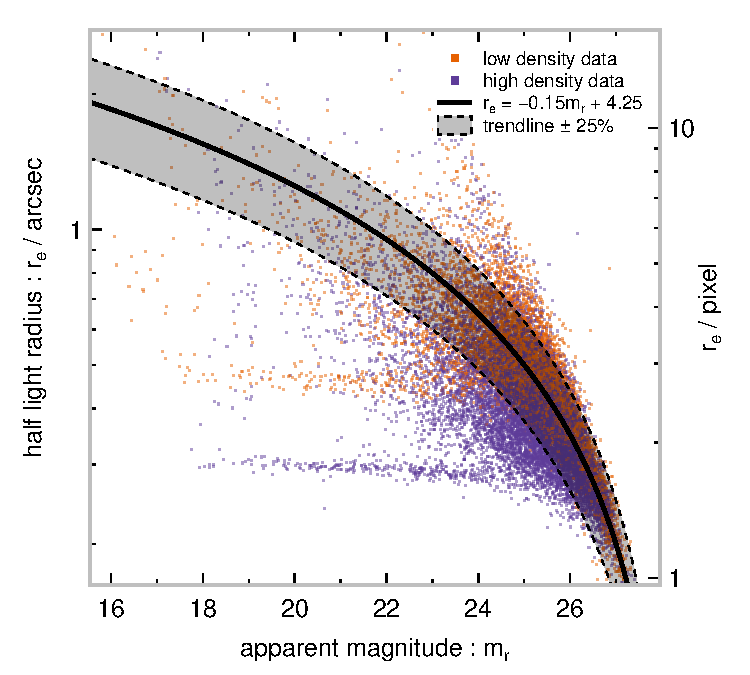
\includegraphics[width=\columnwidth]{{{fig/magradii}}}
    \caption{Recovered half-light radii as a function of apparent $r$-band magnitude for all extended-type ($\mathrm{CLASS\_STAR}<0.05$) detected sources. Sources from the low density region are shown in orange, whilst sources from the high density region are shown in purple. The solid bold black line represents a best fit trendline to those extended-type sources brighter than $m_r=22.25$ mag. Simulated bright mock and faint missing sources are randomly distributed within the $\pm25\%$ boundaries about this trendline down to an absolute minimum of $1$ pixel.}
    \label{fig:magradii}
\end{figure}

We fit a linear trendline to all detected extended-type sources brighter than $m_r=22.25$ mag using the \texttt{lm} linear minimisation routine \citep{Chambers1992} within the \textsc{R} programming language \citep{RCoreTeam}. The fit is constrained in order to accurately model the bulk population trend. We find a best fit line given by the equation $r_\mathrm{e}=-0.15m_r+4.25$, represented in Figure \ref{fig:magradii} as a solid bold line. Dashed lines bounding the shaded grey region represent the trend radius $\pm25\%$. We use this relation, alongside simulated bright mock and faint missing $r$-band magnitudes, to estimate simulated half light radii. Simulated radii are randomly uniformly distributed within the $\pm25\%$ boundary at a given magnitude down to an absolute minimum of $1$ pixel $\pm25\%$ (i.e., the faintest simulated source half light radii are randomly uniformly distributed in the range $[0.75,1.25]$ pixels). 

\subsection{Ellipticities}
\label{sec:magellip}

As with radii in Section \ref{sec:magradii}, simulated ellipticities (where $e=1-b/a$) are likewise based upon our combined low/high density preliminary detected source catalogues. Figure \ref{fig:magellip} shows median ellipticities according to the inset colour legend in bins of half light radius along the $y$ axis and apparent $r$-band magnitude along the $x$ axis. The top panel shows our observed (detected) extended-type dataset, whilst the bottom panel shows our resultant extrapolated modelled (simulated) ellipticity dataset. Apparent magnitude data along the $x$ axis is binned into $0.5$ mag bins (see Figure \ref{fig:numcounts}). Half light radii are subdivided into quartiles, thereby covering the full gamut of radii within each magnitude bin. For example, median half light radii at $m_r=21$ mag are $0.46''$ at $Q1$, $0.69''$ at $Q2$, $0.85''$ at $Q3$ and $1.04''$ at $Q4$, whilst median half light radii at the fainter $m_r=27$ mag are $0.19''$ at $Q1$, $0.21''$ at $Q2$, $0.23''$ at $Q3$ and $0.25''$ at $Q4$. Regions enclosed within a solid black outline in the observed (detected) top panel show those bins containing $25$ or fewer sources (equating to a total of $270$ sources from a potential $18609$). As shown, the general trend is for larger objects to be more elliptical (less circular) at all magnitudes. Ignoring minimally occupied bins, we find a trend for detected sources becoming more circular as one progresses from bright magnitudes down to $m_r\approx23$ mag. Continuing on to fainter magnitudes reverses this trend, with median source ellipticities becoming more elliptical once more, culminating with one of the highest overall median ellipticity bins at $m_r=27$ mag. 

\begin{figure*}
    \centering
    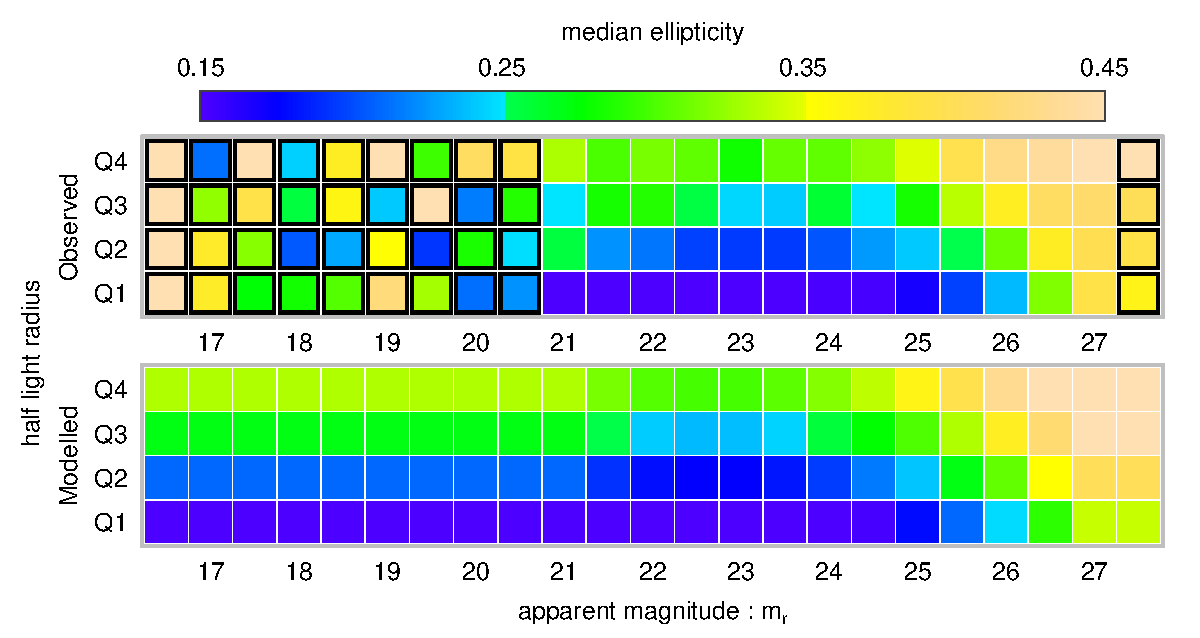
\includegraphics[width=0.9\textwidth]{{{fig/magellip}}}
    \caption{Median ellipticities in bins of half light radii and apparent $r$-band magnitudes. Observed (detected) extended-type data is shown in the top panel, modelled (simulated) data is shown in the bottom panel. Observed bins enclosed within a solid black square represent minimally occupied bins containing $25$ or fewer sources. A fit to all remaining bins with $25$ or more sources each is used to construct the model in the lower panel (see text for more details).}
    \label{fig:magellip}
\end{figure*}

All observed (detected) bins containing $25$ sources or more per bin (those without a surrounding solid black outline in Figure \ref{fig:magellip} in the magnitude range $21<m_r<27$ mag) are used to define a model fit to this feature space. Those bins containing $25$ or fewer sources exhibit a relatively large scatter on recovered median ellipticity, necessitating their exclusion here. The \texttt{lm} minimisation routine is used to fit a multi-dimensional model, with a best fit output given by:
\begin{equation}
    \label{eq:magellip}
    \tilde{e} = 6.31564 + 0.06165\,r_{e,Q} - 0.55233\,m_r + 0.01217\,m_r^2
\end{equation}
where $\tilde{e}$ is the median ellipticity for a given bin, $r_{e,Q}$ is the half light radius quartile bin number (namely: $1$, $2$, $3$, or $4$) and $m_r$ is the bin apparent $r$-band magnitude. This model is applied directly in the magnitude range $21<m_r<27$ mag, i.e., those magnitudes containing well-populated bins in Figure \ref{fig:magellip}. In order to avoid the perils of Runge's phenomenon when extrapolating this model to the extreme limits of magnitude employed here, we opt to directly map model median ellipticities from the $m_r=21$ mag bin on to each bin in the range $m_r\leq20.5$ mag. Similarly, we opt to directly map model median ellipticities from the $m_r=27$ mag bin on to each bin in the range $m_r\geq27.5$ mag. This procedure defines the model shown in the lower panel of Figure \ref{fig:magellip}. Bright mock sources are assigned a simulated ellipticity given their simulated input half light radius and magnitude according to this model, with ellipticities randomly uniformly assigned in the range $\pm0.2$ about their modelled median ellipticity. Intermediate-brightness sources which are detected and used propagate their detected ellipticities directly. Following the trend in our faintest magnitude bin, faint missing sources are randomly uniformly assigned an ellipticity in the range $0.4\pm0.2$.

\subsection{Position Angles}
\label{sec:positionangle}

Associated with ellipticity is the position angle along which to align the source major axis. We opt to propagate position angles for those intermediate brightness detected and used sources directly into the simulated input catalogue. All remaining bright mock sources and faint missing sources are randomly uniformly assigned a position angle in the range $-90<\mathrm{P.A.}<90$ degrees. 

\subsection{Locations within the Field}
\label{sec:pixelposition}

One of the most fundamental parameters required as an input to \GalSim is at what position along $x$ and $y$ should the simulated source be placed. We have three varying brightness datasets: bright mock; intermediate-brightness detected and used, and; faint missing, with each requiring a different positional prescription. The simplest is for intermediate brightness detected and used source positions, which are propagated directly into the final simulated catalogue. Faint missing sources are extremely numerous, with around half a million simulated sources injected into both sample regions. Owing to their significant abundance, we opt to randomly uniformly assign faint missing source position centroids along the $x$ axis in the range $0.5<x<4200.5$ pixels. Half-pixel start and end points reflect the \texttt{FITS} convention that the centre of the lower left corner pixel has the coordinate $[1,1]$ and a width of $1$ pixel. As with the $x$ axis, pixel position centroids along the $y$ axis are similarly randomly uniformly assigned in the range $0.5<y<4100.5$ pixels. 

The top two panels of Figure \ref{fig:hireslores} show arctan scaled full resolution images for our low density region (left) and high density region (right). As is evident, several bright sources may on occasion cluster together to form a loose group. Whether a `true' group in three-dimensional space or a mere projection effect, the resulting flux bridges that link these sources on the sky leave that region prone to sky over-subtraction effects. Any investigation of this effect must therefore place bright simulated sources in such a way so as to preserve any clustering signature. We use these input datasets as a basis for determining such signatures. The lower two panels in Figure \ref{fig:hireslores} show artificially degraded low resolution versions of their full resolution counterparts, with the low density region on the left and the high density region on the right. Each axis in the full resolution image is split into $100$ `super pixels', resulting in $4200/100=42$ super pixels along the $x$ axis and $4100/100=41$ super pixels along the $y$ axis. The mean flux value for each super pixel (equating to $42\times41=1722$ ordinary pixels) is calculated, resulting in the low resolution images shown here. 

\begin{figure*}
    \centering
    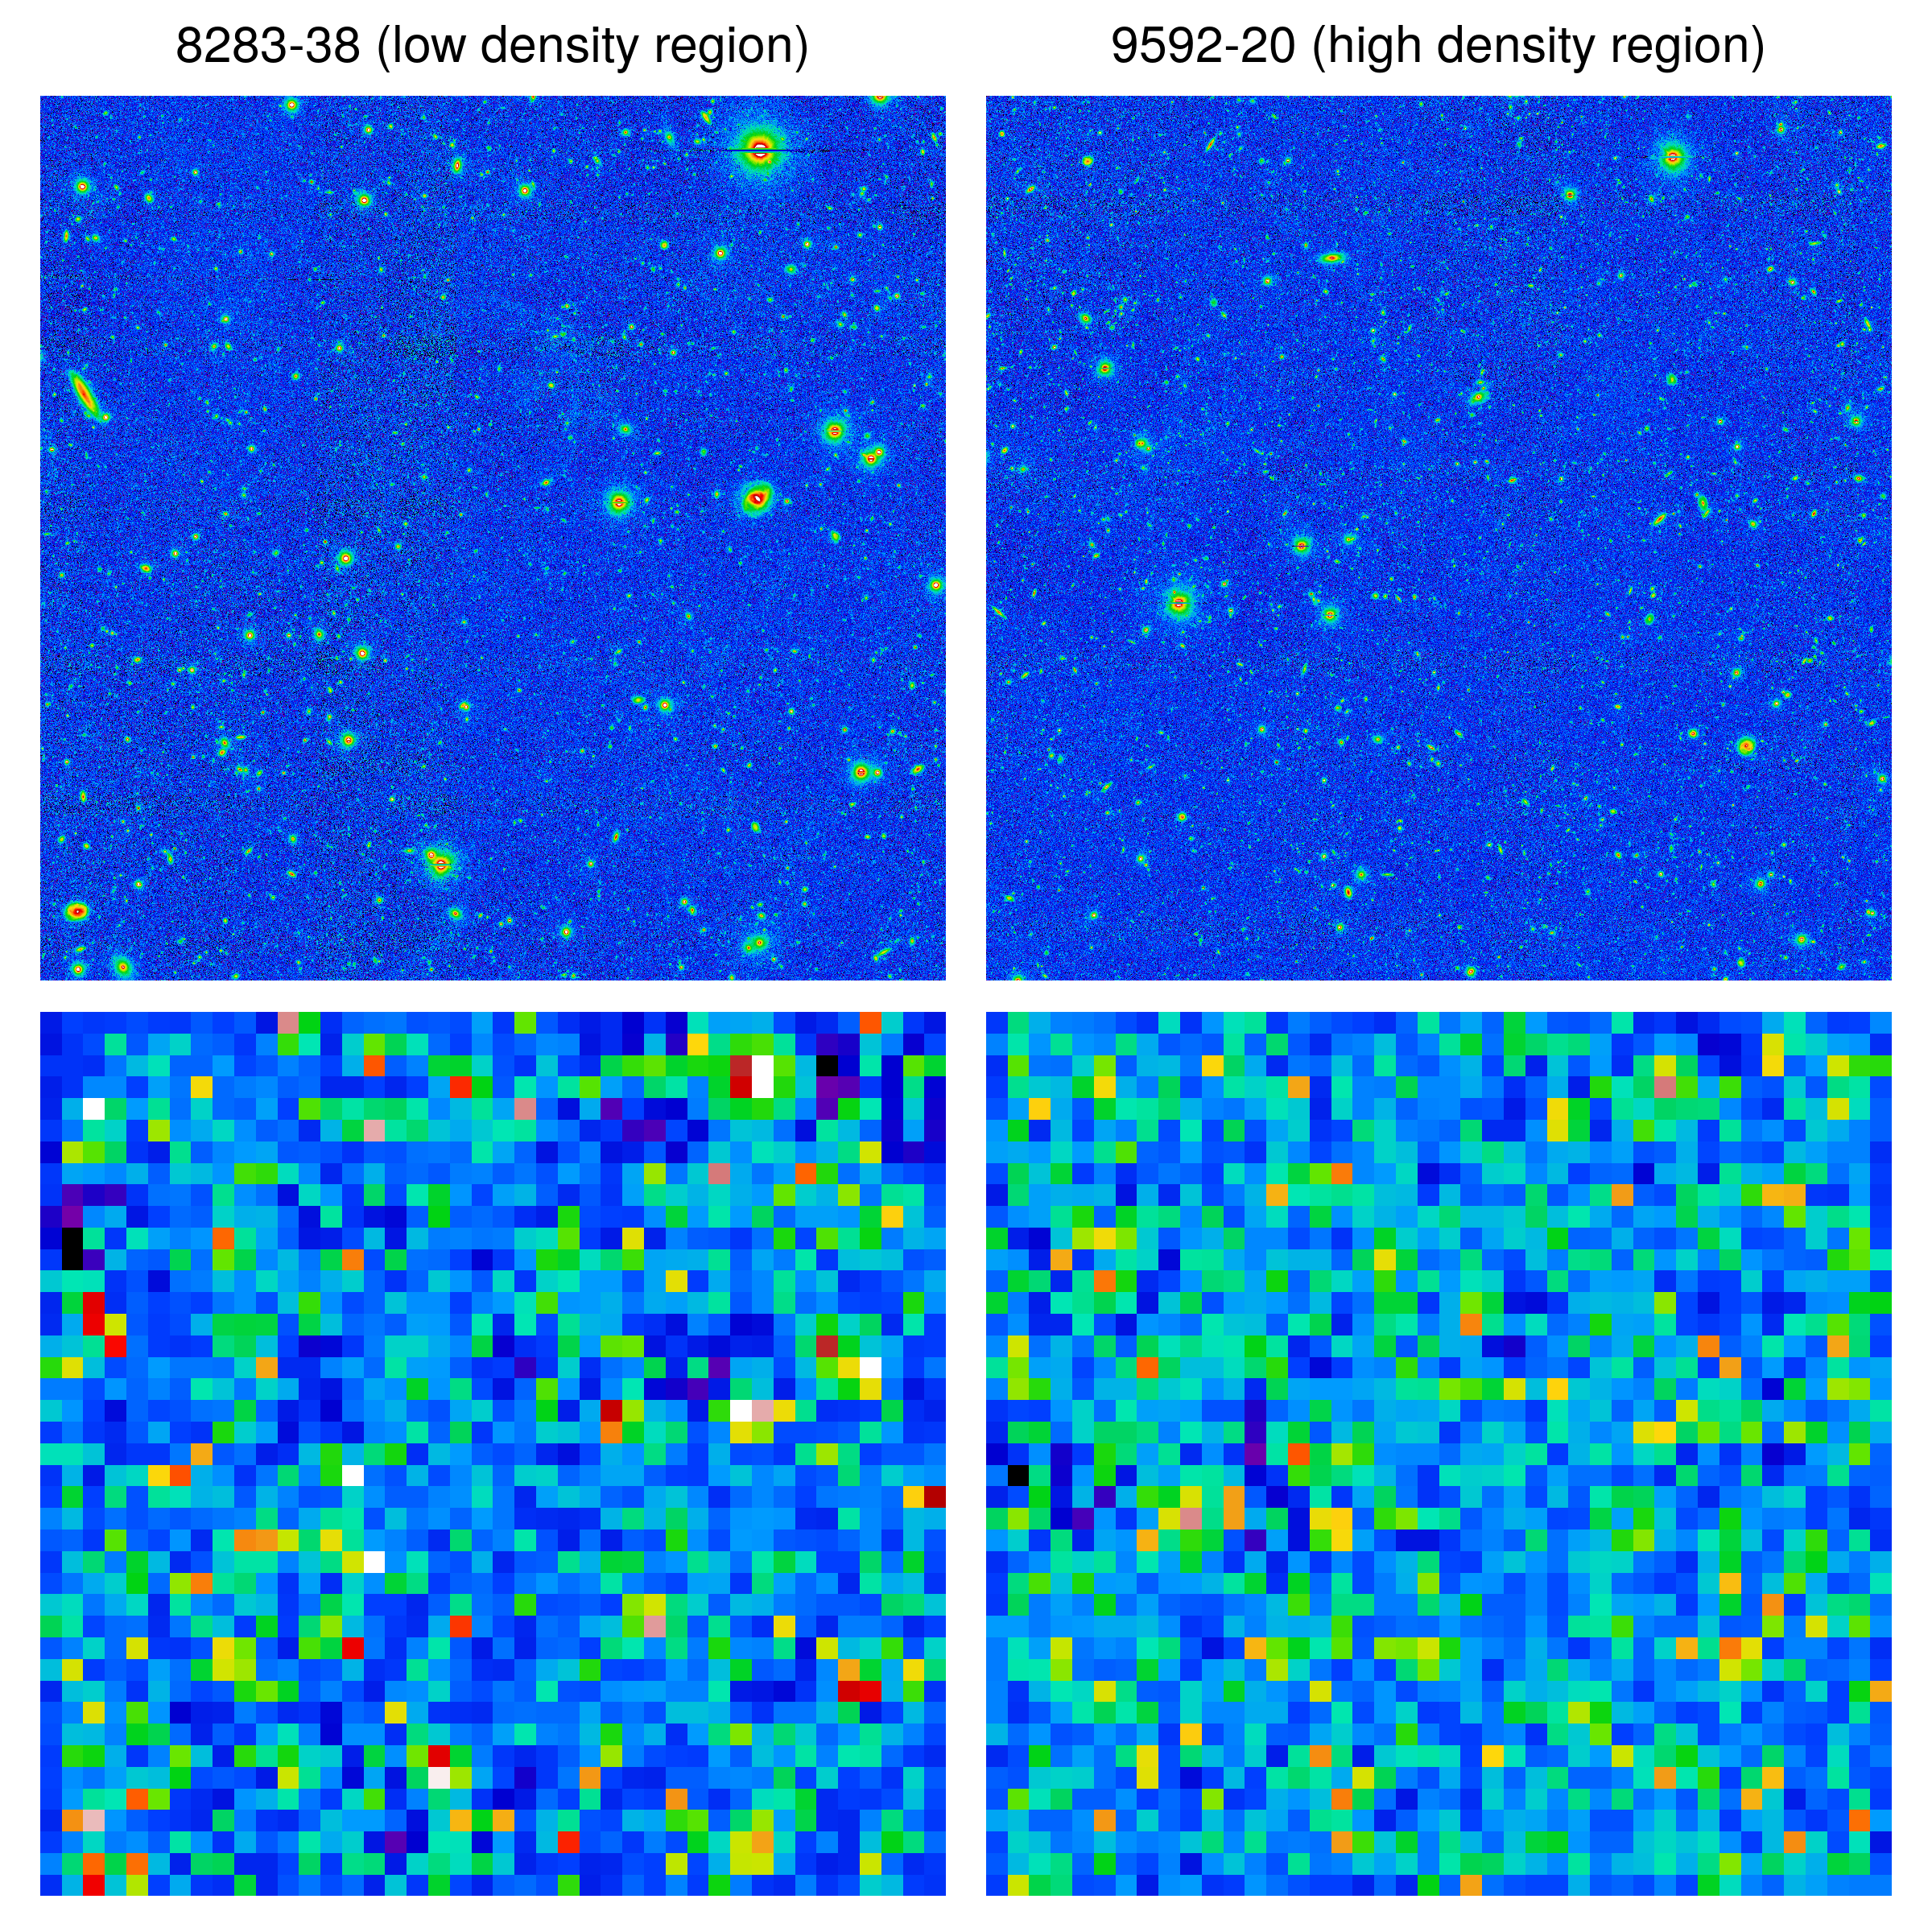
\includegraphics[width=0.9\textwidth]{{{fig/hireslores}}}
    \caption{HSC-SSP PDR1 full-resolution (top) and artificially degraded low-resolution (bottom) imaging for both sample regions: low density on the left and high density on the right. Images are arctan scaled. Full resolution images are smoothed with a Gaussian kernel of $\Gamma=3\;\mathrm{pix}$ prior to plotting. Each super pixel in the low resolution image is a mean of $42\times41=1722$ ordinary pixels in the original data. Low resolution images are used to define a weight function when determining bright mock source centroid placement.}
    \label{fig:hireslores}
\end{figure*}

To preserve any clustering signature in our sample regions, low resolution imaging is used to define a positional weight function. A weight map is constructed by rescaling the low resolution images on to the range [$0.0\rightarrow1.0$]. Bright mock sources are iteratively assigned a randomly weighted position using the \texttt{sample} routine within \textsc{R} \citep{Ripley1987}. 

\subsection{\Sersic Indices}
\label{sec:sersicindex}

Owing to the well known bimodality in galaxy radial profiles \citep{Baldry2004,Baldry2006,Driver2006,Kelvin2012,Kelvin2014a,Kelvin2014b,Taylor2015}, we opt to simulate \Sersic-like galaxies with \Sersic indices of $n=1$ (i.e., exponential disk-like) and $n=4$ (i.e., de Vaucouleurs type spheroid-like). Each simulated region is simulated twice, with each simulated source given a \Sersic index of $n=1$ and, separately, a \Sersic index of $n=4$. Simulating disk-like and spheroid-like sources allows us to explore the accuracy of our sky-estimation routine as a function of source profile type, with de Vaucouleurs sources exhibiting significantly more flux in their outer wings than their exponential counterparts. 

\subsection{Postage Stamp Cutout Sizes}
\label{sec:postagestamps}

Postage stamp size is the final required per-object \GalSim input parameter. Each simulated source generated by \GalSim is extrapolated out to the limits of a user-provided box, known as the postage stamp. This limitation exists for reasons of computational efficiency, notably in reducing the number of pixels requiring PSF convolution. A-priori knowledge of all relevant \Sersic parameters (magnitude, half-light radius, \Sersic index and ellipticity) allows us to determine the surface brightness drop-off as a function of semi-major axis radius for each simulated source. We opt to define postage stamp boxes for each source such that a source aligned parallel to the $x$-axis would reach a surface brightness limit of $\mu_r=35\,\mathrm{mag}/\mathrm{arcsec}^{-2}$ at the boundary of the postage stamp. This limit is sufficiently faint to facilitate exploration of the background sky, yet not too deep to preclude the construction of these simulated frames. A minimum postage stamp size of $11\times11$ pixels is enforced\footnote{This postage stamp size limit is reached only in the exponential $n=1$ case for $\about12\%$ of sources.}. See Section \ref{sec:postagestampsizes} for further discussion on the importance of choosing an appropriate postage stamp cutout size.

\subsection{Gain and Sky Level}
\label{sec:gainskylevel}

To ensure that output simulated imaging exhibits Poisson noise which mimics that found in coadded sky-subtracted HSC-SSP PDR1 data, \GalSim requires as an input the mean detector gain and an estimate of the original average sky level pedestal. Averaged equivalent gains (in units of electrons per count) are provided and trivially extracted from the \texttt{FITS} headers of HSC-SSP mosaicked imaging. Unfortunately however, for these PDR1 data, subtracted background sky maps are not provided, nor is an easily accessible record kept of subtracted sky levels. Consequently, we perform a basic estimate of the initial sky level based upon the root mean square (RMS) of the flux in those pixels identified as background. Given an averaged equivalent gain $g$ and a measure of background RMS flux from our initial \SExtractor runs across both density regimes, we estimate the original sky level $f_\mathrm{sky}$ in $\mathrm{counts}/\mathrm{pixel}$ using the relation $f_\mathrm{sky}=g\cdot\mathrm{RMS}^2$. Using this relation, in the low density regime (8283-38) we find $g=557.9\,e^{-}/\mathrm{count}$ and $f_\mathrm{sky}=1.645\,\mathrm{counts}/\mathrm{pixel}$, whilst in the high density regime (9592-20) we find $g=563.9\,e^{-}/\mathrm{count}$ and $f_\mathrm{sky}=1.391\,\mathrm{counts}/\mathrm{pixel}$.

\subsection{\GalSim Setup}
\label{sec:galsimsetup}

The above sections detail the generation of all required \GalSim input parameters. With these parameters defined, input catalogues for all regions of interest are constructed. Input catalogues contain positional information alongside all other parametric variables required to construct a \Sersic model for each simulated source (see Section \ref{sec:inputcats} for further details).

We aim to fully explore the accuracy of various background subtraction techniques as a function of field density, source profile shape and background light contamination. In addition to two density regimes (low and high as defined in Section \ref{sec:sample}, termed here as `denlo' and `denhi', respectively) and two profile types ($n=1$ and $n=4$, see Section \ref{sec:sersicindex}), we also define a bright-end flux subset of the data. This allows us to explore the performance of sky subtraction algorithms with a known removal of faint undetected components, the primary contributors to EBL. Three simulated populations roughly segregated by flux are defined in Section \ref{sec:numcounts}: bright mock sources ($m_r<22$ mag), intermediate brightness detected and used sources ($m_r>22$ mag, becoming increasingly incomplete fainter than $m_r=25$ mag) and faint missing sources (i.e., known missing sources in the range $m_r>25$ mag). We define a `bright' sample as the combination of those simulated sources belonging to the first two of these simulated populations, i.e., bright mock sources and intermediate brightness detected and used sources. From the initial $428257$ simulated sources in the low density regime and $636215$ simulated sources in the high density regime, this bright end cut extracts $6597$ low density region sources and $11977$ high density region sources. Taken together, we generate a total of eight simulated regions. These regions are summarised in Table \ref{tab:simtab}.

\begin{table}
    \setlength{\tabcolsep}{5pt}
    \begin{tabular}{ l | l | l | l | l }
    label & based on & flux subset & source density & \Sersic index\\
    \hline
    denlo1a & 8283-38 & all & low & 1\\
    denlo4a & 8283-38 & all & low & 4\\
    denhi1a & 9592-20 & all & high & 1\\
    denhi4a & 9592-20 & all & high & 4\\
    denlo1b & 8283-38 & bright & low & 1\\
    denlo4b & 8283-38 & bright & low & 4\\
    denhi1b & 9592-20 & bright & high & 1\\
    denhi4b & 9592-20 & bright & high & 4\\
    \end{tabular}
    \caption{A summary table providing an overview of our final eight simulated regions. From left to right, columns are: a short label for this simulated dataset; the input HSC-SSP PDR1 tract-patch ID upon which this simulated data is based; the flux population subset; the relative source density of the region; and, the \Sersic index assigned to each simulated source in that region. Flux population subset is either `all' (i.e., all simulated sources as outlined in Section \ref{sec:numcounts}) or `bright'. This `bright' flux subset identifier indicates that the `faint missing' sources described in Section \ref{sec:numcounts} have been excluded from this simulation, thereby limiting it to the `bright mock' and `intermediate detected and used' simulated sources. }
    \label{tab:simtab}
\end{table}

Input catalogues for each simulated frame defined in Table \ref{tab:simtab} are constructed. An associated YAML `feedme' configuration file is also generated specific to each simulated region. This configuration file specifies input and output filenames, defines the PSF and \Sersic components and assigns global parameters. For further information see Section \ref{sec:yamlconfig} and \citet{Rowe2015}. 

\subsection{Simulated Fields}
\label{sec:simfields}

The \GalSim software package is run across each simulated field defined in Table \ref{tab:simtab}. The figures below show the results of these runs. Figure \ref{fig:simstampfulllo} shows all four simulated outputs for the low density `denlo' region. All simulated \Sersic sources are convolved with an empirical PSF, and realistic Poisson noise has been added commensurate with typical HSC-SSP PDR1 data. The background is set to zero in all of these simulations. The top left panel shows the full simulated field populated exclusively with exponential $n=1$ disk-like components. The top right panel shows the equivalent full simulated field populated exclusively with de Vaucouleurs type $n=4$ spheroid-like components. The bottom left and bottom right panels also show the $n=1$ and $n=4$ fields, respectively, yet only for the bright flux sub-population as defined in Section \ref{sec:galsimsetup} (i.e., bright mocks and intermediate brightness detected and used sources). The scale inset into the top left panel applies equivalently to all panels. 

\begin{figure*}
    \centering
    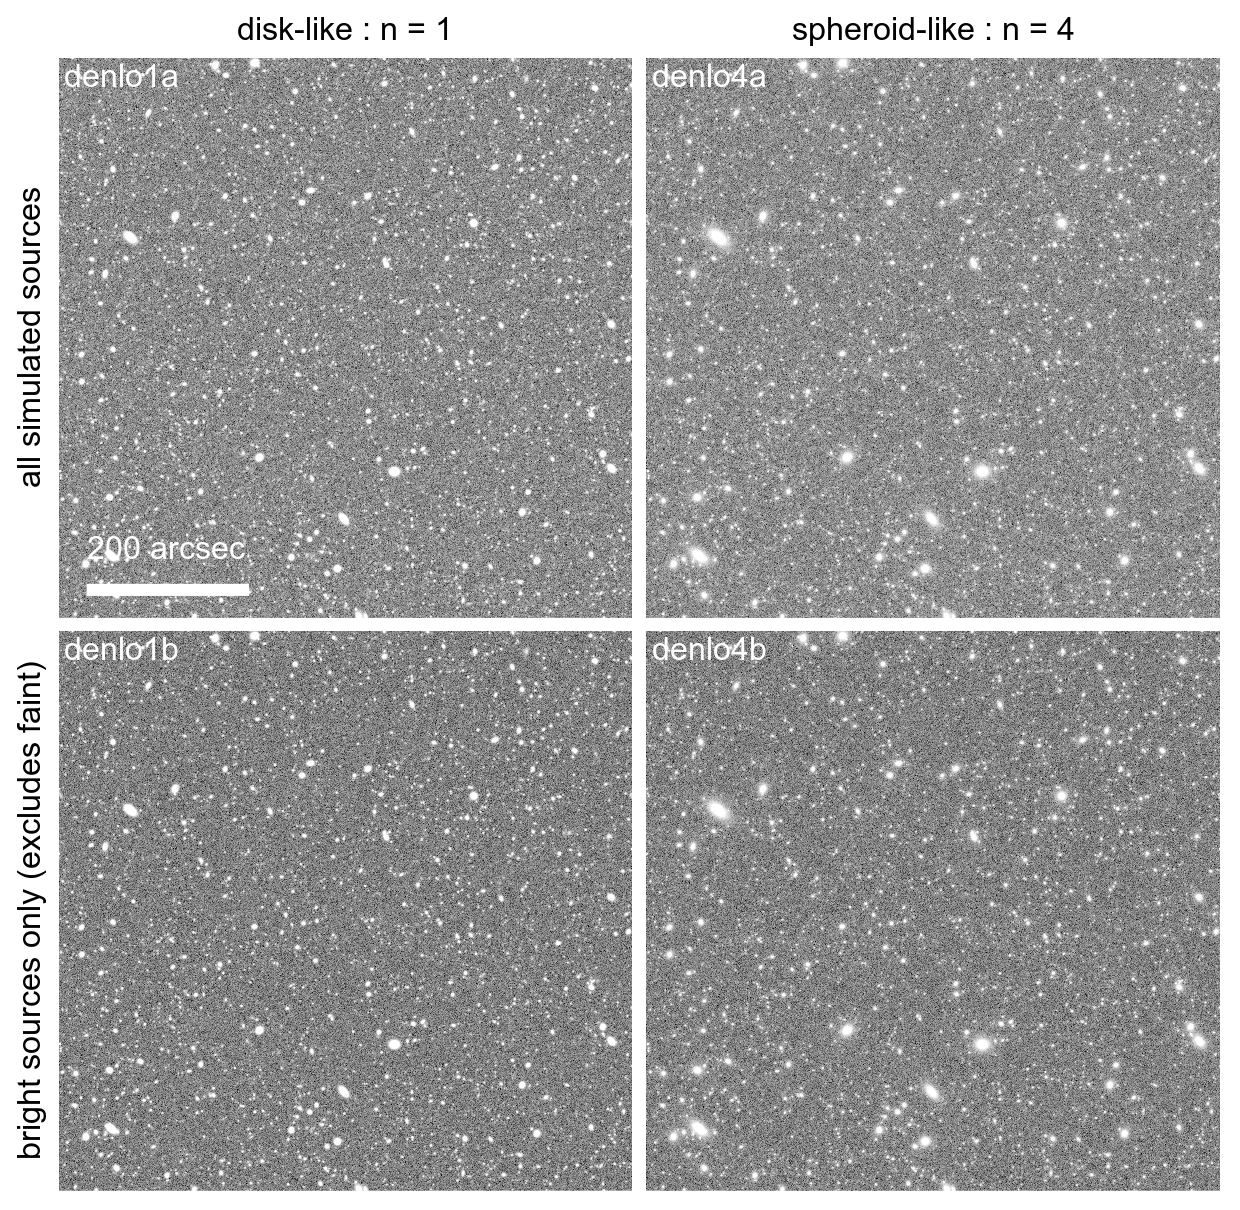
\includegraphics[width=0.9\textwidth]{{{fig/simstamp-full-8283-38}}}
    \caption{All four \GalSim simulated outputs for the low density `denlo' region. Top left: The full simulated low density field populated exclusively with exponential $n=1$ disk-like sources. Top right: The full simulated low density field populated exclusively with de Vaucouleurs $n=4$ spheroid-like sources. Bottom left: The bright end sub-population only (i.e., excluding faint missing sources), with each source described by an $n=1$ \Sersic profile. Bottom right: The bright end sub-populations only, with each source described by an $n=4$ \Sersic profile. The scale inset into the top left panel applies equivalently to all panels. All sources are PSF-convolved, and HSC-SSP PDR1 Poisson noise has been added. Images are arctan scaled. The impact of source population (i.e., contrasting the top row with the bottom) and source profile type (contrasting the left column with the right) is visibly evident on the apparent background level.}
    \label{fig:simstampfulllo}
\end{figure*}

As can be seen, the absence of EBL in the lower two panels marks them as visually distinct from their full simulated counterparts in the upper panels, with the background sky in the bright-only panels notably lower. Further, the extended $n=4$ \Sersic profiles in the two right side panels appear to visibly contaminate a relatively larger fraction of the background sky than equivalent exponential type sources do. Both such factors are potentially significant contributors to inaccurate background sky estimation, and require careful consideration. 

Figure \ref{fig:simstampzoomlo} is configured similarly to Figure \ref{fig:simstampfulllo}, but zoomed in on a particular region of interest as shown by the inset legend. Here it becomes apparent that the brightest of the faint background sources present in the full simulated data appear as faint fuzzy patches scattered across the sky. Such sources are notably missing in the bright only simulations. Their form bears a striking similarity to many such objects recorded throughout the literature, notably: the `small condensed galaxy' in \citet{Arp1965}; the `dwarf galaxies' of \citet{Sandage1984}; the `compact galaxies' in \citet{Guzman1997}; the `little blue fuzzies' of \citet{Brough2011}; the `green peas' of \citet{Cardamone2009,Bauer2013}; the `little blue spheroids' defined in \citet{Kelvin2014a,Kelvin2014b}; `low surface brightness galaxies' in \citet{Williams2016}; and, the `ultra diffuse galaxies' of \citet{vanderBurg2016}, amongst others. Further, automated classification algorithms are now identifying and characterising such sources on an increasingly regular basis, as in, e.g., \citet{Sreejith2018,Turner2019}, with possible formation mechanisms outlined in \citet{Stinson2007}. As noted above, these systems may potentially significantly affect background sky estimation procedures, and therefore require further study. 

\begin{figure*}
    \centering
    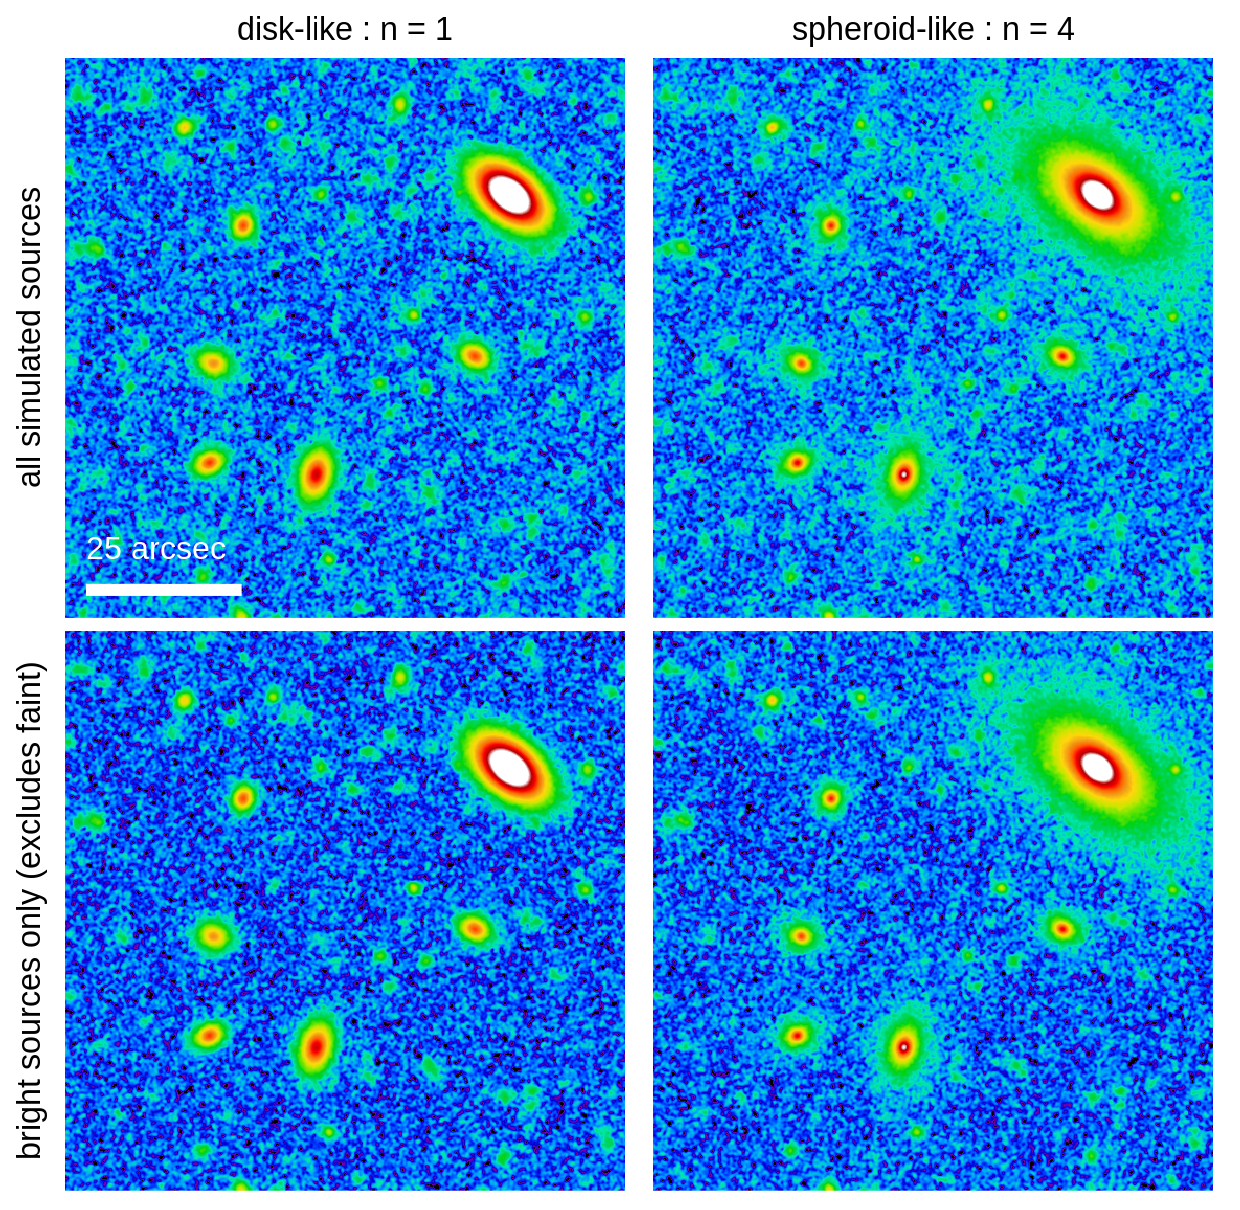
\includegraphics[width=0.9\textwidth]{{{fig/simstamp-zoom-8283-38}}}
    \caption{Low density simulated fields. As Figure \ref{fig:simstampfulllo}, but for a zoomed in region as represented by the inset scale. When zoomed in, the presence (top row) or otherwise (bottom row) of faint EBL sources and their impact on the apparent sky level is visibly evident.}
    \label{fig:simstampzoomlo}
\end{figure*}

Figure \ref{fig:simstampfullhi} shows the four simulated fields corresponding to the high density region. As with Figure \ref{fig:simstampfulllo}, the four panels represent the full and bright-only simulations for disk-like ($n=1$) and spheroid-like ($n=4$) sources as indicated by the marginal axis labels. Similar observations to those made for the low density region may be repeated here regarding the impact of faint sources and extended profiles on the apparent sky level pedestal. The effect of these biases is however significantly multiplied, owing to the increased number density of sources in this field. 

\begin{figure*}
    \centering
    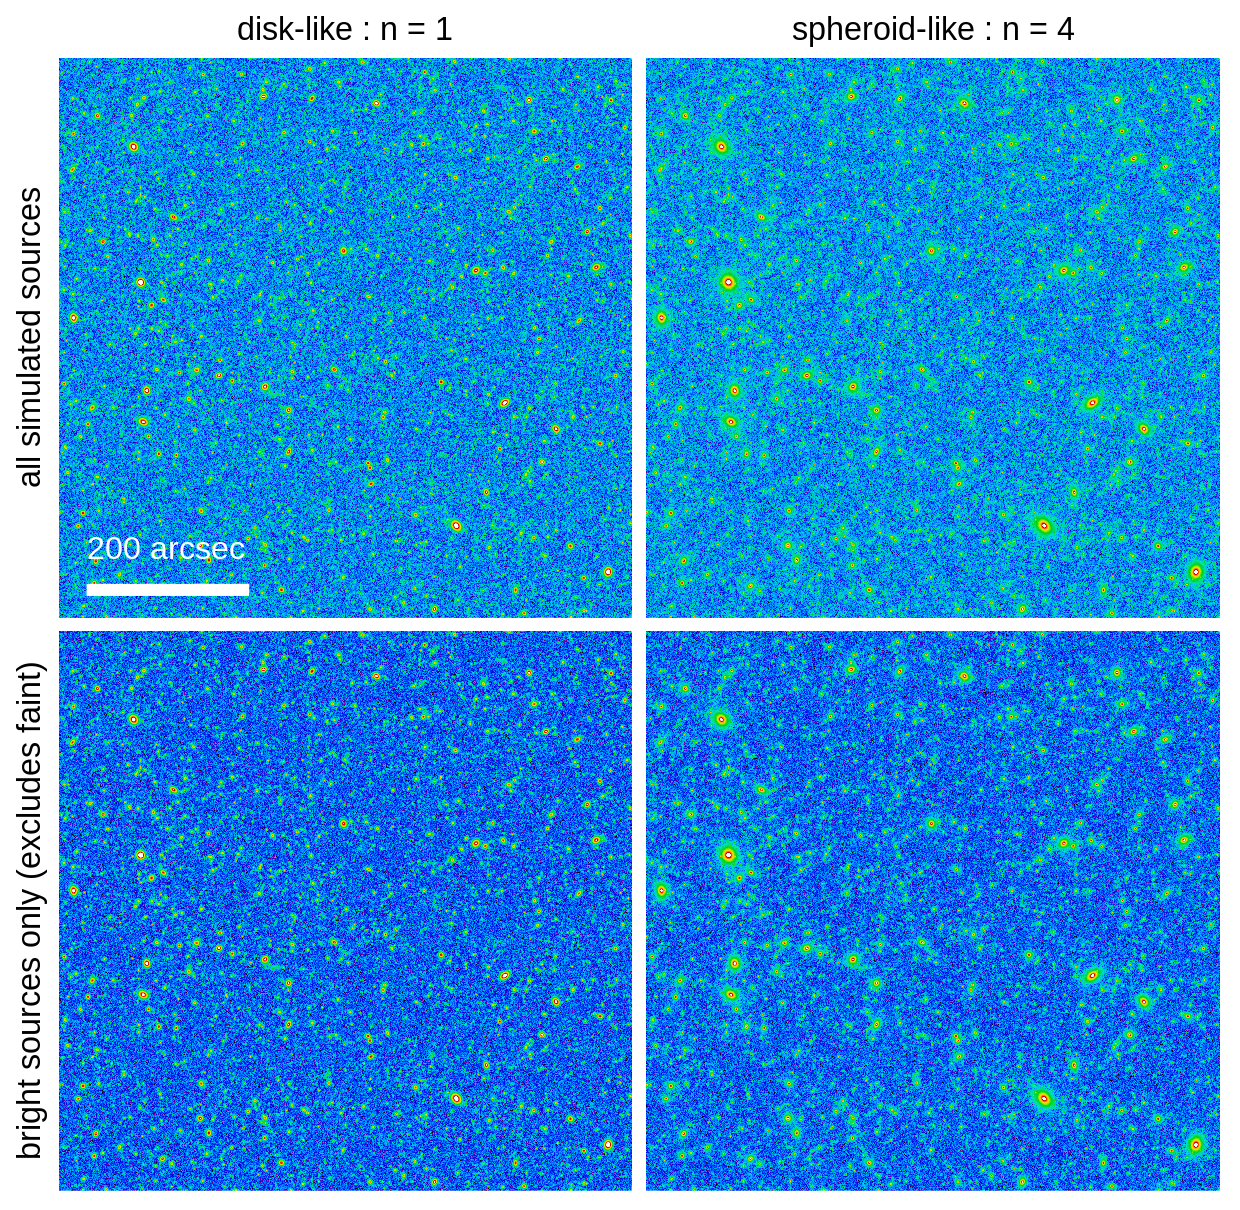
\includegraphics[width=0.9\textwidth]{{{fig/simstamp-full-9592-20}}}
    \caption{All four \GalSim simulated outputs for the high density `denhi' region. Top left: The full simulated high density field populated exclusively with exponential $n=1$ disk-like sources. Top right: The full simulated high density field populated exclusively with de Vaucouleurs $n=4$ spheroid-like sources. Bottom left: The bright end sub-population only (i.e., excluding faint missing sources), with each source described by an $n=1$ \Sersic profile. Bottom right: The bright end sub-populations only, with each source described by an $n=4$ \Sersic profile. The scale inset into the top left panel applies equivalently to all panels. All sources are PSF-convolved, and HSC-SSP PDR1 Poisson noise has been added. Images are arctan scaled. As with the low density region, the impact of source population and source profile type is visibly evident on the apparent background level.}
    \label{fig:simstampfullhi}
\end{figure*}

Figure \ref{fig:simstampzoomhi} shows four zoomed in views of the high density regions shown in Figure \ref{fig:simstampfullhi}, with the zoom factor represented by the inset scale. The zoom factor in this figure is identical to that used for Figure \ref{fig:simstampzoomlo}, i.e., each panel shown here shows the same solid angle on the sky as their equivalent panels in the low density regime. As noted above, the impact of faint sources is increasingly evident here. Not only do the numerous unresolved faint sources act to increase the global sky pedestal, but they also act to further enhance the wings of intermediate brightness galaxies. Such densely populated regions are becoming increasingly common in an era of low surface brightness astronomy, necessitating further study here. 

\begin{figure*}
    \centering
    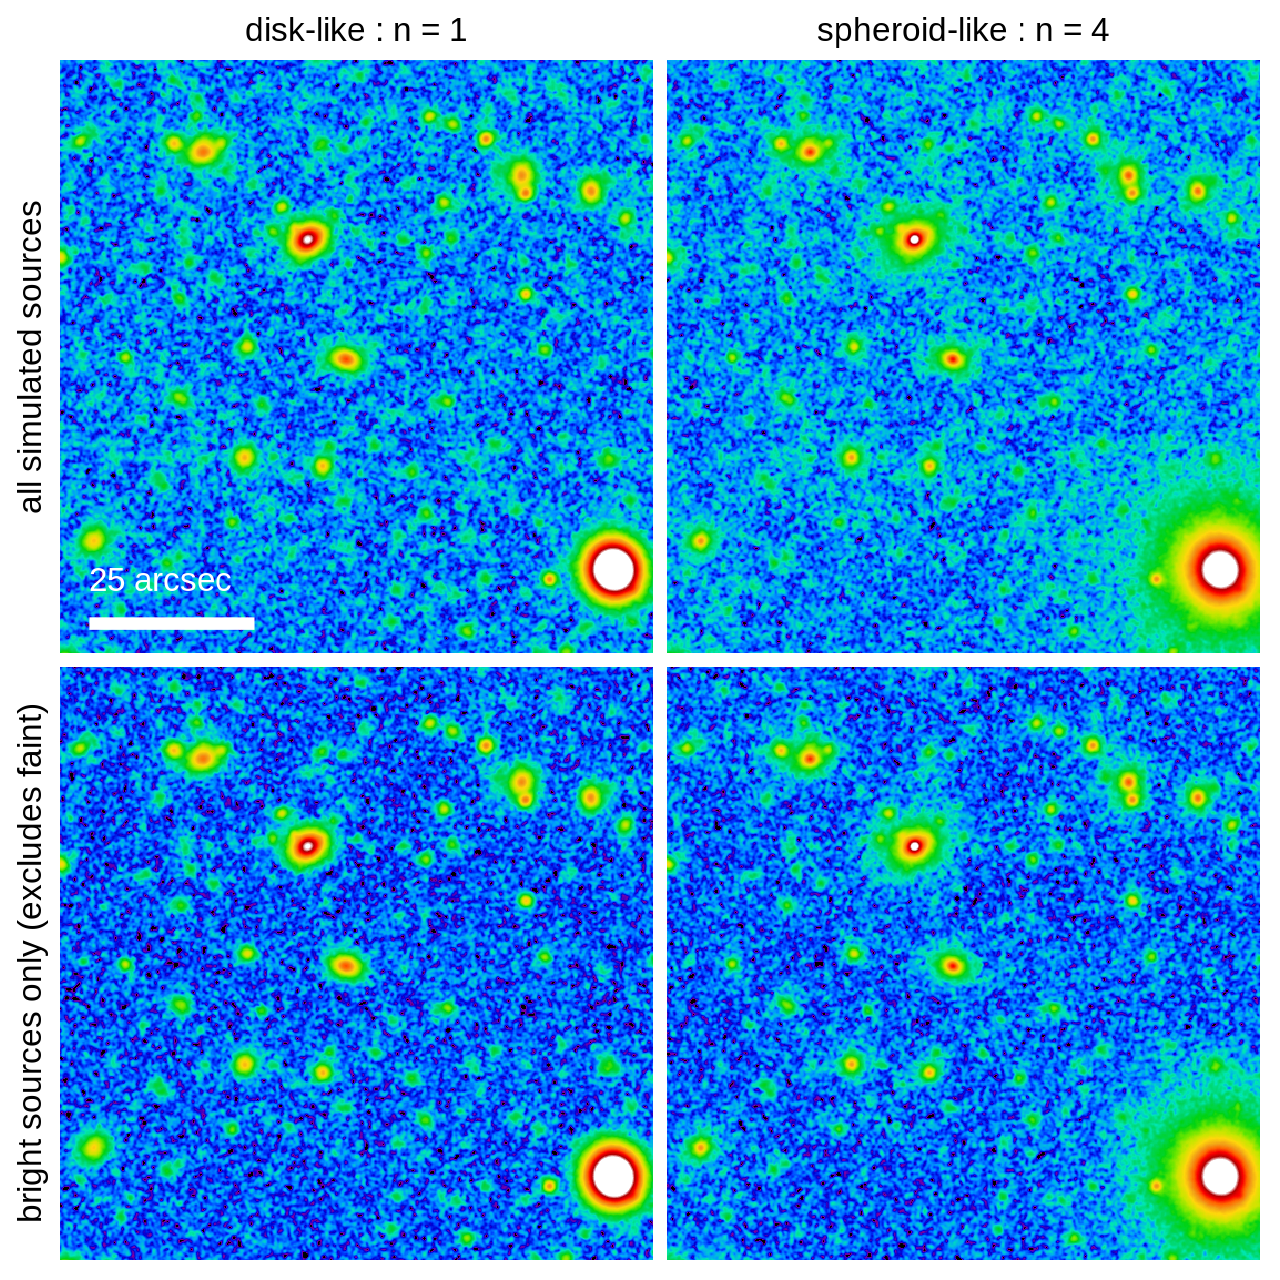
\includegraphics[width=0.9\textwidth]{{{fig/simstamp-zoom-9592-20}}}
    \caption{High density simulated fields. As Figure \ref{fig:simstampfullhi}, but for a zoomed in region as represented by the inset scale. As with the low density region, when zoomed in, the presence or otherwise of faint EBL sources and their impact on the apparent sky level is visibly evident.}
    \label{fig:simstampzoomhi}
\end{figure*}

The eight simulated fields summarised in Table \ref{tab:simtab} and shown in Figures \ref{fig:simstampfulllo} and \ref{fig:simstampfullhi} constitute our simulated dataset. These simulated images are background subtracted (i.e., Poisson noise oscillates about a level of zero counts) and populated with a range of extended PSF-convolved \Sersic profile objects. These simulated data are used for all subsequent analyses throughout the remainder of this study. 

\section{Source Extraction and Sky Estimation Techniques}
\label{sec:sextraction}

The sections above detail the construction of a comprehensive simulated HSC-SSP dataset consisting of objects spanning a range in source density, \Sersic index and EBL content. These data allow us to explore the robustness of various contemporary source extraction and sky estimation software routines. As introduced in Section \ref{sec:introduction}, we choose to employ the source extraction capabilities of three distinct software packages: \SExtractor, \textsc{Gnu Astronomy Utilities} (\Gnuastro), and the \RO \LSSTSPs \citep[hereafter, \LSSTPs]{Bosch2018,Bosch2019}. These three packages are chosen due to their significant usage within the astronomy community at large, and (notably in the case of the \LSSTPs) due to their anticipated importance in the reduction of future datasets. 

Each package is initially operated in a default mode configuration to provide a baseline comparison as to its capabilities. Such default configurations are often intended to maximally satisfy the general science goals of a broad and varied scientific user base. For the purposes of a specific science case however, it is often advisable to tweak these configuration parameters and modify the manner in which the software is used in order to best suit the requirements of the particular project. To address this, and in addition to our default runs, we further run each package in various configurations designed to optimally extract the background sky and associated source profiles. We begin this section below by presenting two novel techniques aimed at addressing these issues: dilated masking and modelled masking. Subsequent sections provide specific details on each distinct configuration setup explored within this study. 

\subsection{Magnitude Dependent Dilated Masking}
\label{sec:dilatedmasking}

As shown in \citet{Ji2018}, insufficient masking of bright extended sources can bias high any estimation of the background sky. Flux in the wings of such sources can easily leak out beyond a segmentation mask, causing a sky estimation algorithm to interpret these pixels as sky and erroneously attempt to subtract the associated flux. This effect is catastrophic for those interested in low surface brightness science, as it removes much of this LSB signal before scientific analyses can occur. Here we present the dilated masking method, a means by which such flux can be accurately accounted for in order to mitigate the effect of sky over-subtraction. 

Dilated masking enlarges the mask map associated with a particular object in such a way that those pixels containing flux from the wings of the source are brought underneath the mask. It is often beneficial to vary the amount of such dilated masking according to the magnitude of the underlying source, as in \citet{Ji2018}. Following experimentation with our input simulated dataset and software packages, we opt to expand the segmentation mask about a given detected object by a number of pixels $d$, where the extent of $d$ is related to its detected $r$-band magnitude $m_r$ as given by the following equation:
\begin{equation}
    \label{eq:dilmask}
    d = \lfloor10^{-0.2\left(m_r-25\right)}\rfloor + 5
\end{equation}
Relative to a bright source, progressively fainter objects will have their segmentation mask expanded by decreasing amounts, with the power law component of $d$ flattening out to zero pixels at magnitudes fainter than $m_r=25$ mag. Each masked region is additionally expanded by a fixed pixel amount of $5$ pixels. Segmentation masks are expanded using the \Gnuastro \textsc{arithmetic} software package. The implementation of this dilated masking prescription as applied to \SExtractor and \Gnuastro outputs is shown in Section \ref{sec:sextractordilated} and Section \ref{sec:gnuastrodilated}, respectively. 

\subsection{Modelled Masking}
\label{sec:modelledmasking}

An alternative approach towards identifying and correcting for flux leakage beyond the outer edge of a traditional isophotal segmented detection map is to attempt to model the surface brightness profile of the underlying source. The generation of a parametric model has many advantages, here allowing us to extrapolate such profiles out to large radii of our choosing and well into the noise. It is important to choose a viable model which is believed to sufficiently model the wings of the source, as choosing an incorrect or inaccurate model may produce inferior results than that of a default image processing procedure. 

We opt to model all detected sources brighter than $m_r=25$ mag with a PSF-convolved single \Sersic profile. Our rationale for limiting model fitting to bright sources alone is twofold. Firstly, if extended sources do act to negatively impact sky estimation routines, then it's the brightest of these sources that will have the largest per-object impact overall, with their broad wings overlapping a relatively larger number of secondary objects. Secondly, bright sources contain a larger number of pixels above the noise threshold, with their resultant best-fit models therefore of a higher certainty. The \citet{Sersic1963,Sersic1968} profile has long been successfully used to describe galaxy surface brightness profiles for a wide range of galaxy types \citep[e.g.,][]{Caon1993,Trujillo2004,Graham2005a,Hill2011,Simard2011,Kelvin2012,Kelvin2014a,Kelvin2014b}. Furthermore, our input simulated data has been generated using a range of PSF-convolved \Sersic profiles as described in Section \ref{sec:galsim}. Adopting PSF-convolved \Sersic models as our base descriptor of source surface brightness profiles therefore allows us to make a direct comparison of sky estimation software packages without needing to account for potential model inaccuracies.

All detected sources brighter than $m_r=25$ mag are fit using the \SExtractor software package. Whilst \SExtractor is well known for its source extraction capacity, its model fitting capabilities are less familiar. In concert with \PSFEx, \SExtractor is able to accurately and rapidly fit multiple model types to either all detected sources or a subset of detected sources\footnote{Subsets of the total detection catalogue are defined via source matching to $x$/$y$ coordinates and magnitude as provided by an \texttt{ASSOC} catalogue.}. Available model types include a PSF-like point source (\texttt{POINTSOURCE}), an exponential disk-like profile (\texttt{DISK}) and a generic \Sersic-like spheroid profile (\texttt{SPHEROID}). Specifying any of the associated profile fitting parameter names in the input parameter configuration catalogue will enable source fitting. A catalogue generated from an initial default run of \SExtractor and our previously described \PSFEx PSF model (see Section \ref{sec:psf}) are used as an input. We opt to fit our magnitude-limited subset sources using the \texttt{SPHEROID} \SExtractor model type\footnote{Complete \SExtractor catalogue parameters used for fitting in this instance are: \texttt{NUMBER}, \texttt{X\_IMAGE}, \texttt{Y\_IMAGE}, \texttt{FLUX\_SPHEROID}, \texttt{MAG\_SPHEROID}, \texttt{SPHEROID\_REFF\_IMAGE}, \texttt{SPHEROID\_ASPECT\_IMAGE}, \texttt{SPHEROID\_THETA\_IMAGE}, \texttt{SPHEROID\_SERSICN}, \texttt{CHI2\_MODEL}, \texttt{FLAGS\_MODEL} and \texttt{VECTOR\_ASSOC}. Further information may be found in \citet{Bertin1996} and associated documentation.}.

Once a catalogue of best fit \Sersic parameters is known, we use the \GalSim software package to construct model imaging. Whilst \SExtractor is also capable of outputting model imaging (using the \texttt{MODELS} check image type), these images were found to contain several edge artefacts that are not easily removed. We direct the interested reader to Section \ref{sec:postagestampsizes} for further details. For each source, the \SExtractor best fit output provides a starting $x$/$y$ coordinate location, total luminosity, half light radius, axis ratio, ellipticity and \Sersic index. In addition, \GalSim requires the user to specify the postage stamp box size within which the source is generated. As discussed in Section \ref{sec:postagestamps}, this postage stamp size should ideally encompass the entirety of our simulated image, mitigating potential edge effects. Due to computational expense however, some lower limit must be specified. We once again define a postage stamp size for each source such that the source profile reaches a surface brightness limit of $\mu_r=35\;\mathrm{mag\;arcsec}^{-2}$ at the extreme outer edge of the box, with a minimum box size of $11\times11$ pixels. This ensures that any profile boundary falls well within the noise, effectively eliminating its impact on our subsequent analyses. The resultant model image is finally subtracted from the initial science image, providing a new dataset upon which to estimate the sky with most of the bright source contaminant flux removed. The implementation of this modelled masking procedure as applied to \SExtractor and \Gnuastro outputs is shown in Section \ref{sec:sextractormodelled} and Section \ref{sec:gnuastromodelled}, respectively. 

\subsection{\SExtractor Configurations}
\label{sec:sextractor}

\subsubsection{Default \SExtractor Configuration}
\label{sec:sextractordefault}

The default setup of \SExtractor used at this stage of processing is identical to that outlined in Section \ref{sec:sample}, with the convolution kernel, stellar classification neural network file and configuration file preserved exactly. The threshold for source detection is maintained at $1.5\sigma$ of the background estimate. Having excluded detected sources, background sky in \SExtractor is estimated across the image within a default of $64\times64$ pixel \texttt{BACK\_SIZE} mesh elements. A bicubic-spline interpolation is subsequently applied to all mesh elements to produce a background map, allowing for the exclusion of erroneous mesh values if necessary. In addition to the output catalogue parameters defined in Section \ref{sec:sample}, we also opt to output \texttt{ISOAREA\_IMAGE}, providing data on the total area above the analysis threshold for each detected object. The \SExtractor package is run upon each simulated image, producing an output catalogue and check images for the segmentation map (\texttt{SEGMENTATION}), background pedestal map (\texttt{BACKGROUND}) and background RMS map (\texttt{BACKGROUND\_RMS}). Further information on the default operation of \SExtractor may be found in \citet{Bertin1996}.

\subsubsection{Modified \SExtractor Configuration}
\label{sec:sextractormodified}

The \SExtractor package is often modified in order to better tailor its outputs to the specific scientific needs of ones dataset. A sky estimation and source detection setup which may prove optimal for the characterisation of point-like sources is often wholly inadequate for the purposes of extended source analysis. Modifications are also often made to address common complaints with the default outputs of \SExtractor \citep[see, e.g.,][]{Haussler2007, Haussler2013, Simard2011, Barden2012, Kelvin2012, Hiemer2014}. Principal amongst these are issues surrounding the derived sky level, an inadequate smoothing kernel, and inaccurate source segmentation. There is a long and inglorious history to such segmentation failures in top-down auto-detect algorithms. For a number of years in the field of Source Extraction \citep[see e.g. \textsc{FOCAS},][]{Jarvis1981} such segmentation failures have often been encountered when using low threshold runs of \SExtractor, largely in situations where there is a triangle of objects that fail proper segmentation and photometry. This geometry can create a situation where there is no 1-D saddle point in the surface brightness.

We adopt five key \SExtractor configuration modifications to address these issues. First, we increase the background mesh element size (\texttt{BACK\_SIZE}) to $128\times128$ pixels (from a default of $64\times64$ pixels). An increase of this type reduces the risk that any individual mesh element becomes severely compromised by source flux from a single bright object or cluster of bright objects. Second, we also increase the background mesh filter size (\texttt{BACK\_FILTERSIZE}) to $5$ (from a default of $3$). This filtering size determines the mesh super-pixel area over which mesh elements are filtered to detect and eliminate background estimate outliers. A larger filter size increases the identification of outliers, providing a more coherent global sky estimate. Third, to assist with initial source detection, we reduce the detection and analysis thresholds (\texttt{DETECT\_THRESH} and \texttt{ANALYSIS\_THRESH}) to $0.5\sigma$ (from a default of $1.5\sigma$), and fourth, we replace the default smoothing kernel with a Gaussian of FWHM $\Gamma=2$ pixels. A larger smoothing kernel reduces the impact of contaminant noise spikes present within the background and allows for a lower overall source detection threshold. Finally, we reduce the minimum segmentation contrast parameter (\texttt{DEBLEND\_MINCONT}) to $0.00005$ (from a default of $0.005$). As highlighted in the draft \SExtractor manual~\citep{SExtractorUsersManual}, reducing this value increases the chance that faint local peaks will be included as separate objects. Whilst this does not directly impact the final sky estimate, it does produce superior segmentation results within contiguous regions falling above the detection threshold, necessarily improving source extraction catalogue data. 

\subsubsection{\SExtractor with Dilated Masks}
\label{sec:sextractordilated}

It is not natively possible to apply the dilated masking process outlined in Section \ref{sec:dilatedmasking} within \SExtractor itself. Implementation of this procedure therefore requires modifying the data that is fed into \SExtractor. First, dilated masks are produced using a default \SExtractor run. Using the input science image, each masked pixel is set equal to \texttt{NaN}. Such pixels will not be used by \SExtractor to construct a background map. Finally, this new manually masked image is processed using the same default \SExtractor setup as previously used. 

An example of the dilated masking routine as applied to the simulated data initially presented in Figure \ref{fig:simstampzoomlo} and subsequently processed by \SExtractor is shown in Figure \ref{fig:dilmask_sex}. The upper left panel shows our previously presented zoomed in $n=4$ low density simulated field (denlo4a), arctan scaled and smoothed with a Gaussian kernel of $\Gamma=3\;\mathrm{pix}$. The lower left panel shows the segmentation map for this region as produced using a default \SExtractor run. Each segmented region is colour coded according to the total detected $r$-band magnitude of the underlying source, as represented by the inset colour bar. The upper central panel shows the default segmentation map overlaid upon the initial image, whilst the lower central panel shows our magnitude dependent dilated masks overlaid upon the initial image. Finally, the upper right and lower right panels show the output background sky maps as determined using the original default segmentation map and the new dilated mask map, respectively. 

\begin{figure*}
    \centering
    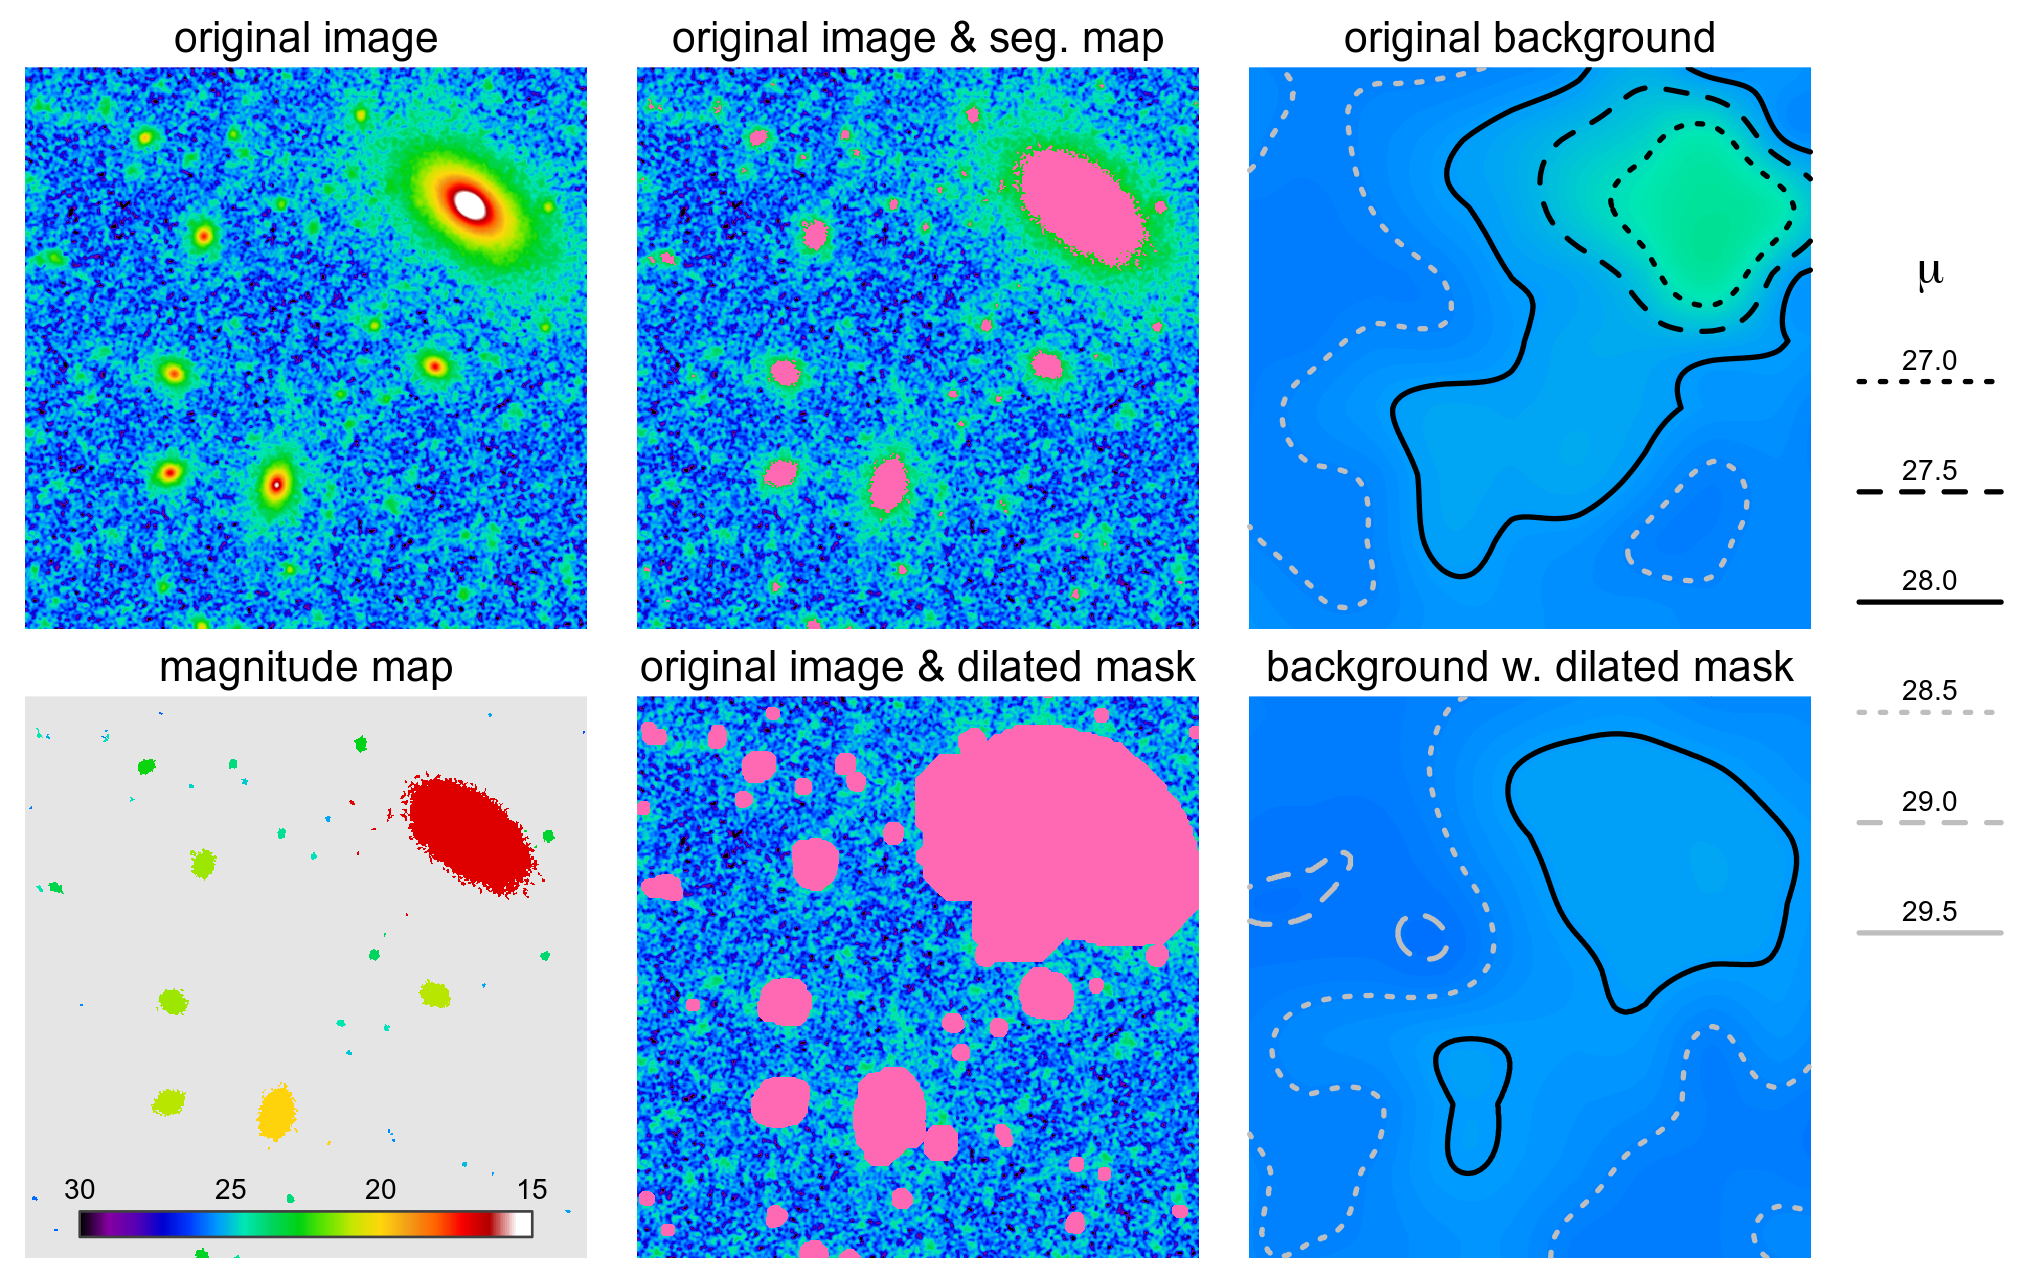
\includegraphics[width=1.0\textwidth]{{{fig/dilmask_sex}}}
    \caption{An example of dilated masking as applied to a zoomed in $n=4$ low density simulated field (denlo4a) and processed using the \SExtractor software package. Top left: the original simulated dataset, corresponding to the same zoomed in region previously shown in Figure \ref{fig:simstampzoomlo}. Bottom left: the segmentation map for this region as given by a default run of \SExtractor. Each segmented region is colour coded according to its underlying detected source magnitude, as shown by the inset colour bar. Top centre: the original segmentation map overlaid upon the original image. A significant amount of flux can be seen leaking out beyond the default segmented regions, thereby contaminating any estimate of the sky. Bottom centre: the new dilated mask overlaid upon the original image. The extent of mask dilation is magnitude dependent, as given by Equation \ref{eq:dilmask}. These larger dilated masks are superior at masking signal around the wings of bright sources. Top right: the original estimate of the background sky as found when using default segmentation masks. A notable contamination due to the bright extended source within this field is evident. Bottom right: the new estimate of the background sky as found when using the dilated masks shown here. Much of the aforementioned background sky contamination is improved, resulting in a flatter and more accurate sky estimate. Background map line contours are equivalent to surface brightness limits in units of $\mathrm{mag\;arcsec}^{-2}$ shown in the outlying legend. Images are arctan scaled, with noisy imaging smoothed by a Gaussian kernel of $\Gamma=3\;\mathrm{pix}$.}
    \label{fig:dilmask_sex}
\end{figure*}

As shown, a significant amount of flux is evidently leaking from the outskirts of the default segmentation map. Further, the amount of flux leakage appears linked to the brightness of the underlying source, with the majority of the contamination in this particular field linked to the large bright source in the upper right corner. Application of magnitude-dependent dilated masks significantly reduces the amount of contaminant flux present in the remaining background pixels, markedly improving the resultant background sky estimate. 

\subsubsection{\SExtractor with Modelled Masks}
\label{sec:sextractormodelled}

Input data must first be modified in order to facilitate the use of modelled masks with \SExtractor. We begin by subtracting our multi-\Sersic model image from our initial dataset. This produces a residual image for all sources not included within the model (i.e., typically sources fainter than our $m_r=25$ mag fitting limit). The removal of bright source wings allows for a more accurate estimate of the sky in these regions, whilst simultaneously markedly improving source characterisation for small faint sources previously hidden beneath the skirts of their bright neighbours. The centres of bright astrophysical sources are notoriously difficult to fit, with even a slight model inaccuracy resulting in a pixel value offset of many multiples of the background RMS. To prevent such regions having any impact upon our sky estimation routine, we manually apply the original default \SExtractor segmentation mask to our residual image, setting masked pixels equal to \texttt{NaN}. Such pixels will be ignored by \SExtractor when generating sky estimates and whilst performing source extraction. 

An example of the modelled masking routine as applied to our simulated data is shown in Figure \ref{fig:modmask_sex}. The top left panel shows our original simulated image (see Figure \ref{fig:simstampzoomlo}). The bottom left panel shows the same simulated image overlaid with the default \SExtractor segmentation mask map. The top centre panel shows the fitted PSF-convolved multi-\Sersic model generated for this region. All detected sources brighter than $m_r=25$ mag are fit. The bottom centre panel shows the residual image generated once the fitted model is removed from the original image. The original \SExtractor segmentation map is overlaid. As can be seen, much of the contaminant flux leaking out from the segmented regions has been successfully accounted for. The top right panel shows the initial estimate of the background sky using the default \SExtractor setup, whilst the bottom right panel shows the background sky resulting from a modelling masked processed image. The difference between the two is stark, with multiple orders of magnitude difference in the resultant background sky estimate. Notably, the impact of the singular bright source has been almost completely accounted for, leaving behind a much flatter sky estimate in its place. 

\begin{figure*}
    \centering
    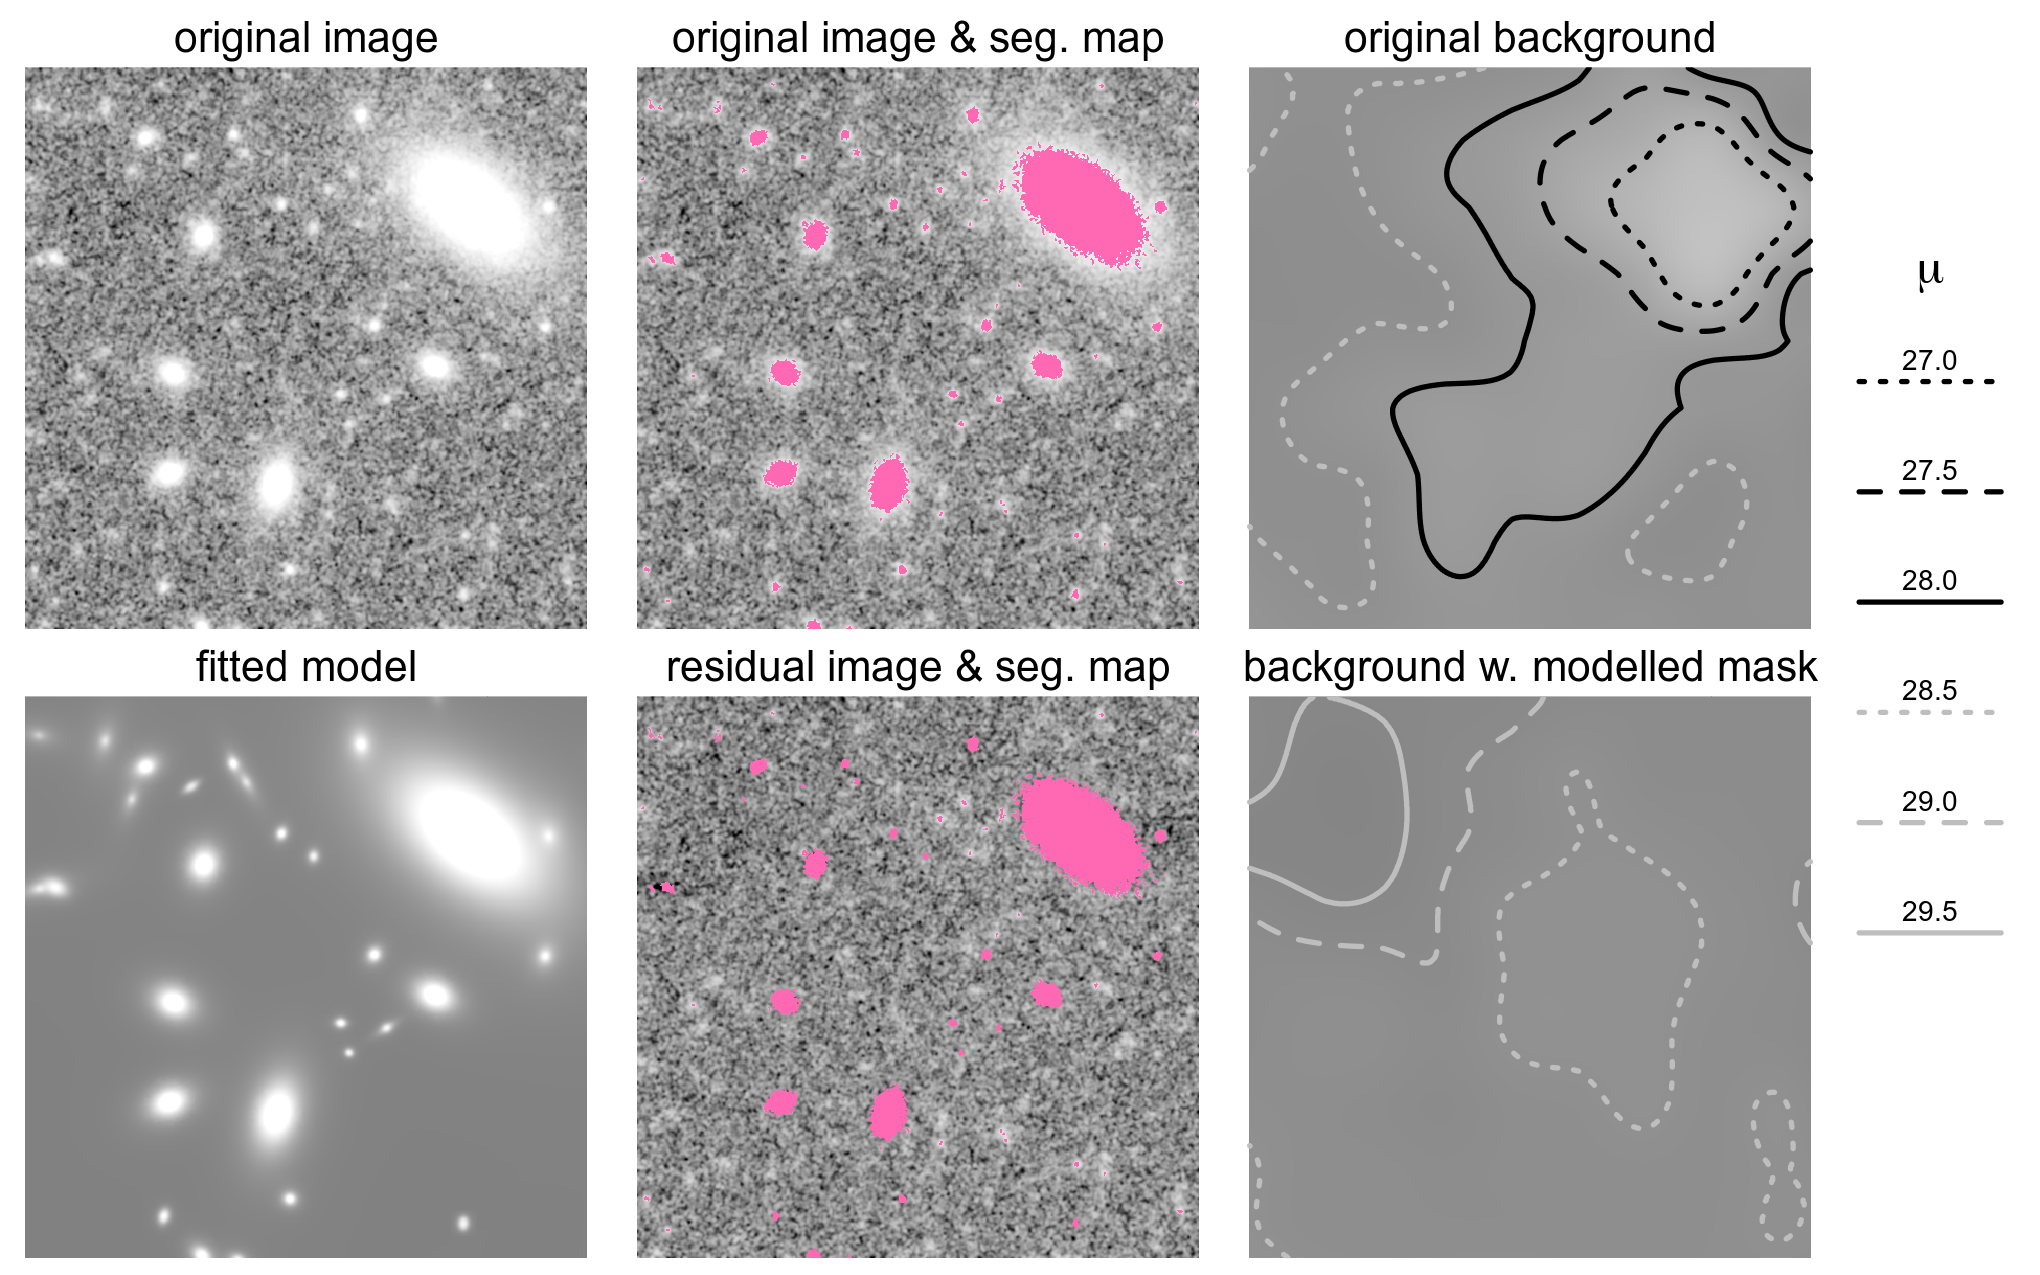
\includegraphics[width=1.0\textwidth]{{{fig/modmask_sex}}}
    \caption{An example of modelled masking as applied to a zoomed in $n=4$ low density simulated field (denlo4a) and processed using the \SExtractor software package. Top left: the original simulated dataset (see Figure \ref{fig:simstampzoomlo}). Bottom left: the original image with the default \SExtractor segmentation map overlaid. Top centre: the successfully fitted single \Sersic models based upon detected sources brighter than $m_r=25$ mag. Bottom centre: the residual image generated after the fitted model is removed from the original image, overlaid with the default \SExtractor segmentation map. Note how much of the prior contaminant flux observed leaking from beyond the edge of the segmented regions has been removed. Top right: the original estimate of the background sky as produced using a default \SExtractor run. The dominant source in this field has severely compromised the sky estimate in this region. Bottom right: the new estimate of the background sky generated when using modelled masks. The sky estimate is significantly improved, no longer exhibiting strong source-correlated sky biases. Background map line contours are equivalent to surface brightness limits in units of $\mathrm{mag\;arcsec}^{-2}$ shown in the outlying legend. Images are arctan scaled, with noisy imaging smoothed by a Gaussian kernel of $\Gamma=3\;\mathrm{pix}$.}
    \label{fig:modmask_sex}
\end{figure*}

\subsection{\Gnuastro Configurations}
\label{sec:gnuastro}

\subsubsection{Default \Gnuastro Configuration}
\label{sec:gnuastrodefault}

The \Gnuastro software suite is highly modularised, necessitating the use of several sub-packages to fully process any given dataset. Each simulated image is initially processed by \NoiseChisel, the \Gnuastro source detection and sky estimation package designed to optimally extract sources with extended profiles embedded within noisy data. In brief, pixel data is first convolved with a Gaussian smoothing kernel and thresholded at some pixel value quantile (e.g., the $30^{\mathrm{th}}$ percentile) within mesh elements of default size $30\times30$ pixels, splitting the image into regions of noise and regions of signal. A series of erosions and dilations are subsequently performed on the regions of noise (i.e., the noise is `chiselled') and false detections are removed. Any remaining regions of signal undergo further pixel dilation. Once regions believed to contain true signal flux have been determined, the \Segment package splits these regions into distinct sources, performing clump-based segmentation where required. Finally, the \MakeCatalog package is used to convert processed pixel data into an output source catalogue\footnote{Output \Gnuastro \MakeCatalog columns are: \texttt{ids}, \texttt{x}, \texttt{y}, \texttt{brightness}, \texttt{magnitude}, \texttt{semimajor}, \texttt{semiminor}, \texttt{geosemimajor}, \texttt{geosemiminor}, \texttt{sn}, \texttt{axisratio}, \texttt{positionangle}, \texttt{sky}, \texttt{std}, \texttt{area} and \texttt{upperlimit}. A full description for each column output may be found in \citet{Akhlaghi2015}}. Further information on the operation of all \Gnuastro packages may be found in \citet{Akhlaghi2015}.

\subsubsection{Modified \Gnuastro Configuration}
\label{sec:gnuastromodified}

As with \SExtractor, a number of typical modifications may also be made to the operation of \Gnuastro in order to improve or tailor its output results. Owing to the modularised nature of \Gnuastro, some modifications are made to all utilised sub-packages, whilst others are specific to individual sub-packages. We detail all modifications here. 

First, we opt to modify the default mesh size of $30\times30$ pixels used during initial background estimation using the \texttt{tilesize} argument. The tile size determines the mesh size within which initial background thresholding occurs. In the presence of large sky gradients or large contaminant sources, an overly-large tile size may lead to a significant amount of data either being discarded or erroneously classified. We therefore opt to decrease the tile size to $15\times15$ pixels, helping to minimise these effects. The tile size parameter is globally provided to \NoiseChisel, \Segment and \MakeCatalog.

Second, we opt to reduce the threshold down to which \NoiseChisel detection maps are expanded using the \texttt{detgrowquant} parameter. The detection growth quantile (default $0.9$) determines down to what quantile `true' detections are expanded out into the noise. This growth mechanism is superior to traditional dilation, as it allows the user to follow the shape of the profile out into the noise. Such an effect is crucial in accurately capturing more of the diffuse low surface brightness light typically located around the wings of bright extended sources. However, setting this value too low leaves open the possibility that spurious noise signals will end up being drawn into the final resultant detection maps. We opt to lower the detection growth quantile parameter to $0.7$, somewhat expanding our detection footprints relative to the defaults to capture more of the low surface brightness flux, yet sufficiently high to remain robust against noise contamination. 

We note that a number of additional parameters were explored and rejected here, owing to their failure to significantly improve sky estimation or source extraction results. These include modifications in: the smoothing kernel, the maximum mean and median quantile difference per tile, the quantile threshold on the convolved image, the quantile threshold determining which pixels are excluded from erosion, the selection of sky tiles and quantile of the signal-to-noise ratio distribution of clumps in undetected regions. 

\subsubsection{\Gnuastro with Dilated Masks}
\label{sec:gnuastrodilated}
Figure \ref{fig:dilmask_gnuastro} shows the dilated masking routine as applied to simulated data which has been processed by \Gnuastro. Each panel is equivalent to the panels previously shown in Figure \ref{fig:dilmask_sex}, excepting that the segmentation maps and subsequent dilated masks are based upon \Gnuastro source extraction processing. As previously seen, the effect of the dilated masking procedure is to significantly reduce the impact of flux leakage upon the final background sky estimate. We note however that the original segmented region produced by \Gnuastro covers a much larger fraction of the original image than \SExtractor. Consequently, the original default background sky produced by \Gnuastro is markedly less impacted by the bright source in this region than the default outputs from a \SExtractor run. This will be further discussed in Section \ref{sec:results}.

\begin{figure*}
    \centering
    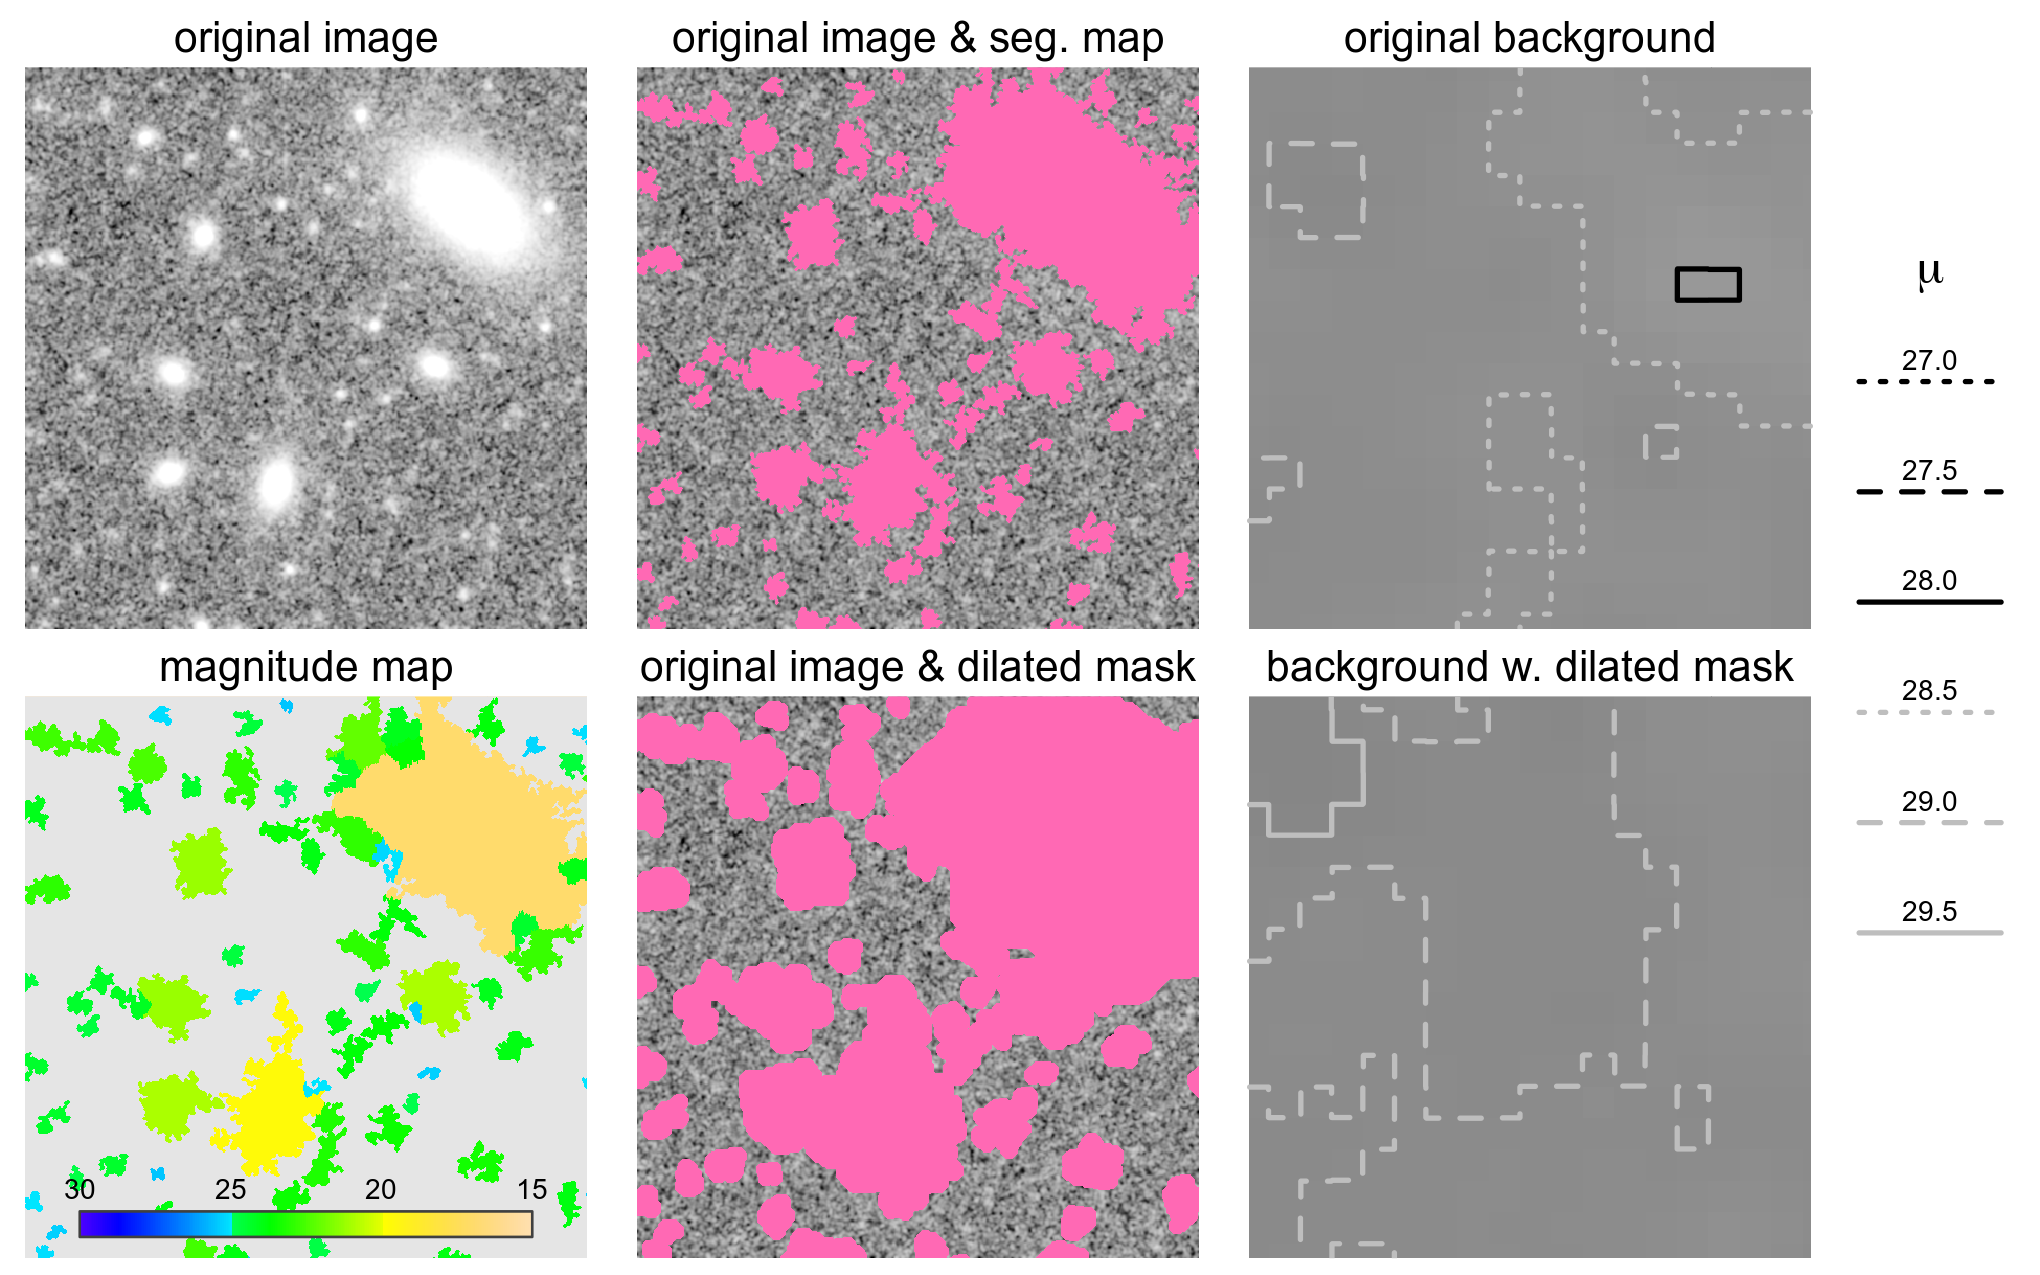
\includegraphics[width=1.0\textwidth]{{{fig/dilmask_gnuastro}}}
    \caption{An example of dilated masking as applied to a zoomed in $n=4$ low density simulated field (denlo4a) and processed using the \Gnuastro software package. Panels are defined as in Figure \ref{fig:dilmask_sex}, with the dilated masking procedure applied to simulated data processed instead by \Gnuastro. Background map line contours are equivalent to surface brightness limits in units of $\mathrm{mag\;arcsec}^{-2}$ shown in the outlying legend. Images are arctan scaled, with noisy imaging smoothed by a Gaussian kernel of $\Gamma=3\;\mathrm{pix}$. The effect of performing sky estimation on a dilated mask image is evident, removing the contaminant impact of bright sources and pushing recovered sky maps down to very faint estimates.}
    \label{fig:dilmask_gnuastro}
\end{figure*}

\subsubsection{\Gnuastro with Modelled Masks}
\label{sec:gnuastromodelled}

Figure~\ref{fig:modmask_gnuastro} shows the effect of modelled masking as applied to simulated data which has been processed by \Gnuastro. Each panel is equivalent to the panels previously shown in Figure~\ref{fig:modmask_sex}, except that the segmentation maps and derivative modelled mask data are based upon \Gnuastro source extraction processing. The impact of modelled masks appears to somewhat aid the background estimator in producing an unbiased background map. Whilst the initial segmentation map is already reasonably extensive as previously noted, the model masking procedure further removes any remnant contamination from the wings of the bright sources shown in this figure. A more complete discussion of the impact of modelled masking here will be further discussed in Section~\ref{sec:results}.

\begin{figure*}
    \centering
    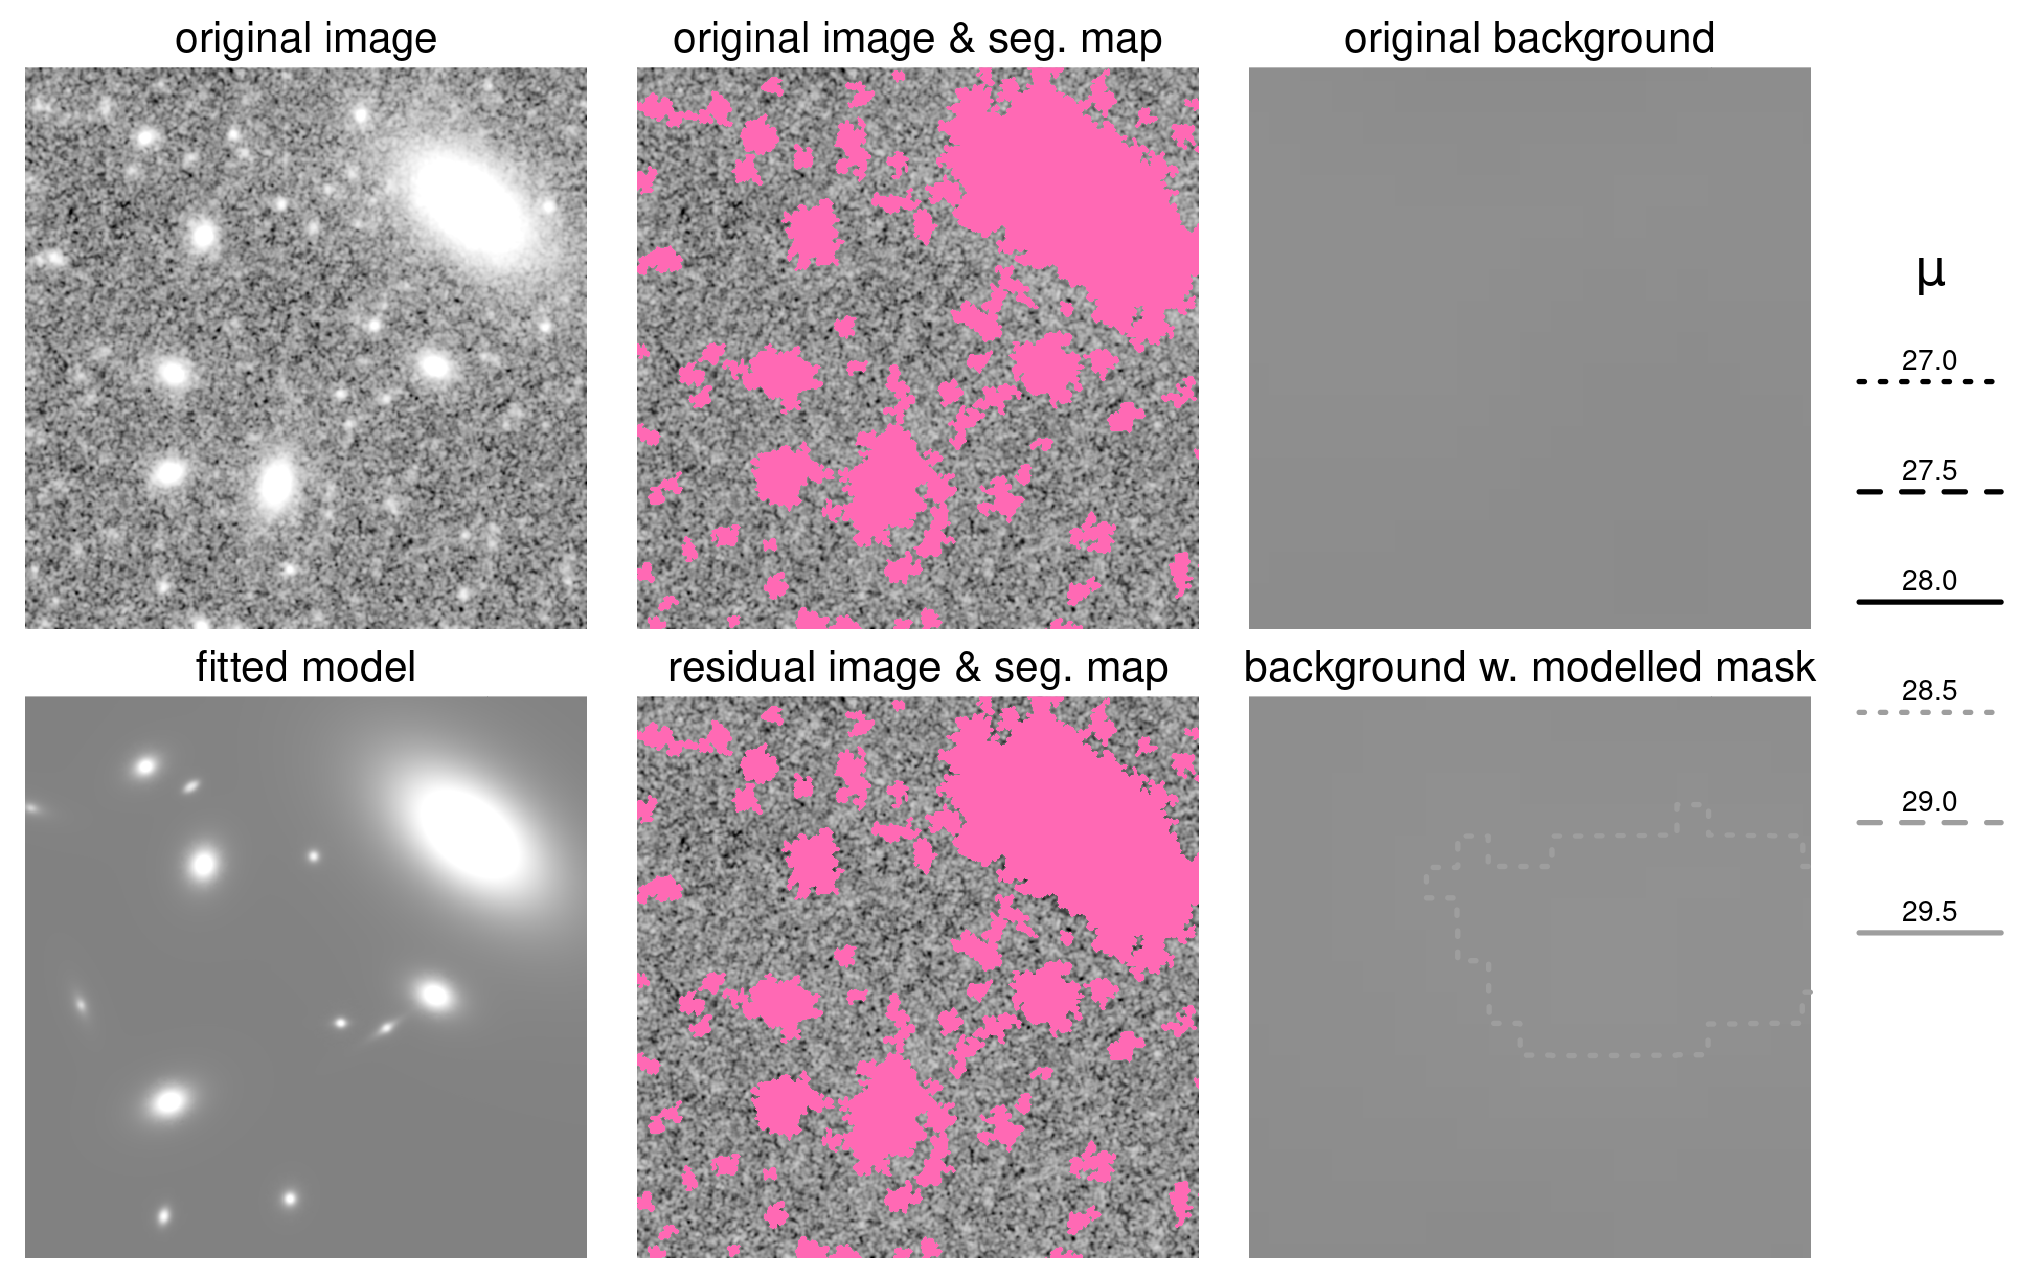
\includegraphics[width=1.0\textwidth]{{{fig/modmask_gnuastro}}}
    \caption{An example of modelled masking as applied to a zoomed in $n=4$ low density simulated field (denlo4a) and processed using the \Gnuastro software package. Panels are defined as in Figure \ref{fig:modmask_sex}, with the modelled masking procedure applied to simulated data processed instead by \Gnuastro. Background map line contours are equivalent to surface brightness limits in units of $\mathrm{mag\;arcsec}^{-2}$ shown in the outlying legend. Images are arctan scaled, with noisy imaging smoothed by a Gaussian kernel of $\Gamma=3\;\mathrm{pix}$. As can be seen here, the application of modelled masks acts to noticeably reduce contamination from previously unmasked contaminant flux around the wings of bright sources, producing an improved and flatter background map.}
    \label{fig:modmask_gnuastro}
\end{figure*}

\subsection{Configurations of the \LSSTPs}
\label{sec:dmstack}

The \RO \LSSTPs has been designed to optimally process HSC and LSST type imaging, performing a number of complex image processing routines to ultimately produce high fidelity output catalogue and imaging data. This software stack has been working with HSC data for a number of years, making it an ideal candidate for use with the simulated HSC-type imaging produced for this study. We process our simulated data with two realisations of the \LSSTPs, version 19.0.0. First, these data are analysed with a specific configuration of the \LSSTPs designed to mimic an earlier state of the code base utilising a sixth-order polynomial fit to describe the background model. The code base at this time is largely equivalent to that used to initially produce HSC-SSP PDR1 data, and serves as a useful baseline. Second, we process our simulated datasets with an updated configuration of the \LSSTPs designed to mimic the current state of the code base at the time of writing, employing a more local 128-pixel spline to describe the background model. Both such configurations are further discussed in the sections below. Further details may be found in \citet{Bosch2018} and \citet{Bosch2019}.

\subsubsection{\LSSTPs Sixth Degree Polynomial Configuration (\DMA)}
\label{sec:dmstack2018}

The first configuration of the \LSSTPs explored here is one which generates a background map using a sixth degree polynomial fit to detected background pixels (hereafter referred to as `\DMA', for brevity). Simulated image data is initially convolved with a smoothing kernel, and contiguous regions above some threshold level are identified. In a standard run of the \LSSTPs (i.e., using true astrophysical data), high signal-to-noise stars are identified on the stellar locus using a placeholder Gaussian PSF to perform a first detection pass. These bright stars are then used to model the spatially varying PSF over the image using \PSFEx. A circular Gaussian whose RMS width is matched to the PSF is used as a detection kernel for performance reasons. However, as the simulated imaging constructed for use within this study contains no point sources (see Section \ref{sec:galsim}) we do not follow this procedure here. Instead, we construct a circular Gaussian whose RMS width is matched to the PSF described in section \ref{sec:psf}. This circularised Gaussian is subsequently used as our primary detection kernel. 

Background estimation within the \LSSTPs is handled by the \textsc{SubtractBackgroundTask} method. The astrophysical background contains contributions from several sources: the night sky, optical ghosts and scattered light in the telescope, and undetected sources that make up the EBL amongst them. A parametric model based upon the sum total of these contributions to the background is constructed and subsequently subtracted out at the image level. The process consists of two high-level steps. First, the image is subdivided into $128\times128$ pixel bins, or \textit{super pixels}. Pixels which constitute each super pixel and do not correspond to any detected object are used to calculate the mean, variance, and pixel averaged centre of its host super pixel. Second, a 6th order two-dimensional Chebyshev polynomial model is fit to the mean values of the image, using the average pixel centres of each super pixel. Each bin is inverse weighted by its variance such that noisy super pixels with relatively few unmasked regions do not overly bias the fit. 

\subsubsection{\LSSTPs 128-Pixel Spline Configuration (\DMB)}
\label{sec:dmstack2020}

The second configuration of the \LSSTPs explored here generates a background map using a $128$ pixel spline fit to all identified background pixels (hereafter referred to as `\DMB', for brevity). This configuration makes use of an alternate detection algorithm which is better suited towards detecting EBL galaxies and LSB flux. In the \LSSTPs \DMA configurations, the detection threshold is fixed at $5\sigma$ across the whole field, where $\sigma^2$ is the variance. However, the variance estimation may be incorrect after convolution owing to the fact that convolution correlates the noise. This leads to an under-performance in the detection algorithm, where recognisable-by-eye sources are not detected \citep[see][Figure 5]{Aihara2019}. To mitigate these effects, we run the high level process \textsc{DetectCoaddSourcesTask} in the \DMB configuration, which adopts the \textsc{DynamicDetectionTask} in the \LSSTPs in lieu of the default detection package used in the \DMA configuration. In the \textsc{DynamicDetectionTask} mock PSFs are injected into the image in regions of mostly empty sky, ensuring that detected objects are avoided. The ratio between the standard deviation of PSF fluxes of the points to the variance over the effective area of the PSF provides a correction factor to the detection threshold, dynamically adjusting it across the image. 

To implement this optimised setup, image data is initially processed in a manner consistent with that described above. Sources are detected, masked, and the remaining simulated imaging is subdivided into $128\times128$ super pixel bins. A $3\sigma$ clipped mean is computed among all non-masked pixels inside each super-pixel, and a two-dimensional 6th order bilinear spline is fit to these super pixel means. This creates a full resolution image of the sky background model. At the time of writing, the procedure outlined above is consistent to what is being done for the HSC Internal Data Release S19A, mirroring how coadded images are presently being processed by the \LSSTPs. 

\section{Results}
\label{sec:results}

Following the procedures described above, we have generated background sky estimates and source detection results for a number of simulated datasets. A total of eight HSC-SSP PDR1 fields have been simulated in three binary flavours: fields with faint EBL sources either included or excluded; fields of either a high or a low source density; and fields populated exclusively with either exponential ($n=1$) or de Vaucouleurs ($n=4$) radial profile source types. These data have been processed in $10$ software configuration modes: four configurations of the \SExtractor software package, four configurations of the \Gnuastro software suite, and two configurations of the \LSSTPs. 

Our full sky estimation results are shown in Table \ref{tab:results}. Each cell in this table shows the estimated mean and standard deviation (in units of $e^{-}/\textrm{pixel}$) of the recovered background sky model for each flavour of simulated data (per column) and software configuration mode (per row). Counts per pixel on output background statistics are converted to $e^{-}/\textrm{pixel}$ using the equivalent gains presented in Section \ref{sec:gainskylevel}. As a reminder, all simulated datasets are background subtracted (the input sky was set to zero), so recovered sky values closer to zero are more desirable here. Common trends become apparent, and are explored below. We begin by discussing global sky estimation trends visible between all flavours of binary data type regardless of any specific software configuration in Section \ref{sec:flavour}. Following this, we then compare each software configuration mode against one another in the context of output sky levels in Section \ref{sec:mode} to discover desirable sky estimation and source extraction techniques. Finally, we move beyond analysis of the output sky levels and sky maps to take a closer look at the fidelity of output source catalogues in Section \ref{sec:fidelity}.

\begin{table*}
    \setlength{\tabcolsep}{5pt}
    \begin{tabular}{ l | r | r | r | r | r | r | r | r }
    \multicolumn{1}{r}{source population :} & \multicolumn{4}{c}{including all sources} & \multicolumn{4}{c}{excluding faint sources}\\
    \multicolumn{1}{r}{source density :} & \multicolumn{2}{c}{low density} & \multicolumn{2}{c}{high density} & \multicolumn{2}{c}{low density} & \multicolumn{2}{c}{high density}\\
    \multicolumn{1}{r}{source type :} & \multicolumn{1}{c}{1} & \multicolumn{1}{c}{4} & \multicolumn{1}{c}{1} & \multicolumn{1}{c}{4} & \multicolumn{1}{c}{1} & \multicolumn{1}{c}{4} & \multicolumn{1}{c}{1} & \multicolumn{1}{c}{4}\\
    % begin copy-paste
    \multicolumn{1}{r}{label :} & \multicolumn{1}{c}{(denlo1a)} & \multicolumn{1}{c}{(denlo4a)} & \multicolumn{1}{c}{(denhi1a)} & \multicolumn{1}{c}{(denhi4a)} & \multicolumn{1}{c}{(denlo1b)} & \multicolumn{1}{c}{(denlo4b)} & \multicolumn{1}{c}{(denhi1b)} & \multicolumn{1}{c}{(denhi4b)}\\
    \hline
    \SExtractor & & & & & & & & \\
    \hspace{25pt}default & $3.8\pm0.9$ & $4.6\pm1.6$ & $5.7\pm0.9$ & $7.0\pm1.9$ & $1.0\pm0.8$ & $1.6\pm1.5$ & $1.7\pm0.9$ & $2.7\pm1.9$\\
    \hspace{25pt}modified & $3.8\pm0.5$ & $4.5\pm0.6$ & $5.8\pm0.4$ & $6.9\pm0.7$ & $1.0\pm0.3$ & $1.5\pm0.5$ & $1.7\pm0.4$ & $2.7\pm0.7$\\
    \hspace{25pt}w. dilated masks & $2.9\pm0.6$ & $3.8\pm0.9$ & $4.4\pm0.6$ & $5.8\pm0.9$ & $0.2\pm0.5$ & $0.9\pm0.8$ & $0.5\pm0.5$ & $1.5\pm0.9$\\
    \hspace{25pt}w. modelled masks & $2.3\pm0.7$ & $2.4\pm1.0$ & $3.4\pm0.9$ & $3.5\pm1.2$ & $-0.3\pm0.6$ & $-0.5\pm0.9$ & $-0.3\pm0.7$ & $-0.7\pm1.2$\\
    \hline
    \Gnuastro & & & & & & & & \\
    \hspace{25pt}default & $2.3\pm0.5$ & $3.2\pm0.6$ & $3.3\pm0.5$ & $4.4\pm0.6$ & $-0.0\pm0.3$ & $0.6\pm0.5$ & $-0.0\pm0.4$ & $0.8\pm0.6$\\
    \hspace{25pt}modified & $1.6\pm0.9$ & $2.4\pm0.9$ & $2.4\pm1.0$ & $3.5\pm1.0$ & $-0.4\pm0.7$ & $0.1\pm0.8$ & $-0.5\pm0.7$ & $0.1\pm0.8$\\
    \hspace{25pt}w. dilated masks & $2.0\pm0.5$ & $2.5\pm0.5$ & $3.2\pm0.5$ & $3.8\pm0.6$ & $-0.2\pm0.4$ & $0.1\pm0.4$ & $-0.2\pm0.4$ & $0.2\pm0.4$\\
    \hspace{25pt}w. modelled masks & $2.3\pm0.5$ & $3.1\pm0.6$ & $3.5\pm0.5$ & $4.4\pm0.7$ & $0.0\pm0.4$ & $0.3\pm0.6$ & $0.1\pm0.4$ & $0.5\pm0.6$\\
    \hline
    \LSSTPs & & & & & & & & \\
    \hspace{25pt}\DMA & $3.4\pm0.1$ & $4.4\pm0.4$ & $5.1\pm0.1$ & $6.6\pm0.4$ & $0.6\pm0.1$ & $1.4\pm0.3$ & $0.9\pm0.1$ & $2.2\pm0.4$\\
    \hspace{25pt}\DMB & $2.7\pm0.4$ & $3.2\pm1.4$ & $3.9\pm0.5$ & $5.5\pm1.6$ & $0.9\pm0.3$ & $0.9\pm1.3$ & $0.1\pm0.4$ & $1.5\pm1.7$\\
    % end copy-paste
    \end{tabular}
    \caption{Estimated background statistics as determined by various image characterisation software packages. Each column represents a unique flavour of simulated field as defined in Table \ref{tab:simtab}. Each row represents a different sky estimation software package configuration mode as detailed in Section \ref{sec:sextraction}. Values shown here represent the output mean and standard deviation in units of $e^{-}/\textrm{pixel}$. Equivalent gain conversion values are given in Section \ref{sec:gainskylevel}. More accurate (i.e., closer to zero) sky estimation results are consistently recovered in fields with faint sources accounted for and excluded, in fields of relatively low source density, and in fields comprised of relatively more compact $n=1$ type sources.}
    \label{tab:results}
\end{table*}

\subsubsection{Trends by Flavour: Source Population, Density and Type}
\label{sec:flavour}

Simulated fields with faint EBL sources included always return brighter estimated sky levels than fields with such sources excluded, as might be expected. This is true for all software configuration modes and for all flavours of source population, density and profile type explored here. Many of these faint sources are exceedingly difficult to disentangle from background noise, leading to their being missed from initial source detection and consequently having their flux entered into background estimation routines. Mischaracterisation of such sources is the single largest contributor to sky estimation offsets, as evidenced here. The effect of including faint background sources causes recovered mean background sky levels to be anywhere from $1.9$ to $4.4$ $e^{-}/\textrm{pixel}$ brighter. Using the fainter results as a baseline to calculate levels of significance, this equates to recovered mean background sky levels being brighter when faint EBL sources are included by anywhere in the range $1.8\le\sigma\le39.5$. On average, recovered sky levels are $7.2\sigma$ brighter when faint EBL sources are included. Such large offsets evidence the importance in accounting for extremely faint sources in the first instance, and also underlines the significant role they play in modifying output background models. This effect was also found in \citet{Ji2018}, where the sky misestimation produced by a default \SExtractor run was reduced by $8\sigma$ in the case of a random galaxy distribution.

The impact of field density on the resultant background model is also significant, with $33$ out of the total $40$ combinations of software configuration modes and flavours explored here returning a brighter mean background sky in the high density regime than in its equivalent low density counterpart. Notably, all simulated fields with faint EBL sources included return a brighter sky in the high density regime. The effect of switching from a low density field to a high density field returns mean background sky values anywhere in the range $0.8$ $e^{-}/\textrm{pixel}$ fainter to $2.4$ $e^{-}/\textrm{pixel}$ brighter. This equates to recovered mean background sky levels in high density regimes falling in the range $2.3\sigma$ fainter to $15.7\sigma$ brighter, with an average of $1.9\sigma$ brighter. When considering only the more realistic `a'-type simulated datasets (i.e., only considering those that also include faint EBL sources), recovered mean background sky levels are brighter in the high density field relative to their low density equivalents anywhere in the range $0.9\le\sigma\le15.7$, with an average value of $3.1\sigma$ brighter. These data show that high density fields act to notably impact the sky estimation routines explored here. A higher source density results in a greater number of undetected galaxies that ultimately contribute to contamination of the sky estimate. There are of the order $200000$ more galaxies in the high density regime as compared to the equivalent low density regime. As a consequence, not only are more galaxies prone to being lost in the EBL, but a higher density of the brightest of galaxies will also throw extra flux into the background in their bright extended wings.

Finally, source profile type also has a notable impact on resultant background map levels. Of the $40$ software configuration modes and flavours compared here, $38$ return a brighter sky in those fields populated with $n=4$ de Vaucouleurs type profiles than in their equivalent $n=1$ exponential counterparts. As with source density, all of the fields that include the faint EBL sources return a brighter background sky in the $n=4$ scenario relative to the $n=1$ case. Switching from $n=1$ to $n=4$ profiles results in estimated background sky levels returned in the range $0.3$ $e^{-}/\textrm{pixel}$ fainter to $1.5$ $e^{-}/\textrm{pixel}$ brighter. This equates to $n=4$ simulated fields being anywhere from $0.5\sigma$ fainter to $12.4\sigma$ brighter than their $n=1$ equivalents, with an average significance of $2.3\sigma$ brighter. When considering only the more realistic `a'-type simulated datasets with faint EBL sources included, recovered background sky maps are brighter in the $n=4$ case by anywhere in the range $0.0\le\sigma\le11.8$, with an average significance of $2.4\sigma$ brighter. These data show that fields populated with more extended sources often act to increase the resultant estimated background pedestal. Extended de Vaucouleurs type sources contain significantly more flux in their wings than their equivalent exponential-type profiles, with the latter concentrating more of their flux in the relatively high surface brightness core regions. Once a source has been detected, an exponential-type source profile will necessarily leak less flux into the background map (beyond its masked detection footprint region) than an equivalent de Vaucouleurs type source, and therefore will contribute less toward background contamination.

We show full recovered background sky maps in Figure \ref{fig:skymaps}, visualising each output background model across the entire field. Each panel shows a different recovered background model as a function of software configuration mode (per-row) and simulated data type flavour (per-column). Each pixel in the original $4200\times4100$ pixel background map has been mean binned into super-pixels of $100\times100$ pixels each. Super-pixels are colour-coded according to their equivalent surface brightness value, as shown by the associated colour bar. As such, and for clarity, we show here only the four `a'-type full simulated datasets with faint EBL sources included (denlo1a, denlo4a, denhi1a and denhi4a). The spatial trends seen here sync with the global average trends presented above. Background maps derived from high density simulated regions are brighter than their low density counterparts by $\Delta\mu_{\mathrm{hi}-\mathrm{lo}}=-0.44\;\mathrm{mag\;arcsec}^{-2}$ on average. Similarly, background maps derived from fields containing highly extended de Vaucouleurs type ($n=4$) sources are brighter than their exponential ($n=1$) counterparts by $\Delta\mu_{\mathrm{4}-\mathrm{1}}=-0.25\;\mathrm{mag\;arcsec}^{-2}$ on average. These global mean offsets again underline the impact of source density and profile type on background modelling, with denser regions and regions comprised of more extended sources notably more affected by sky estimation contaminant flux. Global mean offsets do not tell the whole story however, with some background models containing a large number of high-frequency (small spatial scale) background features relative to other background models, which remain relatively flat across the field. This is one potential indicator that such some configurations are more impacted by singular bright sources than others. 

\begin{figure}
    \centering
    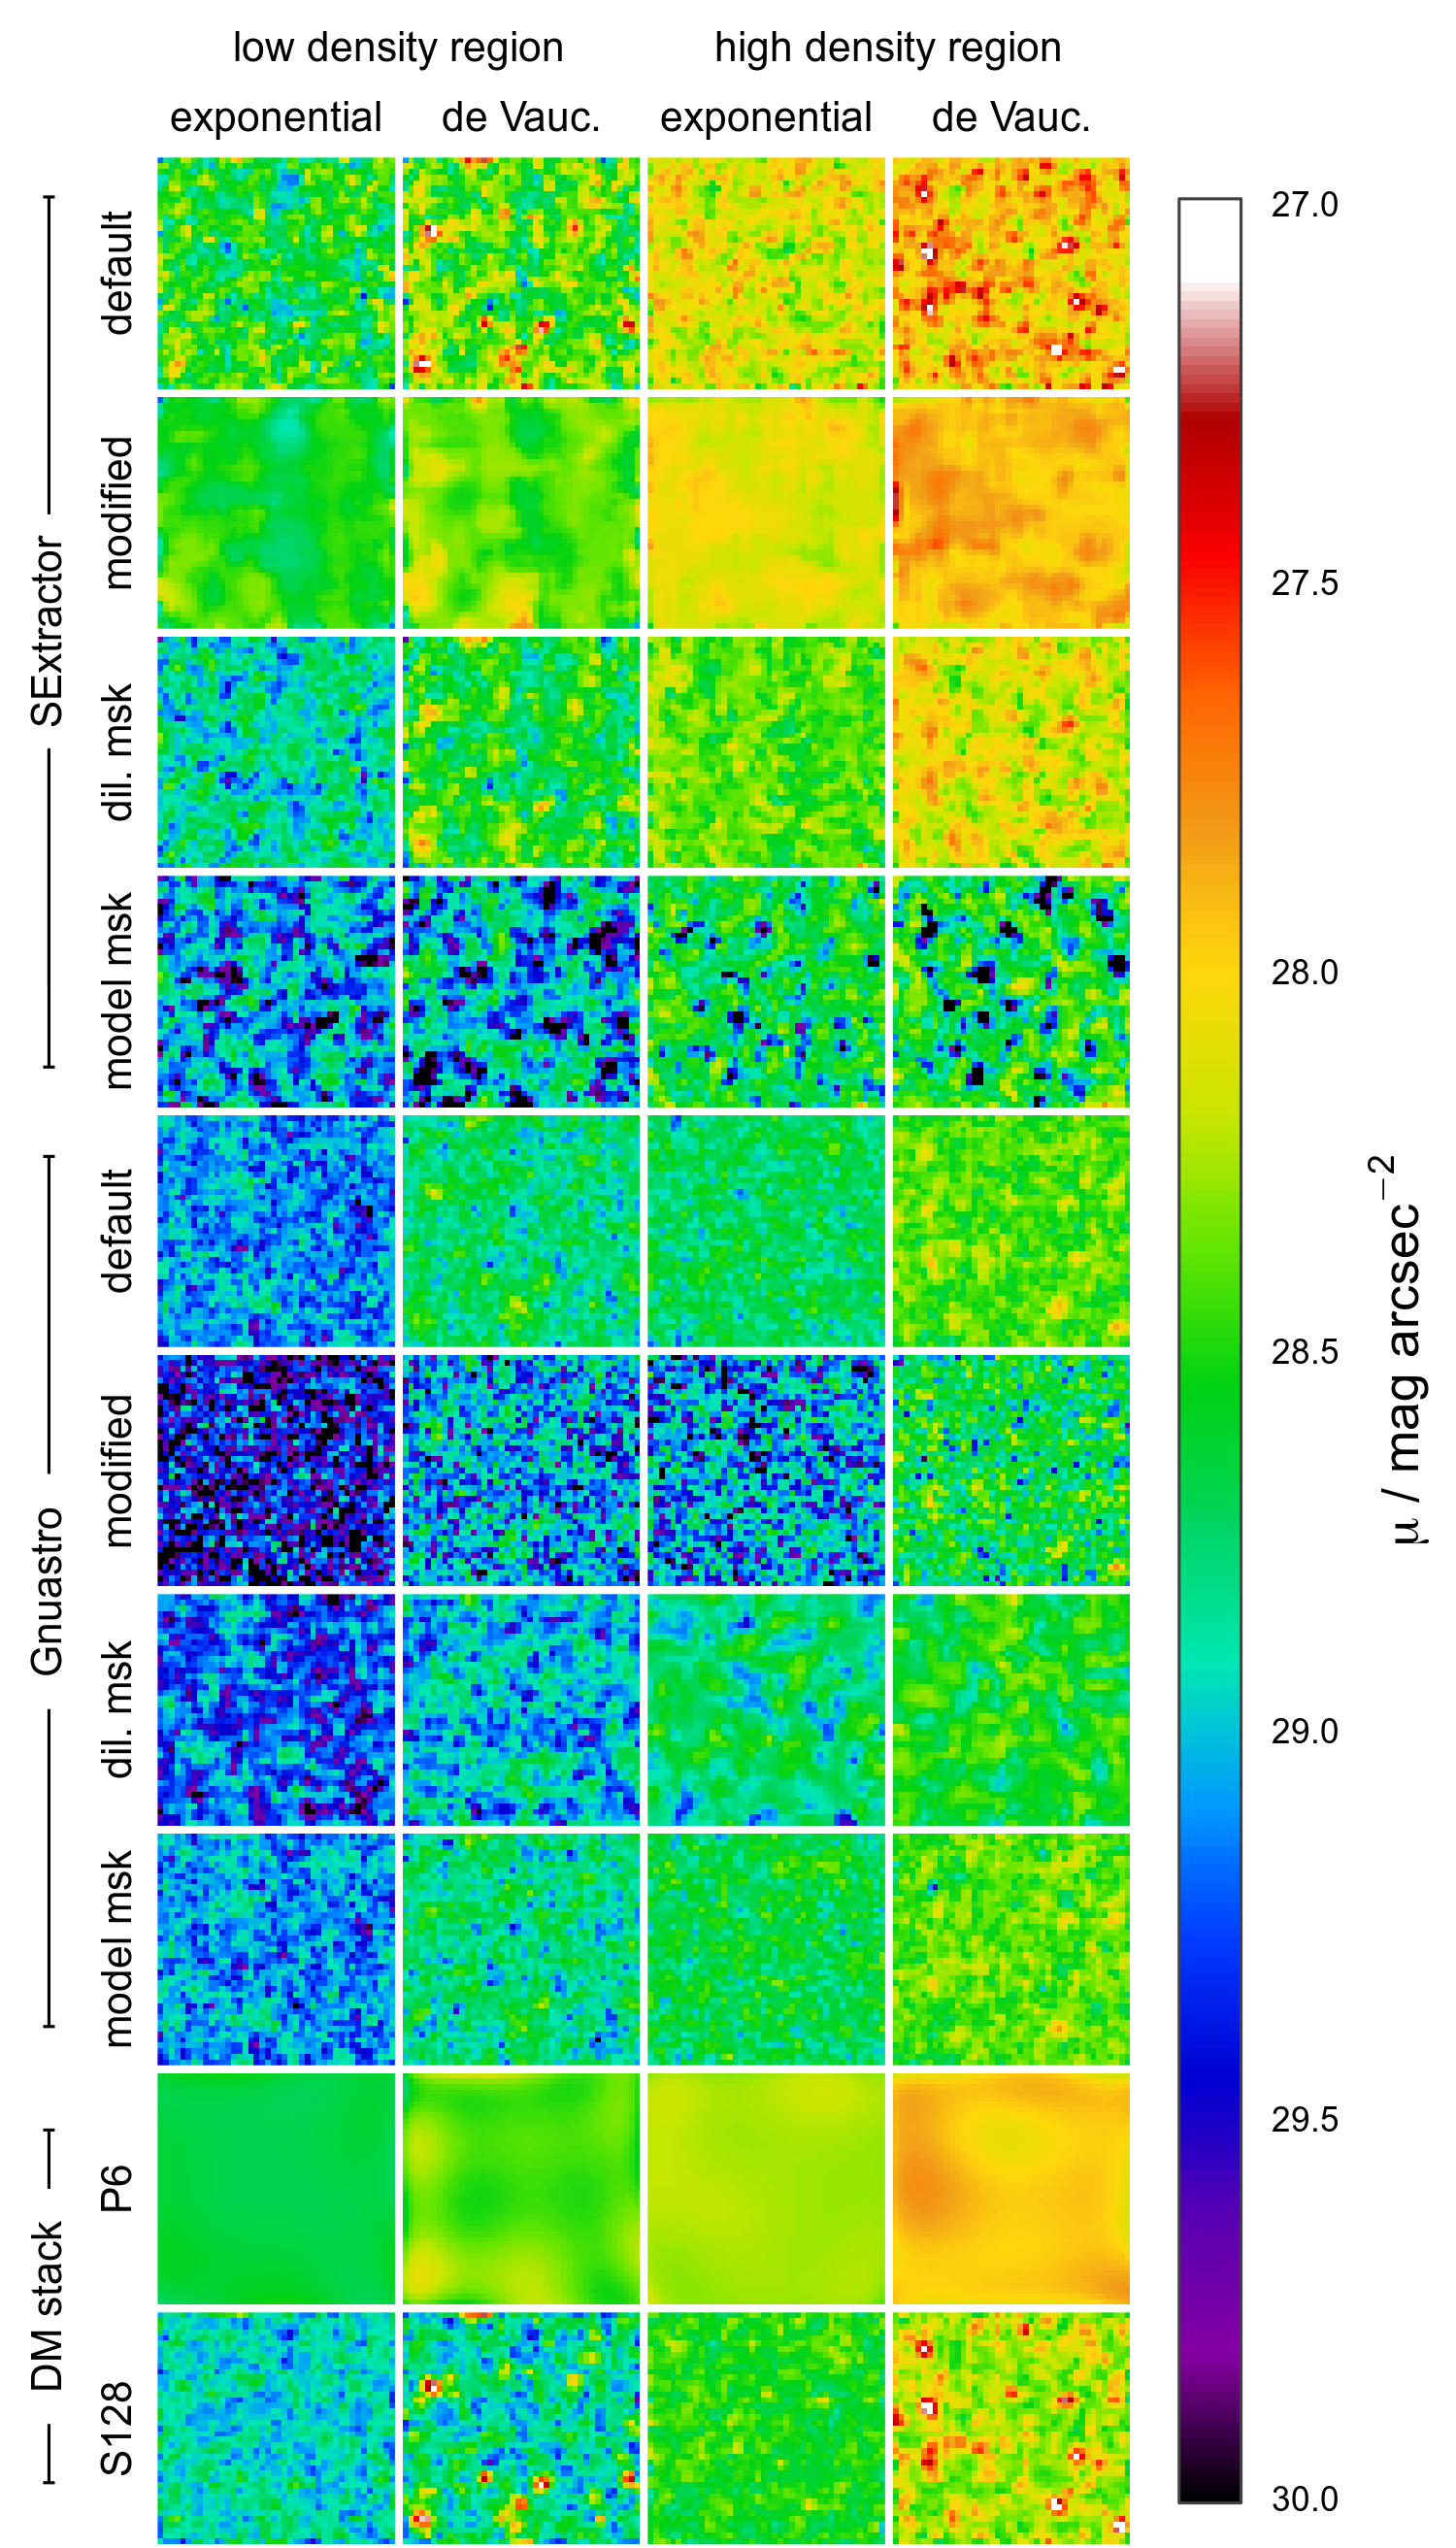
\includegraphics[width=\columnwidth]{{{fig/skymaps}}}
    \caption{Recovered background sky maps generated by various sky estimation and source extraction configurations. Rows depict different software configuration modes. Columns represent the recovered background sky maps generated from different input simulated datasets. Each original $4200\times4100$ pixel image has been binned into $100\times100$ pixel super-pixels and colour-coded according to its mean surface brightness value, as shown by the outlying colour bar. High density simulated regions tend on average to recover a brighter background sky level than their low density counterparts, owing to the greater number of contaminant sources littering the field. Similarly, simulated regions populated with extended de Vaucouleurs sources also recover brighter sky levels relative to their exponential source equivalents. Note how some sky estimation software configurations also recover a background sky with relatively fewer spatial fluctuations, an indicator that those particular configurations are less impacted by singular bright sources.}
    \label{fig:skymaps}
\end{figure}

Figure \ref{fig:skyvala} shows mean recovered sky levels in units of $\mathrm{mag\;arcsec}^{-2}$ as returned by all considered software configuration modes (see legend) and full simulated data type flavours (per panel). Software packages are uniquely colour coded, with \SExtractor results in orange, \Gnuastro results in purple, and \LSSTPs results in black. Background levels estimated from low density simulated data are shown in the two panels on the left, and their equivalents from high density regions are shown in the two panels on the right. The units along the $x$ axis are arbitrary, and serve only to separate out the points. Data points relating to modified, dilated masking and modelled masking are all based upon a default configuration (e.g., the dilated masking procedure is not based upon a modified configuration). Fields populated with exponential ($n=1$) sources are shown in the uppermost two panels, whilst fields populated with de Vaucouleurs ($n=4$) type sources are shown in the lower two panels. The global trends discussed above are also evident here, with the field density and profile type acting to modulate the resultant background level by up to an order of magnitude. As also shown in Table \ref{tab:results} and Figure \ref{fig:skymaps}, Figure \ref{fig:skyvala} additionally acts to highlight the variation in recovered background level as a function of specific software configuration. 

\begin{figure*}
    \centering
    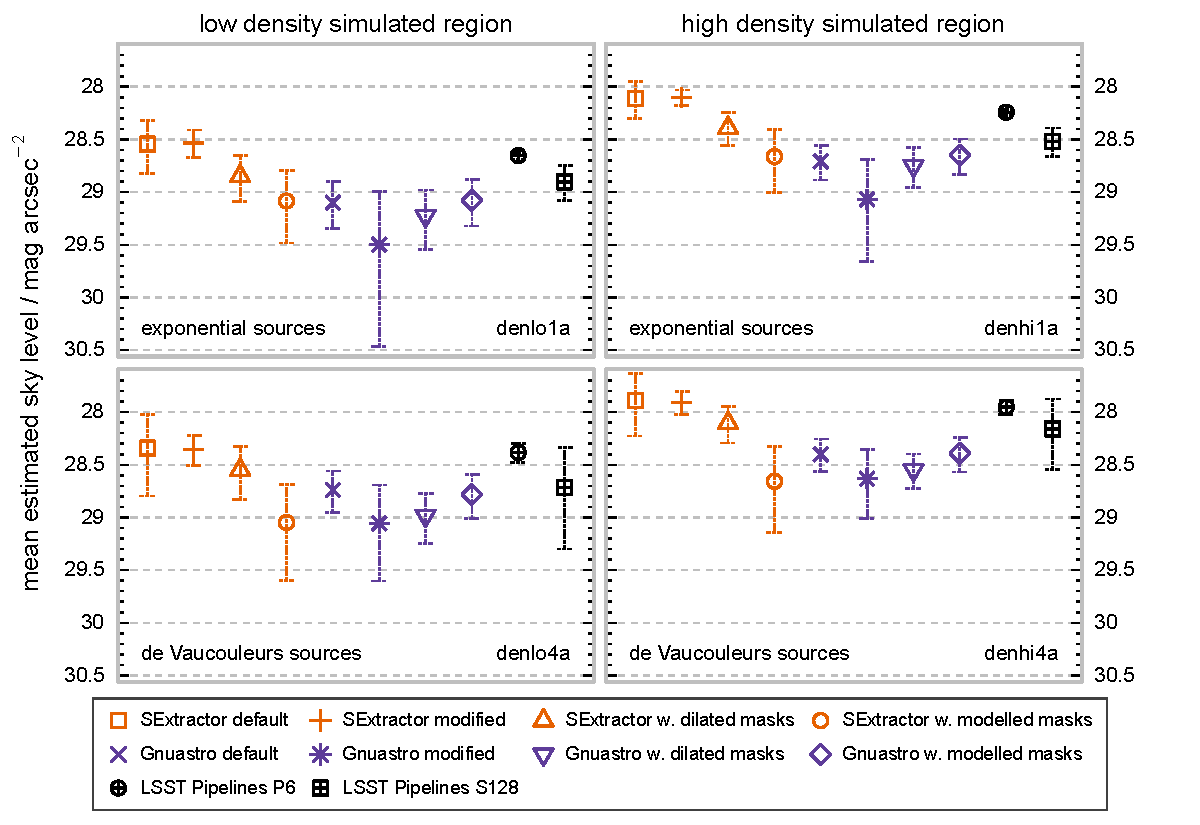
\includegraphics[width=0.9\textwidth]{{{fig/skyval-a}}}
    \caption{Mean estimated sky levels recovered for our complete simulated data as generated by \SExtractor (orange), \Gnuastro (purple) and the \LSSTPs (black) operating in various configurations (shown within the legend). Distinct software configuration modes are equally spaced along the x-axis within each panel, for clarity. The uppermost two panels represent simulated regions consisting of exponential ($n=1$) sources alone. The lower two panels represent simulated data consisting of de Vaucouleurs ($n=4$) sources alone. The left side panels represent low density simulated regions, whilst the right side panels represent high density simulated regions. Specific simulation data IDs are inset within each panel (see Table \ref{tab:simtab}). Error bars represent $\pm1\sigma$ about the mean. The impact of source density and source profile shape on the resultant sky level estimates shown here is evident, with higher density and extended source types (i.e., denhi4a) consistently brighter by up to an order of magnitude than that of their lower density or less extended simulated imaging counterparts. Various software configurations appear to consistently outperform others, with the discrepancy between the best and worst performing configurations similarly spanning an order of magnitude. The shape of sky level offsets between configurations appears relatively static as a function of field type, only varying in the overall amplitude.}
    \label{fig:skyvala}
\end{figure*}

\subsubsection{Trends by Software Configuration Mode}
\label{sec:mode}

Of the three software packages explored in this study, Figure \ref{fig:skyvala} shows that \Gnuastro consistently returns some of the faintest sky levels. With the notable exception of modelled masking (discussed below), sky recovered by \Gnuastro is of the order half a magnitude fainter than \SExtractor when comparing similar configuration setups. Further, \Gnuastro appears to return similar or fainter sky levels than even the \DMB iteration of the \LSSTPs. Such an obvious trend is likely a testament to the bottom-up approach towards source identification and characterisation employed by \Gnuastro, in contrast to the top-down flux thresholding techniques employed by \SExtractor and the \LSSTPs. 

Out of the box, default \SExtractor returns a sky which is brighter than default \Gnuastro outputs by approximately half a magnitude. The initial \DMA iteration of the \LSSTPs also performs comparably to both of these default runs, with a typical resultant sky level intermediate to the outputs given by \SExtractor and \Gnuastro. Improvements made to the \LSSTPs between \DMA and \DMB have improved on this typical sky level estimate by $\about0.25$ mag on average, placing it on par with default \Gnuastro outputs. 

The modifications made to \SExtractor do not appear to significantly alter its resultant output sky level relative to its default configuration. As a reminder, \SExtractor was modified by increasing the background mesh element size (and associated mesh filtering) within which sky is initially estimated, reducing the source detection threshold (i.e., allowing more flux to be classified as signal rather than noise), and making changes to the smoothing kernel and segmentation parameters. Many of these changes are often adopted in the literature to improve derived catalogue parameters, yet they appear to have had little to no impact on the resultant sky model. 

Conversely, the modifications made to \Gnuastro have significantly impacted its resultant sky model relative to its default configuration. As a brief reminder, adopted changes are to decrease the mesh size used within which initial background thresholding occurs, and to reduce the detection growth quantile threshold which defines how signal spills out into the noise. These changes combined have allowed for source profile footprints to more accurately map the faint LSB flux surrounding each object than had previously occurred. Relative to the default \Gnuastro configuration, modifications of this type improve the resultant background sky by up to half a magnitude. The \Gnuastro software package operating with a modified configuration produces some of the faintest background sky maps found in this study, fainter than \SExtractor and all iterations of the \LSSTPs for all input simulated data types. 

Application of the dilated masking technique to \SExtractor produces notable improvements to its output background maps, improving on default outputs by up to a quarter of a magnitude across all tested datasets. The magnitude-dependent dilated masking procedure employed here artificially expands the segmentation map around detected sources, bringing in more faint surrounding LSB flux which would otherwise have entered into the background model. This procedure has significant benefits, as explored in \citet{Ji2018}, helping reduce contamination at the background estimation step. Dilated masking also improves upon default \Gnuastro operational output, however, the improvement is more notable for background maps generated from low density simulated fields. Owing to the dense environments present in high density regions, the effect of dilated masking there is to further remove information from what was, already, a sparse dataset. In addition, dilated masking does act to reduce specific hot-spots which would otherwise be contaminated by singular bright sources (see Figure \ref{fig:dilmask_gnuastro} for an example of this).

Application of the modelled masking technique to these data produces a range of positive outputs, providing the single largest improvement to the overall mean sky level in the case of its use with \SExtractor. Modelled masking attempts to model a bright subset of the source detection catalogue with PSF-convolved single \Sersic profiles. The aim of this procedure is not to accurately model the core regions of these objects (as these will be masked from the sky estimation routine in any case) but rather to effectively model the flux drop-off into the noise in the wings of these sources. Modelled masking significantly improves the estimated sky level when applied to default \SExtractor sky estimation and source extraction routines, returning sky maps that are fainter in some cases by up to an order of magnitude. This is evidence for the fact that \SExtractor segmentation maps are typically not extensive enough, resulting in too much flux entering and contaminating the background model (e.g., see Figure \ref{fig:modmask_sex}). The benefit of modelled masking is that it does not reduce the number of pixels which ultimately enter the background estimation routine, a significant advantage over the dilated masking procedure and in crowded fields. In contrast to these strong positive results observed with \SExtractor outputs, modelled masking as applied to \Gnuastro default outputs do not appear to improve upon the global mean sky levels in any meaningful manner, producing similar outputs to that found by default. As evidenced in Figure \ref{fig:modmask_gnuastro}, this is likely due to the fact that default \Gnuastro segmented regions are already fairly extensive, and therefore not in need of any further major adaptions. As with dilated masking however, modelled masking still acts to improve specific hot-spots which would otherwise have been contaminated by singular bright sources.

\subsubsection{Trends in Output Source Catalogue Fidelity}
\label{sec:fidelity}

Whilst the previous sections have focused on analysis of the output sky models, the fidelity of the resultant source catalogues must also be of interest. To facilitate this analysis we generate a series of matched catalogues for each data output produced here, matching the output catalogue to the known simulated input catalogue using the \texttt{STILTS}\footnote{\url{http://www.star.bris.ac.uk/~mbt/stilts}} software package. We perform a 3-dimensional match between the output and input catalogues based upon $x$ and $y$ pixel coordinates and total magnitude. To match, the output pixel coordinate must be within $5$ pixels of its input location (independently on both axes), and the output magnitude must be within $0.5$ magnitudes of the input magnitude. Magnitude estimates are derived from the Kron-like $\mathrm{FLUX\_AUTO}$ value with \SExtractor outputs, the $\mathrm{BRIGHTNESS}$ value with \Gnuastro outputs, and the $\mathrm{base\_SdssShape\_instFlux}$ value with \LSSTPs outputs. Figure \ref{fig:ndetnmatcha} shows the number of true matched objects ($y$-axis) as a function of the total number of detected objects ($x$-axis) for various software configuration modes listed in the legend and simulated data type flavours. Data point type and colour coding is identical to that previously used. Slanted dashed grey lines represent different fidelity fractions, as indicated. 

\begin{figure*}
    \centering
    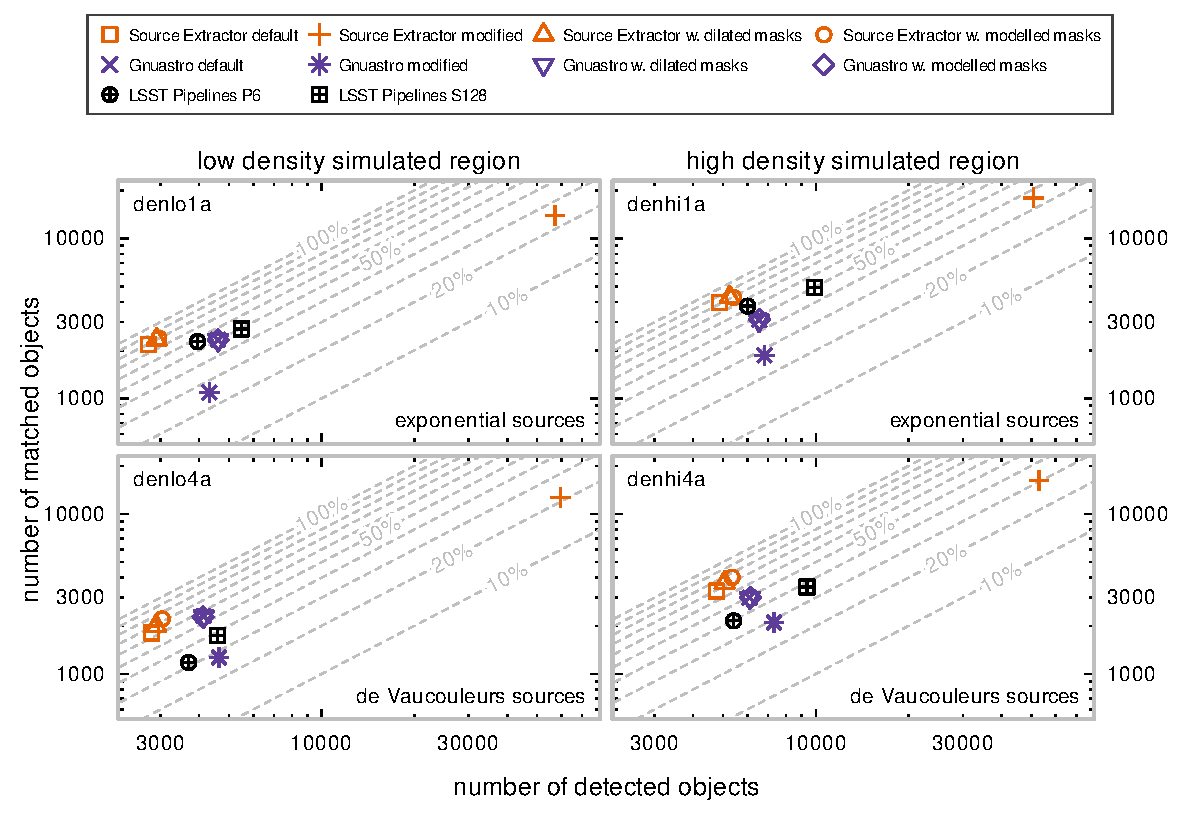
\includegraphics[width=0.9\textwidth]{{{fig/ndetnmatch-a}}}
    \caption{Number of true matched objects as a function of the total number of detected objects given by the various sky estimation and source extraction software configuration modes listed in the legend. Output sources are matched to their corresponding simulated input counterpart if they satisfy three criteria: the $x$ and $y$ output pixel positions fall within $5$ pixels of the input source and the recovered magnitude is within $\pm0.5$ mag of its input total magnitude. Dashed grey lines represent boundaries equivalent to 100\%, 50\%, 20\% and 10\% matched to total ratios. The \SExtractor outputs typically return the highest fidelity ratios, with \Gnuastro and the \LSSTPs instead leaning towards recovery of more objects.}
    \label{fig:ndetnmatcha}
\end{figure*}

We find that \SExtractor default modes of operation (i.e., default, dilated masking and modelled masking) produce the highest fidelity catalogues, with approximately two thirds of their output catalogues finding a corresponding true match in their equivalent original input catalogues. These catalogues also return the fewest total number of objects however, indicating that default \SExtractor is well optimised towards returning the lowest-hanging fruit in any given field of view. Modified \SExtractor operations drastically increase both the total number of output sources (by a factor of $\about20$) and the number of matched sources (by a factor of $\about10$), with a reduced fidelity ratio of around one third.

Default \Gnuastro operational modes (i.e., default, dilated masking and modelled masking) similarly cluster together, with a matched fidelity ratio of around $50\%$. These outputs do find a larger number of total sources than their equivalent \SExtractor runs, however, fewer of these are able to be matched to a known simulated input. Modifications made to \Gnuastro act to somewhat increase the total number of detected objects (by $\about10\%$, excepting in the denlo1a scenario where no significant increase is recorded), however, any increase is at the expense of source fidelity, with a drastically reduced recovered fidelity ratio of $\about20\%$ or lower.

The two \LSSTPs modes of operation perform fairly consistently and comparably to the default \Gnuastro outputs, returning fidelity ratios in the range $\about30\%$ to $\about50\%$. Simulated regions populated with exponential sources tend to lead to higher fidelity output \LSSTPs catalogues on average, with a larger number of spurious sources for no discernible increase in total numbers found in the equivalent de Vaucouleurs populated fields. Progressing from the \DMA mode of operation to the \DMB variant approximately maintains a similar fidelity level, improving in both total number of detected objects and the equivalent number of true matched sources.

In addition to overall numbers, we also want to explore whether the output magnitudes being returned by our software package of choice accurately portray the true input magnitudes in our simulated datasets. Figure \ref{fig:lumfrac} shows median recovered luminosity fractions for the matched source subsets described above. The $x$-axis shows the median recovered luminosity fraction $f$ for all matched sources, where $f=\mathrm{median}(\mathrm{L}_{\mathrm{out}}/\mathrm{L}_{\mathrm{in}})$. The $y$-axis represents the median recovered luminosity fraction for the 25 largest matched sources alone ($f_{25}$). The latter of these two parameters is of particular interest, as these sources have the largest individual impact on background sky estimation results. We find a strong bimodality in $f$ as a function of source profile type, as might naively be expected, with similar overall trends observed in both regardless of field density. 

\begin{figure*}
    \centering
    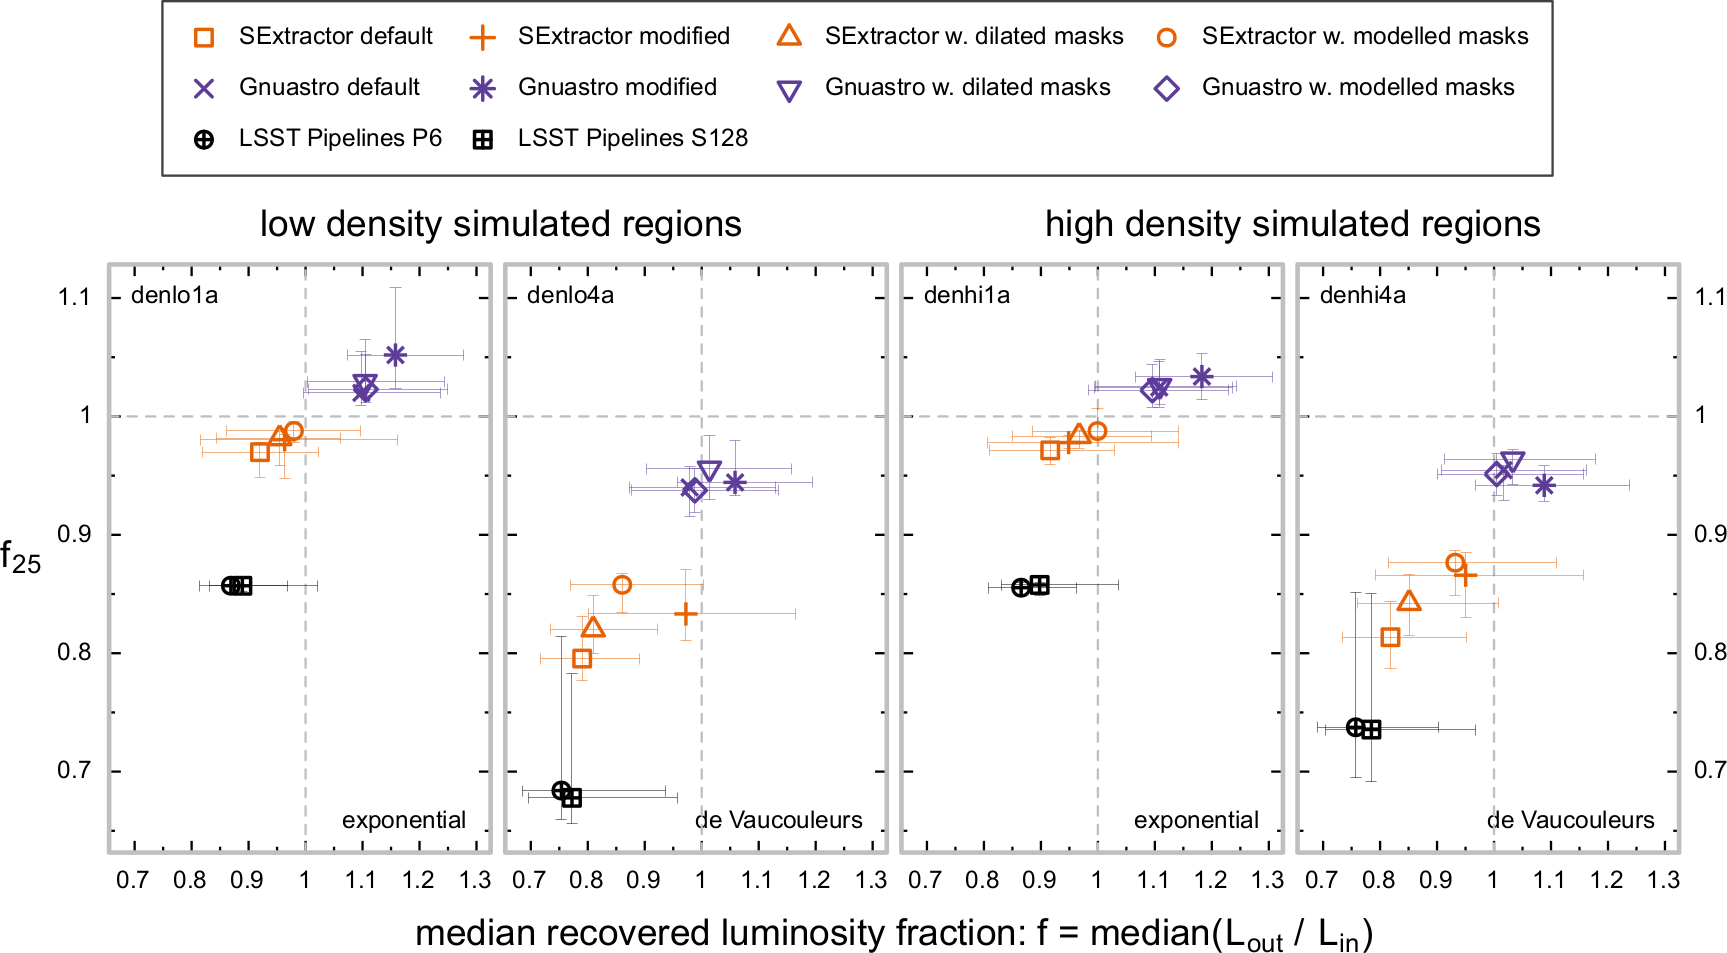
\includegraphics[width=1\textwidth]{{{fig/lumfrac}}}
    \caption{Median recovered luminosity fractions (output/input) for matched sources as determined by various source extraction techniques listed in the accompanying legend. Each panel represents a different simulated input dataset, as indicated by the supporting label text. Within each panel, the $x$-axis represents the median recovered luminosity fraction $f$ for all matched sources, where $f=\mathrm{median}(\mathrm{L}_{\mathrm{out}}/\mathrm{L}_{\mathrm{in}})$, whilst the $y$-axis represents the median recovered luminosity fraction for the 25 largest sources alone ($f_{25}$, i.e., those sources that have the largest impact on background sky estimation and are equivalently most severely impacted by it). Error bars represent $25^{\mathrm{th}}$ and $75^{\mathrm{th}}$ percentile ranges. These results show that \SExtractor performs well with exponential type sources, correctly recovering close to $100\%$ of the simulated input flux, whilst under-estimating total flux for the more extended de Vaucouleurs type sources by $\about15\%$. Conversely, \Gnuastro performs well for the majority of de Vaucouleurs types, but does miss $\about5\%$ of the flux for the largest de Vaucouleurs type sources, and incorrectly over-estimating flux for exponential types sources by at least $10\%$.}
    \label{fig:lumfrac}
\end{figure*}

Here it becomes apparent that \SExtractor appears optimally configured for the accurate characterisation of exponential type sources, with all \SExtractor software variants clustering just below $f=1$ and $f_{25}=1$, i.e., their median output luminosities accurately represent their inputs. In sharp contrast to this, \SExtractor results for de Vaucouleurs populated fields are much less consistent. Typical median recovered luminosity fractions for de Vaucouleurs type sources in both field density regimes return $f\sim0.85$ (and equivalently for the largest 25 sources), i.e., $\about15\%$ of their input flux is missing in its output flux estimate. The value of $f$ varies significantly with \SExtractor software configuration, with the default mode of operation performing worst, and the modified and modelled masking procedures performing significantly better on average. Several such configuration modes push the \SExtractor results up to $f\sim0.95$, however, all continue to struggle for the largest 25 sources.

Conversely, the \Gnuastro package appears designed for more optimal extraction of de Vaucouleurs type sources, more accurately picking up the LSB flux in the wings of these objects. All configuration variants of \Gnuastro return $f\sim1$ in the case of de Vaucouleurs type simulated datasets. The recovered flux for the 25 largest sources however falls somewhat lower, at $f_{25}\sim0.95$ (i.e., the brightest 25 sources are reported to be $\about5\%$ fainter than their true input \Sersic magnitude). This in-built facility to identify LSB flux around de Vaucouleurs sources does not similarly lead to a successful outcome in the case of exponential-type populated fields. Recovered exponential source flux appears to be over-estimated by $\about10\%$ (and $\about15\%$ in the case of a modified \Gnuastro configuration). It appears that \Gnuastro tends towards inaccurately incorporating flux from surrounding faint EBL sources and noise spikes into these exponential source footprints, falsely inflating their resultant flux estimates. 

Of all three software packages explored here, results from the \LSSTPs consistently recover the lowest flux estimates. In the exponential scenario, recovered fluxes are $\about10\%$ lower then their known inputs. When considering the largest 25 sources alone, recovered fluxes are $\about15\%$ lower than their known inputs. The situation is notably worse in the case of fields populated with de Vaucouleurs sources, with equivalent recovered values of $f\sim0.8$ and $f_{25}\sim0.7$, respectively. This indicates that a significant amount of flux from these sources is leaking into the resultant sky estimate, severely contaminating resultant sky maps.

\section{Conclusions}
\label{sec:conclusions}

% INTRODUCTION
As we enter an era whereby deep, wide-area astronomical imaging surveys are rapidly becoming the new normal, the possibilities for exploring novel and exciting avenues of science are vast. One such topic is in the field of low surface brightness (LSB) astronomy. The LSB Universe encodes a wealth of information on the history of mass assembly across a broad range of scales, from some of the largest gravitationally bound structures known, the Intra-Cluster Medium, to some of the smallest and faintest, LSB dwarf galaxies, and much in between. As imaging surveys begin mapping such parameter space down to sufficient depth on a regular basis, we are now able to build up statistically significant catalogues of such structures for the first time, ultimately allowing for their classification and characterisation. However, many of the traditional tools developed by astronomers to reduce and process acquired datasets have proven to be inadequate when it comes to handling LSB data. In particular, many widely used methods of sky estimation and subtraction leave much of this LSB light at significant risk, either severely compromising it during image processing or, at worst, destroying it. 

% PROJECT OVERVIEW
In this paper we explore multiple techniques towards mitigating such sky over-subtraction during image processing. To achieve this, we generate detailed simulated imaging based upon real data, and run these mock images through several different image processing configurations. We adopt the Hyper Suprime-Cam Subaru Strategic Program \citep[HSC-SSP,][]{Miyazaki2012,Miyazaki2018,Aihara2018a} as our reference dataset, owing to its significant depth (a typical $5\sigma$ point source depth of $r\about26$ mag.) and wide-scale usage amongst the LSB community. In addition, HSC-SSP data is being reduced by the \RO \LSSTPs \citep{Juric2017,Bosch2018,Huang2018}, a unified image processing pipeline designed for use with future \RO \LSST (LSST) `deep, wide and fast' survey data. 

% DATA SETUP
Two proto-typical patches of sky are selected from the HSC-SSP PDR1 dataset \citep{Aihara2018b}, one each to represent both a low-density field and a high-density field. These chosen tract-patch regions measure approximately $700\times700$ arcseconds in dimension, with a pixel scale of $0.168$ arcseconds per pixel. We derive a measure of the point spread function for these data, and generate estimates of initial sky statistics prior to sky subtraction. Using this information, we use the \GalSim image simulation software package \citep{Rowe2015} to generate mock simulated imaging closely mimicking these two regions. Each region is subsequently populated by a range of PSF-convolved \Sersic profiles. The intrinsic properties for each \Sersic source are carefully defined to maintain the distributions initially derived from our adopted HSC-SSP dataset, such as magnitude, half-light radius, and field clustering signature. To explore any variation with \Sersic profile shape, we simulate each region twice: once with each source described by an exponential $n=1$ \Sersic profile, and again with each source described by a de Vaucouleurs $n=4$ \Sersic profile. In addition, we generate two further variants for each simulated image by limiting the number of sources according to a flux-threshold: first with all detected and expected sources down to a total apparent $r$-band magnitude of $m_r=30$ mag, and second taking only a subset of these sources which might typically be detected during an actual observational run. This second flux-limited sample essentially excludes sources which normally contribute to the faint extragalactic background light (EBL). As a result of these definitions, we are ultimately left with three binary simulated image configurations: two field density variants; two \Sersic profile shape variants; and two flux-limited sample variants. The result of this is the generation of eight simulated mock regions upon which to test various sky-estimation techniques. 

% SOFTWARE SETUP
Three contemporary software packages that perform sky estimation and source detection are explored here: \SExtractor \citep{Bertin1996}; \Gnuastro \citep{Akhlaghi2015}; and the \LSSTPs \citep{Bosch2018,Bosch2019}. These software packages have been chosen owing to their wide usage amongst the astronomy community at large, or (in the case of the \LSSTPs) their expected importance in the reduction of future LSB datasets. We process all eight simulated datasets using each software package in a series of specific configurations, extracting metrics for performance in both sky estimation and source extraction capabilities. Both \SExtractor and \Gnuastro are operated in four different configurations: default, modified, with dilated masking, and with modelled masking. Default modes of operation are designed to gauge how the software performs `out-of-the-box'. This provides a useful baseline comparison, however, modifications to the setup configuration are normally desirable to facilitate the needs of a specific science case. Our modified modes of operation mimic such typical modifications, including varying the box size within which sky estimation and source characterisation occurs and changing the detection threshold for distinguishing sources from noise. The dilated masking procedure closely matches the approach previously outlined in \citet{Ji2018}. In brief, an initial default detection phase is performed, and output detection footprint masks are artificially expanded according to the estimated magnitude of the underlying source. A subsequent sky estimation and source detection step is performed using these expanded masks. The modelled masking procedure is a novel variation on this approach. Instead of dilating detection masks, a simple one-component fitted \Sersic profile is subtracted from each initially detected source before performing a second round of sky estimation and source detection. Finally, the \LSSTPs is operated in two different configurations: first to estimate and model the subtracted sky using a sixth degree polynomial (\DMA), and second to use a more local $128$-pixel spline fitting procedure instead (\DMB). 

% SKY RESULTS BY DATA TYPE
The most optimal sky estimation results are achieved with data which is comprised of low density exponential-type sources and whereby all faint EBL sources have been accounted for and excluded. Including EBL sources increases the resultant background sky estimate by $\Delta{f}_{\mathrm{a}-\mathrm{b}}=3.20\pm0.74$ $e^{-}/\textrm{pixel}$, when averaged across all software configurations explored here. This evidences not only the importance of accounting for such sources in the first instance, but also the significant impact they can have on LSB science. Increasing the source field density from a typical low-density region to a high-density region similarly increases the resultant sky estimate, in this case by an average of $\Delta{f}_{\mathrm{hi}-\mathrm{lo}}=0.91\pm0.81$ $e^{-}/\textrm{pixel}$. A higher source density reduces the total number of available pixels which may ultimately be used for sky estimation, leading to more flux inadvertently leaking into the sky map and contributing to contamination of the sky estimate. Switching from a region populated with exponential-type sources to one populated with de Vaucouleurs type sources likewise increases the resultant estimated sky level by $\Delta{f}_{\mathrm{4}-\mathrm{1}}=0.73\pm0.45$ $e^{-}/\textrm{pixel}$. Such sources contain broad extended wings, and typical flux-thresholding sky estimation techniques inaccurately attribute much of the faint flux in these wings to the sky, rather than to its host source.

% SKY RESULTS BY DEFAULT SOFTWARE CONFIGURATION
Across all simulated datasets utilised here, the \Gnuastro software package consistently returns the most optimal sky estimation results. Operating in default upon full simulated datasets (i.e., including EBL), \Gnuastro is able to generate mean sky levels in the range $\about28.5\;\mathrm{mag\;arcsec}^{-2}$ to $\about29\;\mathrm{mag\;arcsec}^{-2}$ (varying according to input simulated data type as discussed above). By contrast, default \SExtractor runs achieve mean sky levels in the range $\about28\;\mathrm{mag\;arcsec}^{-2}$ to $\about28.5\;\mathrm{mag\;arcsec}^{-2}$, i.e., $\about0.5\;\mathrm{mag\;arcsec}^{-2}$ brighter than \Gnuastro. The scatter with simulated input data type between these two default runs appears to be relatively consistent. The \DMA variant of the \LSSTPs performs similarly to default \SExtractor, albeit with tighter scatter in magnitude as a function of data type. Conversely, the \DMB variant of the \LSSTPs performs similarly to the default \Gnuastro runs, achieving sky level estimates about half a magnitude fainter than its \DMA counterpart yet with an increased scatter as a function of data type. One further significant difference to note is in the spatial frequency of output sky maps. Both \SExtractor, \Gnuastro and \DMB return relatively high-frequency sky maps, more suited towards local sky estimation tasks and yet more easily contaminated by singular bright sources. The \DMA configuration typically returns a much flatter low-frequency map, more suited towards flat sky-pedestal estimation. 

% SKY RESULTS BY MODIFIED CONFIGURATIONS
Typical modifications made to the operation of \SExtractor have little effect on its resultant sky level, returning sky levels comparable to that of its default mode of operation, albeit with a tighter scatter. Conversely, modifications to \Gnuastro have a notable impact on resulatant sky levels, with average recovered values in the range $\about28.5\;\mathrm{mag\;arcsec}^{-2}$ to $\about29.5\;\mathrm{mag\;arcsec}^{-2}$. The largest gains relative to a default mode of operation are made in the case of fields comprised of exponential sources. These sky results are the faintest recovered during this study, however, they also exhibit the largest scatter. Further considerations, such as how these modifications impact resultant source catalogues, are reviewed below. 

% SKY RESULTS BY DILATED MASKING
The magnitude-dependent dilated masking procedures applied here are able to effectively block out most of the contaminant flux which would otherwise bias high any resultant sky estimate. The largest improvements appear to be in the case of \SExtractor, with output sky maps $\about0.25\;\mathrm{mag\;arcsec}^{-2}$ fainter than their default outputs. Improvements are also found in the case of \Gnuastro outputs, albeit to a lesser degree, with recovered sky levels fainter by $\le0.25\;\mathrm{mag\;arcsec}^{-2}$. Dilated masking appears to be a solid and dependable procedure, severely lessening the impact of over-subtraction in the wings of bright sources and producing significantly improved background sky estimates across the field. However, as evidenced in Figure \ref{fig:dilmask_sex} and Figure \ref{fig:dilmask_gnuastro}, dilated masking procedures also reduce the overall number of available pixels with which to construct a background sky model. In an era of increasingly deep sky surveys with ever increasing source densities, losing such a large fraction of sky pixels may quickly become untenable. 

% SKY RESULTS BY MODELLED MASKING
As with the dilated masking procedure discussed above, the modelled masking procedure outlined here is also able to successfully remove much of the contaminant flux well into the noise, and consequently helps in recovering a fainter and more accurate sky statistic. In the case of \SExtractor outputs, the application of modelled masking improves the resultant sky estimate by anywhere from $\about0.5\;\mathrm{mag\;arcsec}^{-2}$ to $\about1\;\mathrm{mag\;arcsec}^{-2}$ fainter than their equivalent default outputs. Indeed, \SExtractor outputs appear well suited towards the application of this procedure, producing some of the largest magnitude gains found in this study. Conversely, modelled masking has little impact on data processed by \Gnuastro. The cause of this appears linked to the already extensive source masks produced by \Gnuastro, likely owing to the bottom-up approach that package utilises towards source and noise characterisation, leaving little extra work for a modelled mask to do. Modelled masking is an exceedingly promising methodology which may easily be applied to existing flux-threshold-based data analysis pipelines. Not only does it succeed in recovering a fainter and more accurate sky map, but it also increases the total number of pixels available for any subsequent sky estimation relative to the aforementioned dilated masking procedure. 

% NOTES ON CATALOGUE FIDELITY RATIOS
In addition to sky level accuracy, this study has also compared the quality of output catalogues produced via the various methods discussed above using two distinct indicators. The first is to compare output catalogue number fidelity values, i.e., how many objects in total are detected subsequent to the sky estimation procedures utilised here, and of these sources, how many can be directly attributed back to a known simulated input source. On the whole, outputs in this parameter space tend to cluster as a function of software type. Outputs from \SExtractor tend to recover fidelity ratios of the order $\about66\%$. The notable outlier is in the modified \SExtractor case, whereby the fidelity ratio has dropped to $\about33\%$, yet recovers an order of magnitude or more sources. Outputs from \Gnuastro return fidelity ratios of the order $\about50\%$. As with \SExtractor, the modified \Gnuastro case is a notable outlier, reducing the fidelity ratio to $\about15\%$ whilst recording only a minor increase in the total number of detected objects. The two \LSSTPs configurations return fidelity ratios in the range $\about40\%$ to $\about50\%$, with the higher values in the case of fields populated by exponential sources. The \DMB variant of the \LSSTPs does recover more sources (and matched sources) than \DMA, with only a minimal change in fidelity ratio recorded. 

% NOTES ON CATALOGUE RECOVERED LUMINOSITY FRACTIONS
The second and final catalogue quality indicator explored here is to compare the output recorded magnitude for each source with its known simulated input magnitude as a function of software configuration mode. In general, we find that the \SExtractor package appears well optimised towards accurately recovering the flux of exponential type sources, recovering luminosity fractions of the order unity in both low density and high density regions. Importantly, this statistic remains close to unity whether considering the entire matched population, or when only considering the largest $25$ sources. Conversely, for these exponential-type data \Gnuastro tends to over-estimate the recovered flux by $\about10\%$ when aggregated across all sources (this value is several percent higher when using a modified configuration setup). The flux over-estimation is less when only considering the largest $25$ sources, of the order $\about\mathrm{few}\%$. With the same data, both variants of the \LSSTPs tend to underestimate the recovered flux of exponential sources, by $\about15\%$ (for both the entire aggregated matched population and the largest $25$ subset). With regards the more extended de Vaucouleurs type sources, \Gnuastro performs much more strongly, recovering an aggregated population mean luminosity fraction of the order unity. When considering the largest $25$ sources however, \Gnuastro still returns $\about5\%$ less flux than had initially been input. All other software modes significantly under-estimate the recovered flux in the case of fields populated by de Vaucouleurs type sources (for both the entire aggregated population and the largest $25$ subset), with \SExtractor returning fluxes that are $\about15\%$ fainter than had initially been input, and the \LSSTPs variants returning fluxes that are $\about25\%$ fainter than had initially been input. These results underline the importance of considering what impact modifications to sky estimation routines will ultimately have on the resultant output science catalogues.

% SUMMARY
In conclusion, this study has explored various means by which the sky may be estimated in contemporary astronomical imaging. It is clear that each method utilised here, and each software package used to reduce these simulated datasets, has both strengths and weaknesses. Some software packages are more optimised towards reduction of shallow data, others towards crowded fields, and others yet towards the production of high fidelity output catalogues. Similarly, some image processing methodologies are more suited towards extraction of more compact sources, others towards accurately mapping the faint extended wings of de Vaucouleurs type radial profiles. The `bottom-up' approach towards source detection and sky estimation employed by \Gnuastro appears to have merits, accurately identifying faint flux and attributing it to bright sources well out into the noise, therefore significantly aiding in the recovery of extremely faint sky levels. However, this same routine generates vast detection footprint maps that exclude significant portions of the input dataset, perhaps making it inappropriate for future high-density deep imaging surveys. Conversely, the `bottom-up' approaches of \SExtractor and the \LSSTPs seemingly lend themselves towards greater configurational possibilities, with the former successfully utilising the modelled masking procedure to recover background sky levels of the order that produced by \Gnuastro, yet requiring significantly smaller detection footprints. Both such packages struggle however to accurately recover all of the flux for more extended de Vaucouleurs type sources, highlighting the difficulty of accurately ascribing flux within noise. Of all the sky estimation variants explored here, both dilated masking and modelled masking perform strongly. Each is able to be trivially added to existing image processing pipelines, producing a notable improvement on resultant sky levels and improving output science catalogue fidelity in the process. Long term, we believe the modelled masking procedure presented here should be the preferred of the two, due in large part to its capacity to handle extremely dense and deep datasets whilst producing superior estimated sky outputs. An application of the modelled masking procedure presented here to an image processing pipeline such as the \LSSTPs when processing future \RO imaging would therefore be of significant benefit, not only to the LSB science community but to the entire scientific user base as a whole. 

\newpage
\section*{Acknowledgements}
\label{sec:acknowledgements}

This material is based upon work supported in part by the National Science Foundation (NSF) through Cooperative Agreement 1258333 managed by the Association of Universities for Research in Astronomy (AURA), and the Department of Energy under Contract No. DE-AC02-76SF00515 with the SLAC National Accelerator Laboratory. Additional funding for Rubin Observatory comes from private donations, grants to universities, and in-kind support from LSSTC Institutional Members.
This research was also supported by Department of Energy grant DE-SC0009999 and NSF/AURA grant N56981C.

%%%%%%%%%%%%%%%%%%%%%%%%%%%%%%%%%%%%%%%%%%%%%%%%%%

%%%%%%%%%%%%%%%%%%%% REFERENCES %%%%%%%%%%%%%%%%%%

\bibliographystyle{mnras}
\bibliography{bibtex}

%%%%%%%%%%%%%%%%%%%%%%%%%%%%%%%%%%%%%%%%%%%%%%%%%%

%%%%%%%%%%%%%%%%% APPENDICES %%%%%%%%%%%%%%%%%%%%%

\appendix

\section{Threshold Levels}
\label{sec:thresholds}

To facilitate a fair comparison of detected source catalogues generated from each of our $57$ input sky-subtracted fields, we require a uniform absolute detection threshold to use as an input to \SExtractor. The default operation of \SExtractor identifies sources as contiguous regions of flux lying above some relative threshold level, normally $1.5\sigma$ above the locally determined sky. As sky estimation varies across fields, the resultant threshold level will also vary, therefore precluding our use of the default \SExtractor configuration in this case. 

To estimate a global absolute threshold level, we initially ran \SExtractor in default mode on each of the $57$ fields. The resultant $1.5\sigma$ threshold levels in counts are shown in the histogram in Figure \ref{fig:threshlvls}. Individual field values are shown in the underlying rug plot. As can be seen, our threshold levels vary from $\about0.06$ counts to $\about0.1$ counts, peaking at $\about0.07$ counts. We choose this peak value of $0.07$ counts as our global absolute threshold level with which to subsequently generate our source detection catalogues with the \SExtractor software package. 

\begin{figure}
    \centering
    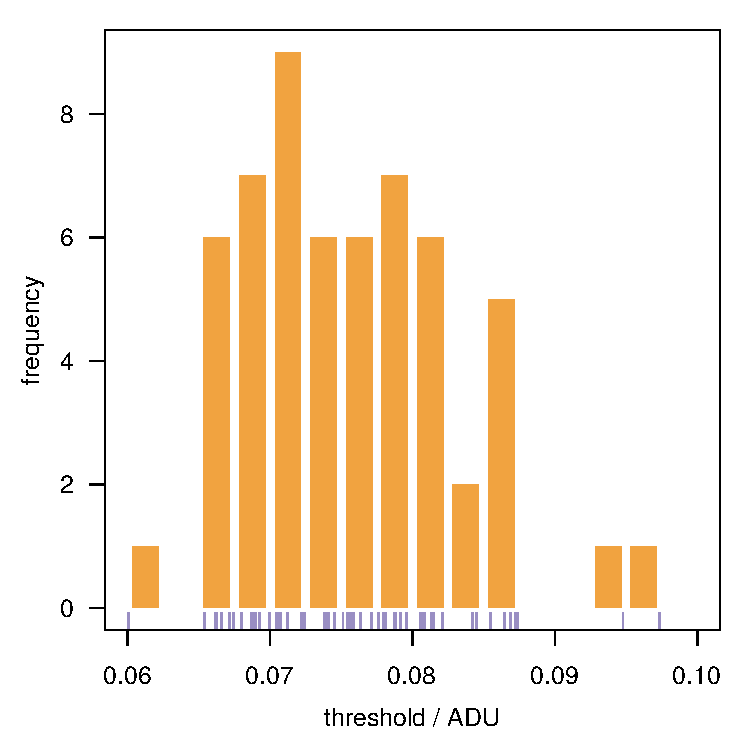
\includegraphics[width=\columnwidth]{{{fig/threshlvls}}}
    \caption{Histogram showing relative $1.5\sigma$ detection threshold levels as output by \SExtractor when operated in default mode upon each of our $57$ input fields. Individual field values are shown in the underlying rug plot. We adopt a threshold level of $0.07$ counts as our global absolute detection threshold level, corresponding to the approximate position of the peak in this figure.}
    \label{fig:threshlvls}
\end{figure}

\section{\GalSim Input Catalogues}
\label{sec:inputcats}

Table \ref{tab:simcat} shows an excerpt from the input catalogue produced for the exponential ($n=1$) simulation of the low density region. Here we show the five brightest sources out of a total of $428257$ objects in this density regime. Columns, from left to right, are: $x$ pixel position in the field; $y$ pixel position in the field; total source flux; half light radius $R_e$; axis ratio ($q=b/a$); position angle; \Sersic index $n$; and, postage stamp size. Associated units (where appropriate) are shown beneath column headers in parentheses. Parameter values are rounded to a varying number of decimal places, as shown. 

\begin{table}
    \setlength{\tabcolsep}{2.5pt}
    \begin{tabular}{ r | r | r | r | r | r | r | r }
    \multicolumn{1}{c}{$x$} & \multicolumn{1}{c}{$y$} & \multicolumn{1}{c}{flux} & \multicolumn{1}{c}{$R_e$} & \multicolumn{1}{c}{$q$} & \multicolumn{1}{c}{P.A.} & \multicolumn{1}{c}{$n$} & \multicolumn{1}{c}{stamp size}\\
    \multicolumn{1}{c}{(pix)} & \multicolumn{1}{c}{(pix)} & \multicolumn{1}{c}{(counts)} & \multicolumn{1}{c}{(pix)} & \multicolumn{1}{c}{ } & \multicolumn{1}{c}{(deg.)} & \multicolumn{1}{c}{ } & \multicolumn{1}{c}{(pix)}\\
    \hline
    527.0 & 2786.5 & 11480.40237 & 11.202 & 0.56 & -38.8 & 1 & 263 \\
    387.3 & 454.0 & 7569.54847 & 9.987 & 0.55 & -40.8 & 1 & 235 \\
    2460.5 & 1071.5 & 5751.59779 & 11.058 & 0.82 & -1.70 & 1 & 205 \\
    1471.4 & 1174.9 & 4328.31835 & 7.920 & 0.83 & 39.7 & 1 & 151 \\
    4049.5 & 1094.9 & 3874.05190 & 8.682 & 0.65 & -52.0 & 1 & 183
    \end{tabular}
    \caption{An excerpt from the \GalSim input catalogue relating to our low density regime. This catalogue, and others of a similar format, are used by \GalSim to generate simulated imaging. Shown here are parameters relating to the five brightest simulated sources in the low density region from a total of $428257$ objects. Columns, from left to right, are: $x$ pixel position in the field; $y$ pixel position in the field; total source flux; half light radius $R_e$; axis ratio ($q=b/a$); position angle; \Sersic index $n$; and, postage stamp size. Associated units (where appropriate) are shown beneath column headers in parentheses. An input catalogue of this format is generated for each simulated region.}
    \label{tab:simcat}
\end{table}

\section{\GalSim \bf\texttt{YAML} Configuration Files}
\label{sec:yamlconfig}

Figure \ref{fig:yamlconfig} shows an example \texttt{YAML} configuration file used as an input to \textsc{GalSim} (version 2.0). The file is split into sections as indicated, namely, from top to bottom: global parameters; PSF information; simulated source profile setup; global image definitions; input file name; and, output processing configuration. PSF estimation and FITS file generation are detailed in Section \ref{sec:psf}. Note that the background sky level is set to zero counts in all output simulated images. Derivation of the global parameters \texttt{SKYLEVEL} and \texttt{GAIN} (an equivalent gain) are discussed in Section \ref{sec:gainskylevel}. Following initial testing, we opt to modify \texttt{kvalue\_accuracy} and \texttt{maxk\_threshold} from their default values to those shown here in order to minimise limiting artefacts which would otherwise be apparent in our output data. For complete definitions of these and all remaining parameters not discussed here, we refer the reader to \citet{Rowe2015}.

\begin{figure}
    \centering
    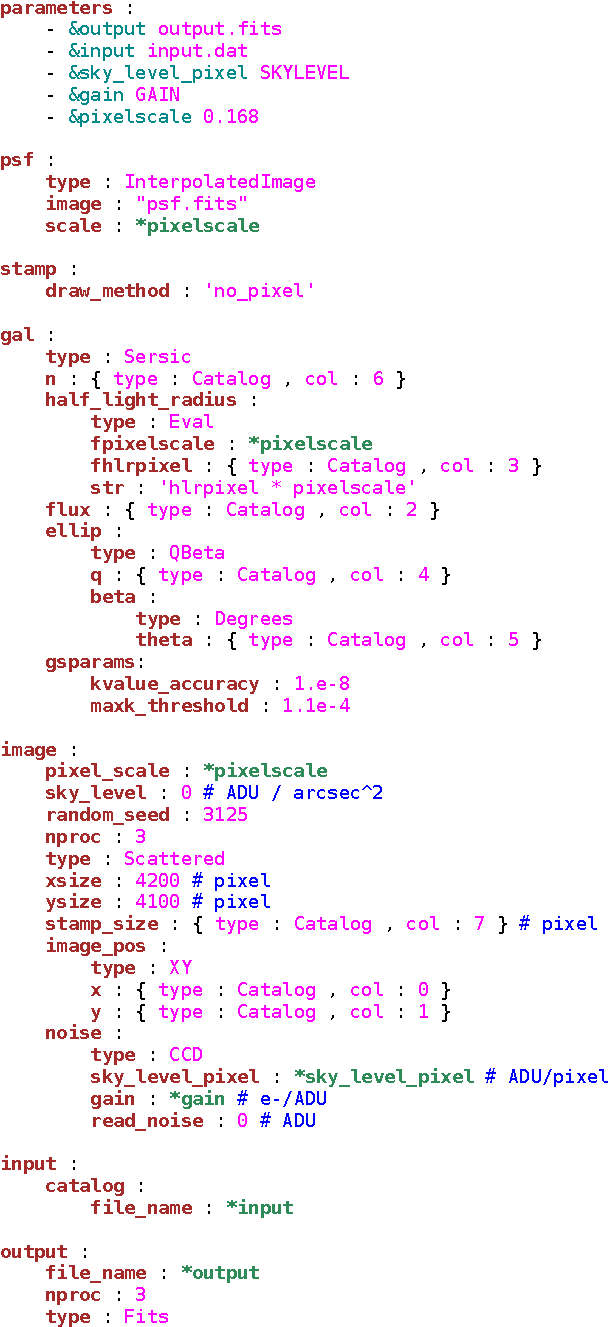
\includegraphics[width=\columnwidth]{{{fig/yamlconfig}}}
    \caption{An example \texttt{YAML} configuration file used as an input to \textsc{GalSim}. This configuration file produces a simulated \texttt{output.fits} file based on the \texttt{input.dat} input catalogue. PSF generation is outlined in Section \ref{sec:psf}, whilst estimates of the original sky level pedestal (\texttt{SKYLEVEL}) and averaged detector equivalent gain (\texttt{GAIN}) are detailed in Section \ref{sec:gainskylevel}. See the text for further information.}
    \label{fig:yamlconfig}
\end{figure}

\section{Postage Stamp Sizes}
\label{sec:postagestampsizes}

We use \SExtractor to fit a single \Sersic function to each detected source as given by a prior run of either \SExtractor, \Gnuastro, or the \LSSTPs. As an output, \SExtractor provides a catalogue containing \Sersic component fitting information, and (optionally) an associated check image containing all successfully fitted \Sersic models in 2D space. Initially, we used the \SExtractor check images as the basis for our modelled masks (see Section \ref{sec:modelledmasking}), however, on closer inspection it became clear that these images were inappropriate for our purposes. 

Figure \ref{fig:modmaskcomp_sex} shows a comparison of \SExtractor model imaging (left panels) to \GalSim model imaging (right panels) using an initial \SExtractor run as the basis for determining which sources should be modelled. The top two panels show these 2D data using a standard arctan stretch, similar to figures found elsewhere in this paper. The bottom two panels show these same data using a narrower stretch, designed to highlight some of the fainter features. As is clear in the lower-left panel, \SExtractor model imaging contains significant artefacts around the edges of \Sersic model sources. The default and immutable \SExtractor postage stamp size is too small, resulting in a visible hard boundary at the edges of most sources. The extent of profile truncation becomes more severe as the source becomes more extended. In addition, notable edge boundary flux-wrapping artefacts are introduced for the brightest of sources, adding a peak of flux to regions where no sources were previously placed. Switching to \GalSim allows us to control the postage stamp box size used for each simulated source, resulting in a smoother and more accurate 2D modelled plane (see lower-right panel in both figures). We opt to define postage stamp boxes for each source such that a source aligned parallel to the $x$-axis would reach a surface brightness limit of $\mu_r=35\,\mathrm{mag}/\mathrm{arcsec}^{-2}$ at the boundary of the postage stamp. This limit was chosen to be sufficiently faint to facilitate exploration of the background sky, yet not too deep to become overly computationally expensive. A minimum postage stamp size of $11\times11$ pixels is enforced at all times.

\begin{figure*}
    \centering
    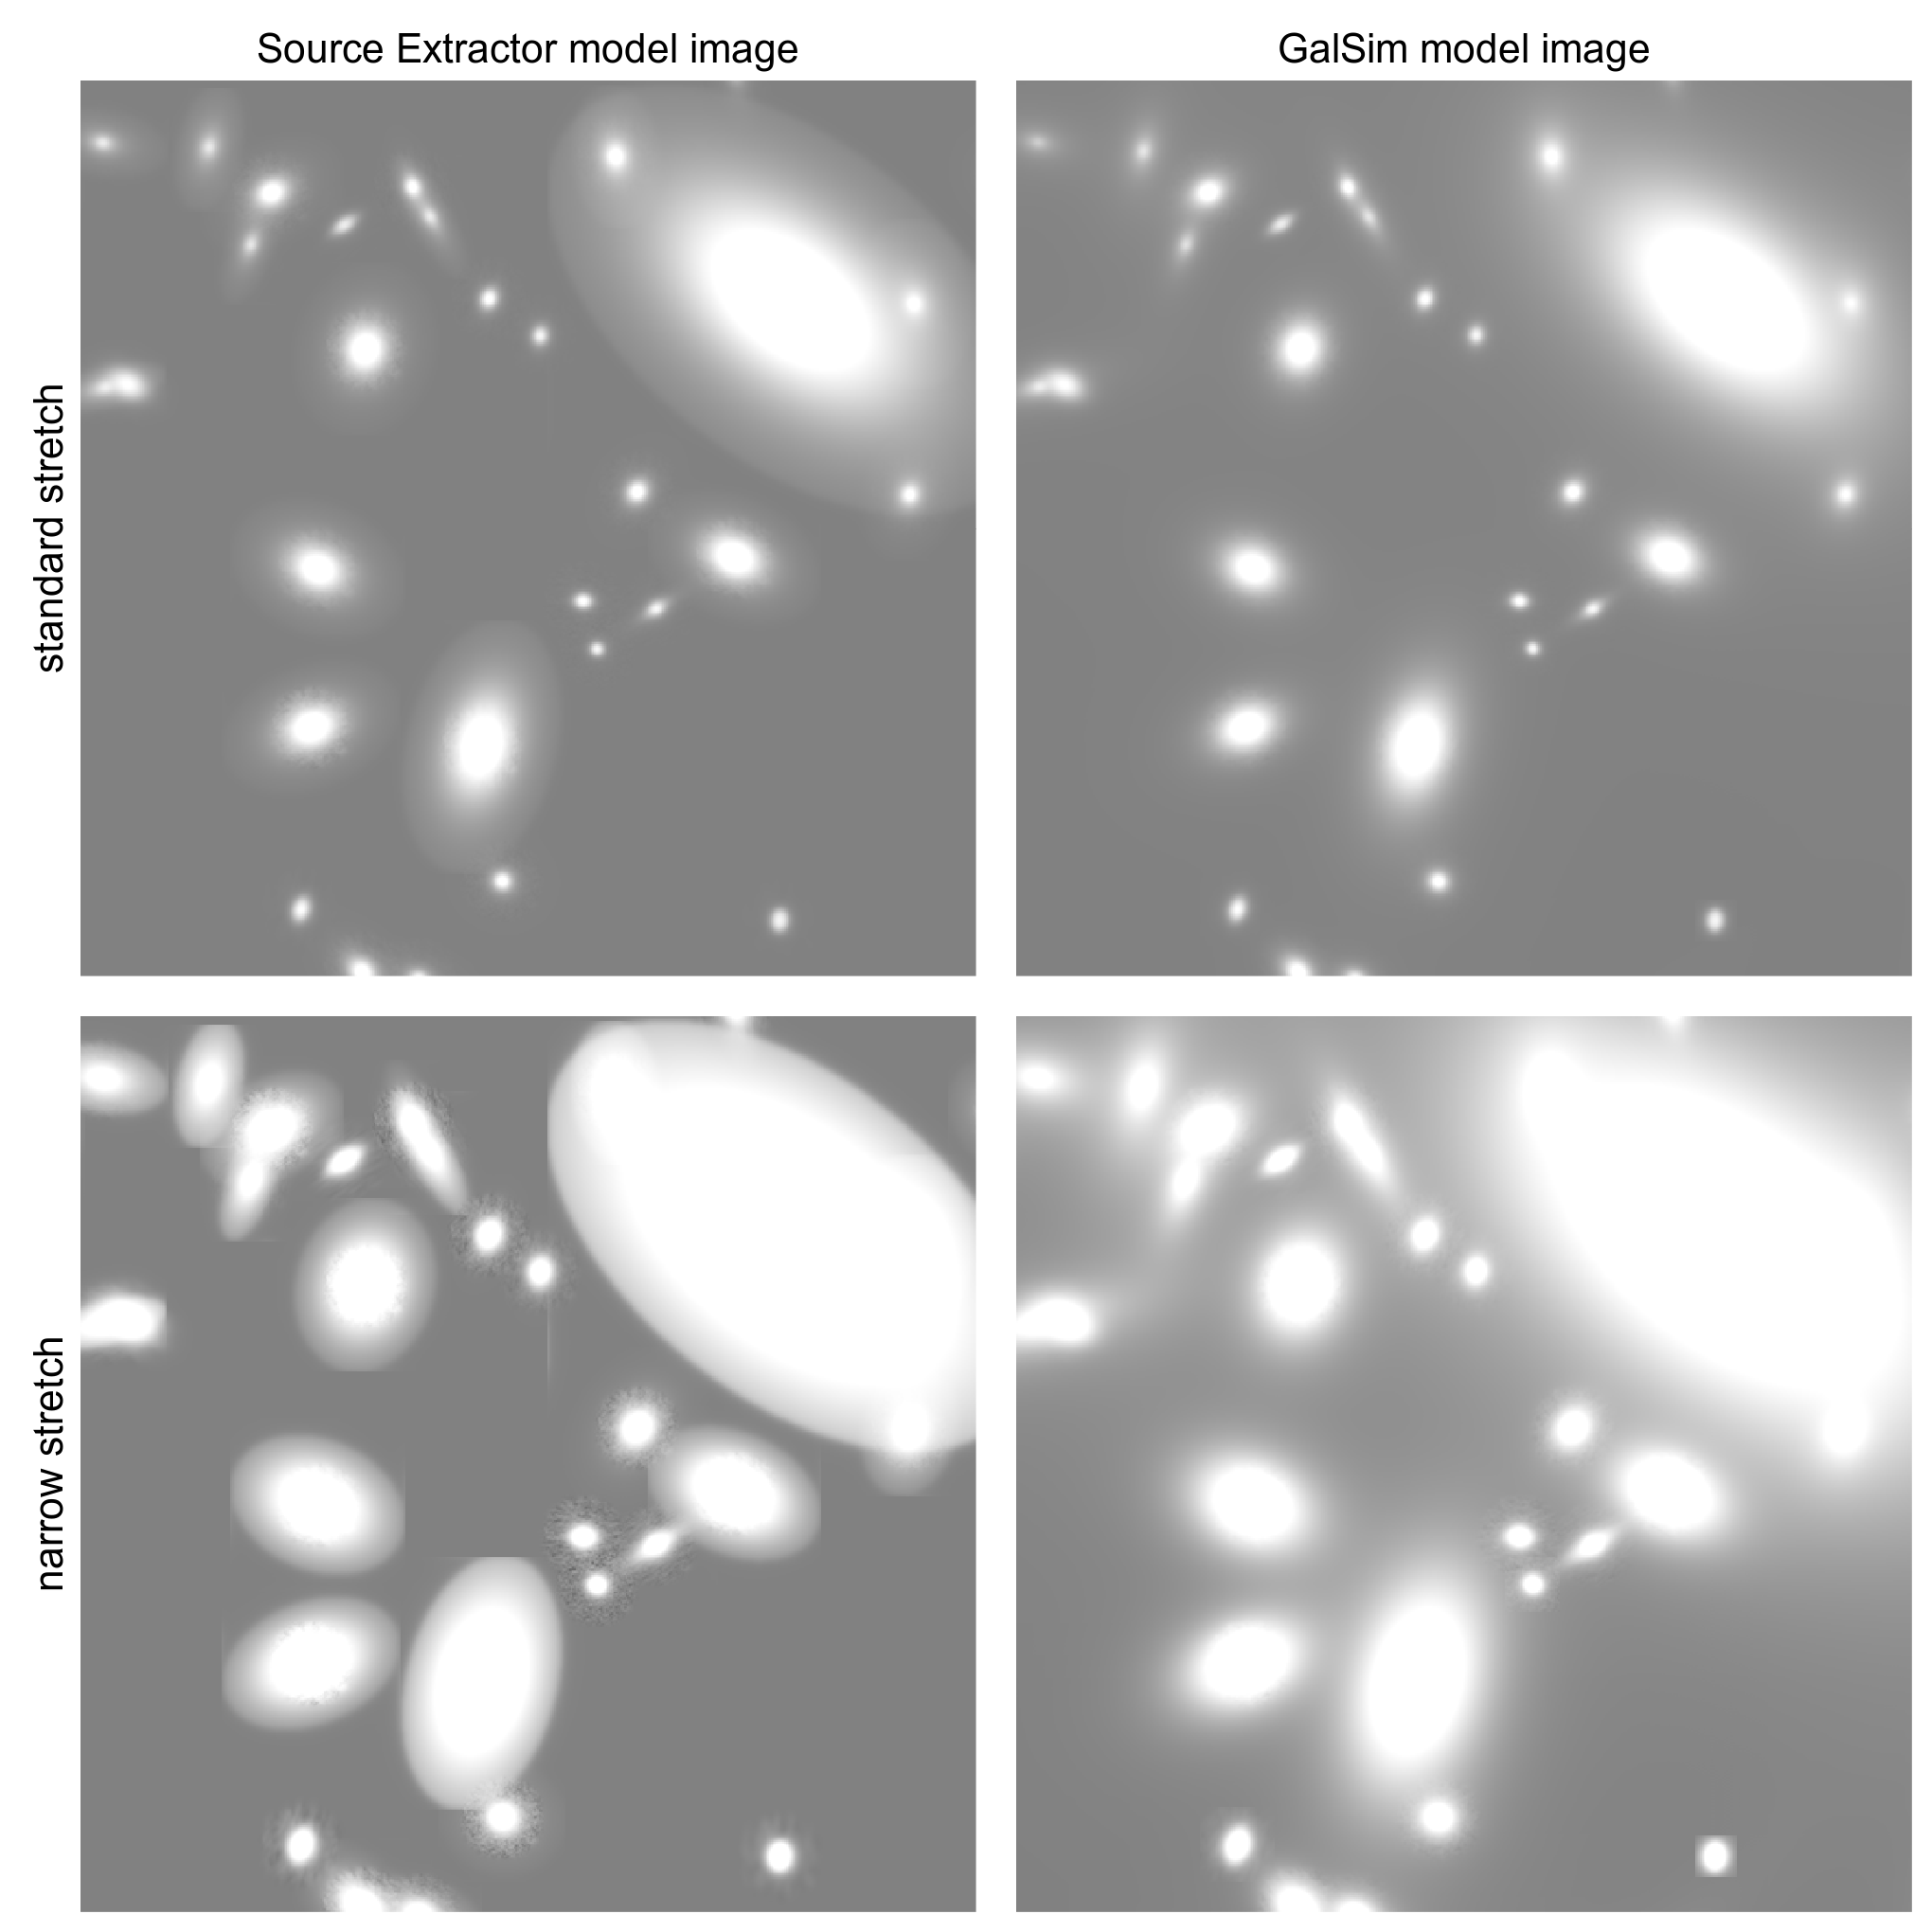
\includegraphics[width=0.9\textwidth]{{{fig/modmaskcomp_sex}}}
    \caption{A comparison of initial \Sersic model imaging produced by \SExtractor (left panels) to our final utilised refined \GalSim \Sersic modelled imaging (right panels). Model \Sersic parameters are derived from \SExtractor. The upper two panels show model imaging using a standard arctan $z$-scale stretch, similar to that found elsewhere in this paper. The lower two panels are arctan scaled over a narrower $z$-scale stretch, highlighting LSB flux around the outskirts of sources. Whilst \SExtractor seemingly produces robust \Sersic catalogue data, it does not allow the user to control the postage stamp size out to which \Sersic models are propagated in an accompanying check image. As a result, various modelled source edge effects are visible (see left panels) in output \SExtractor check imaging owing to the fact that the default \SExtractor postage stamp size is too small for the purposes of this study. We use \GalSim to define bespoke postage stamps for each simulated source (see right panels), minimising this effect.}
    \label{fig:modmaskcomp_sex}
\end{figure*}

% \begin{figure*}
%     \centering
%     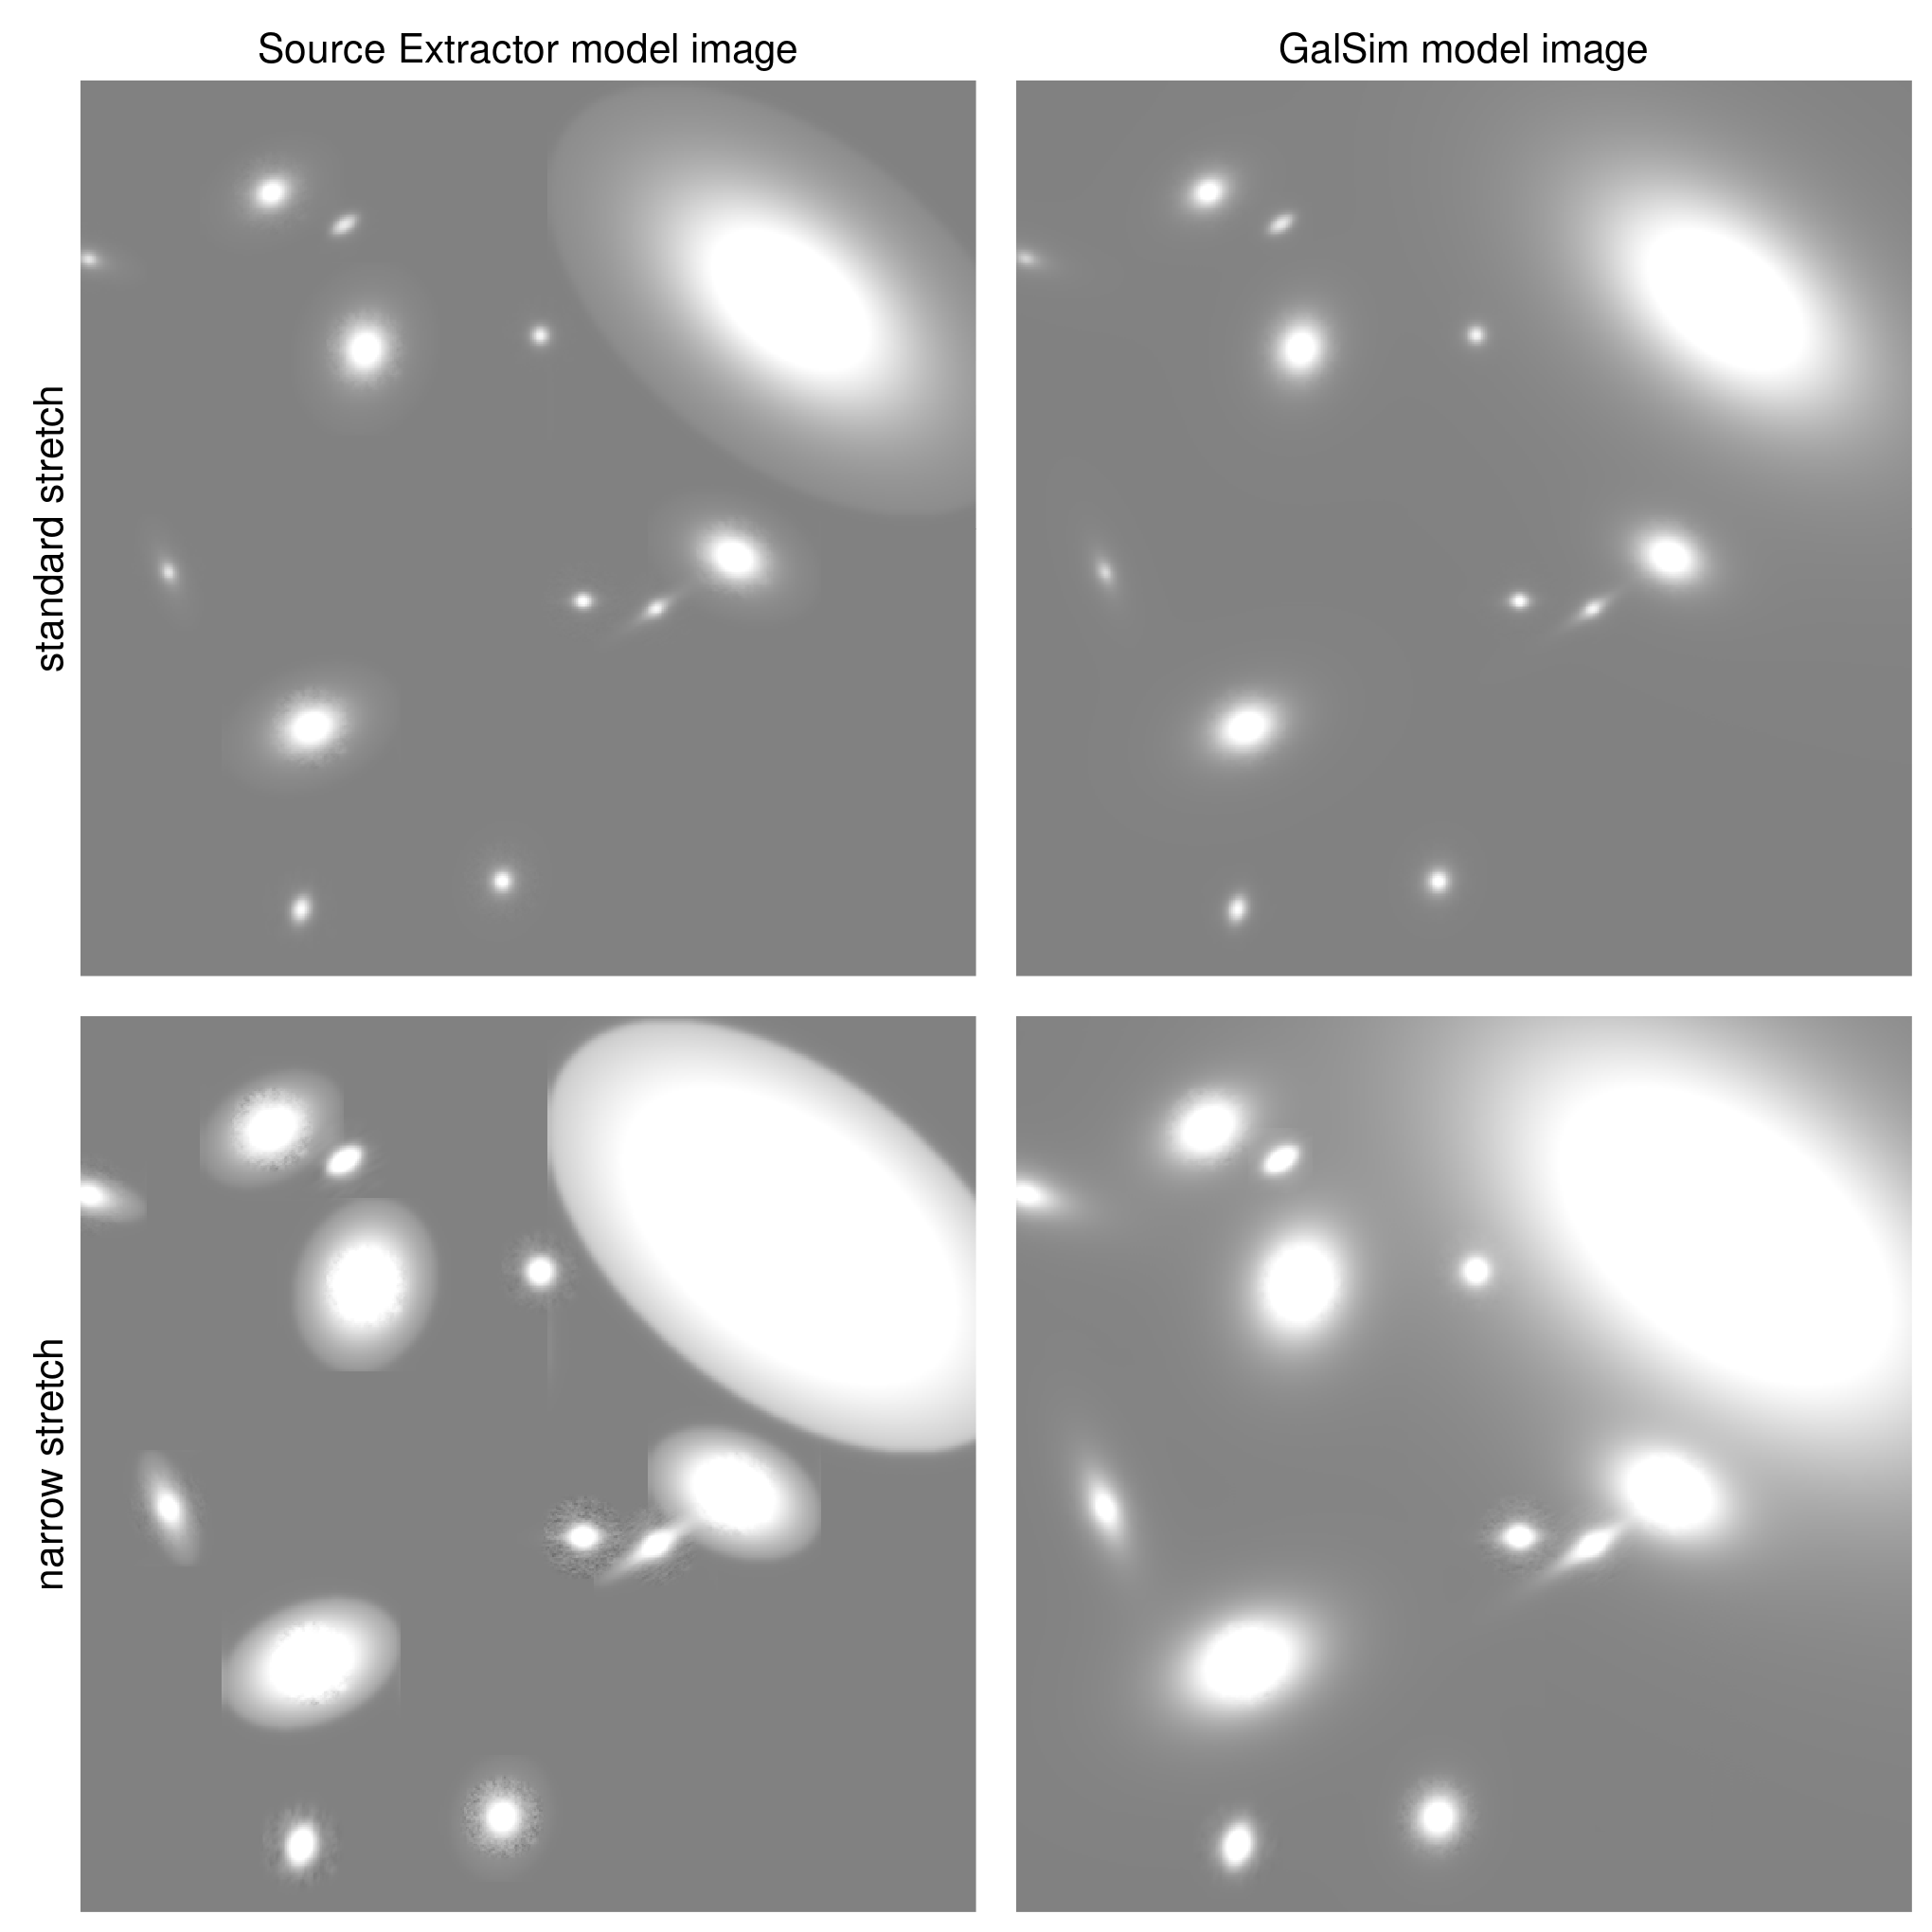
\includegraphics[width=0.9\textwidth]{{{fig/modmaskcomp_gnuastro}}}
%     \caption{A comparison of initial \Sersic model imaging produced by \SExtractor (left panels) to our final utilised refined \GalSim \Sersic modelled imaging (right panels). Model \Sersic parameters are derived from \Gnuastro. The upper two panels show model imaging using a standard logarithmic $z$-scale stretch, similar to that found elsewhere in this paper. The lower two panels are $\arcsinh$ scaled over a narrower $z$-scale stretch, highlighting LSB flux around the outskirts of sources. Whilst \SExtractor seemingly produces robust \Sersic catalogue data, it does not allow the user to control the postage stamp size out to which \Sersic models are propagated in an accompanying check image. As a result, various modelled source edge effects are visible (see left panels) in output \SExtractor check imaging owing to the fact that the default \SExtractor postage stamp size is too small for the purposes of this study. We use \GalSim to define bespoke postage stamps for each simulated source (see right panels), minimising this effect.}
%     \label{fig:modmaskcomp_gnuastro}
% \end{figure*}

%%%%%%%%%%%%%%%%%%%%%%%%%%%%%%%%%%%%%%%%%%%%%%%%%%

% finish up
\label{lastpage}
\end{document}
